% !TeX document-id = {a20f43b2-ab4e-4871-aad0-cb417dac4610}
% !TEX TS-program = xelatex
% Commands for running this example:
% 	 xelatex main
% 	 bibtex8 -W -c cp1256fa main
%      xindy -L persian -C utf8 -M texindy main
% 	 xelatex main
% 	 xelatex main
% End of Commands


\documentclass[oneside,openany,msc]{IUST-Thesis}
\usepackage{xcolor}
\usepackage[many]{tcolorbox}    	% for COLORED BOXES (tikz and xcolor included)
\usepackage{mathspec} 			    % for FONTS
\usepackage{setspace}               % for LINE SPACING
\usepackage{multicol}               % for MULTICOLUMNS
\usepackage{multirow}
%\usepackage{graphicx}
%\usepackage{arydshln}
%\usepackage{bbding}
\usepackage{tablefootnote}

% در این فایل، دستورها و تنظیمات مورد نیاز، آورده شده است.
%-------------------------------------------------------------------------------------------------------------------

% در ورژن جدید زی‌پرشین برای تایپ متن‌های ریاضی، این سه بسته، حتماً باید فراخوانی شود
\usepackage{tabularx,ragged2e}
\newcolumntype{B}{>{\Centering}X}
\newcolumntype{S}{>{\Centering\hsize=.4\hsize}X}
\newcolumntype{M}{>{\Centering\hsize=.6\hsize}X}

\usepackage{amsthm,amssymb,amsmath}
% بسته‌ای برای تنطیم حاشیه‌های بالا، پایین، چپ و راست صفحه
\usepackage[top=40mm, bottom=40mm, left=25mm, right=35mm]{geometry}
% بسته‌‌ای برای ظاهر شدن شکل‌ها و تصاویر متن
\usepackage{graphicx}
% بسته‌ای برای رسم کادر
\usepackage{framed} 
% بسته‌‌ای برای چاپ شدن خودکار تعداد صفحات در صفحه «معرفی پایان‌نامه»
\usepackage{lastpage}
% بسته‌ و دستوراتی برای ایجاد لینک‌های رنگی با امکان جهش
\usepackage[pagebackref=false,colorlinks,linkcolor=blue,citecolor=blue]{hyperref}
% چنانچه قصد پرینت گرفتن نوشته خود را دارید، خط بالا را غیرفعال و  از دستور زیر استفاده کنید چون در صورت استفاده از دستور زیر‌‌، 
% لینک‌ها به رنگ سیاه ظاهر خواهند شد که برای پرینت گرفتن، مناسب‌تر است
%\usepackage[pagebackref=false]{hyperref}
% بسته‌ لازم برای تنظیم سربرگ‌ها
\usepackage{fancyhdr}
%
\usepackage{setspace}
\usepackage{algorithm}
\usepackage{algorithmic}
\usepackage{subfigure}
\usepackage[subfigure]{tocloft}

% بسته‌ای برای ظاهر شدن «مراجع» و «نمایه» در فهرست مطالب
\usepackage[nottoc]{tocbibind}
\usepackage[numbers]{natbib}
% دستورات مربوط به ایجاد نمایه
\usepackage{makeidx}
\usepackage{graphicx} 
\makeindex
%%%%%%%%%%%%%%%%%%%%%%%%%%
% فراخوانی بسته زی‌پرشین و تعریف قلم فارسی و انگلیسی
\usepackage[extrafootnotefeatures]{xepersian}
\settextfont[Scale=1]{XB Niloofar.ttf}
\setlatintextfont[Scale=0.9]{Times New Roman}

%%%%%%%%%%%%%%%%%%%%%%%%%%
% چنانچه می‌خواهید اعداد در فرمول‌ها، انگلیسی باشد، خط زیر را غیرفعال کنید
%\setdigitfont[Scale=1]{XB Zar.ttf}%{Persian Modern}
%%%%%%%%%%%%%%%%%%%%%%%%%%
% تعریف قلم‌های فارسی و انگلیسی اضافی برای استفاده در بعضی از قسمت‌های متن
%\defpersianfont\titlefont[Scale=1]{XB Niloofar.ttf}
% \defpersianfont\iranic[Scale=1.1]{XB Zar Oblique}%Italic}%
% \defpersianfont\nastaliq[Scale=1.2]{IranNastaliq}

\setcounter{tocdepth}{3}
\setcounter{secnumdepth}{3}

%%%%%%%%%%%%%%%%%%%%%%%%%%
% دستوری برای حذف کلمه «چکیده»
\renewcommand{\abstractname}{}
% دستوری برای حذف کلمه «abstract»
%\renewcommand{\latinabstract}{}
% دستوری برای تغییر نام کلمه «اثبات» به «برهان»
\renewcommand\proofname{\textbf{برهان}}
% دستوری برای تغییر نام کلمه «کتاب‌نامه» به «مراجع»
\renewcommand{\bibname}{مراجع}
% دستوری برای تعریف واژه‌نامه انگلیسی به فارسی
\newcommand\persiangloss[2]{#1\dotfill\lr{#2}\\}
% دستوری برای تعریف واژه‌نامه فارسی به انگلیسی 
\newcommand\englishgloss[2]{#2\dotfill\lr{#1}\\}
% تعریف دستور جدید «\پ» برای خلاصه‌نویسی جهت نوشتن عبارت «پروژه/پایان‌نامه/رساله»
\newcommand{\پ}{پروژه/پایان‌نامه/رساله }

%\newcommand\BackSlash{\char`\\}

%%%%%%%%%%%%%%%%%%%%%%%%%%
\SepMark{-}

% تعریف و نحوه ظاهر شدن عنوان قضیه‌ها، تعریف‌ها، مثال‌ها و ...
\theoremstyle{definition}
\newtheorem{definition}{تعریف}[section]
\theoremstyle{theorem}
\newtheorem{theorem}[definition]{قضیه}
\newtheorem{lemma}[definition]{لم}
\newtheorem{proposition}[definition]{گزاره}
\newtheorem{corollary}[definition]{نتیجه}
\newtheorem{remark}[definition]{ملاحظه}
\theoremstyle{definition}
\newtheorem{example}[definition]{مثال}

%\renewcommand{\theequation}{\thechapter-\arabic{equation}}
%\def\bibname{مراجع}
\numberwithin{algorithm}{chapter}
\def\listalgorithmname{فهرست الگوریتم‌ها}
\def\listfigurename{فهرست شکل‌ها}
\def\listtablename{فهرست ‌جدول‌ها}

%%%%%%%%%%%%%%%%%%%%%%%%%%%%
% دستورهایی برای سفارشی کردن سربرگ صفحات
% \newcommand{\SetHeader}{
% \csname@twosidetrue\endcsname
% \pagestyle{fancy}
% \fancyhf{} 
% \fancyhead[OL,EL]{\thepage}
% \fancyhead[OR]{\small\rightmark}
% \fancyhead[ER]{\small\leftmark}
% \renewcommand{\chaptermark}[1]{%
% \markboth{\thechapter-\ #1}{}}
% }
%%%%%%%%%%%%5
%\def\MATtextbaseline{1.5}
%\renewcommand{\baselinestretch}{\MATtextbaseline}
\doublespacing
%%%%%%%%%%%%%%%%%%%%%%%%%%%%%
% دستوراتی برای اضافه کردن کلمه «فصل» در فهرست مطالب

\newlength\mylenprt
\newlength\mylenchp
\newlength\mylenapp

\renewcommand\cftpartpresnum{\partname~}
\renewcommand\cftchappresnum{\chaptername~}
\renewcommand\cftchapaftersnum{:}

\settowidth\mylenprt{\cftpartfont\cftpartpresnum\cftpartaftersnum}
\settowidth\mylenchp{\cftchapfont\cftchappresnum\cftchapaftersnum}
\settowidth\mylenapp{\cftchapfont\appendixname~\cftchapaftersnum}
\addtolength\mylenprt{\cftpartnumwidth}
\addtolength\mylenchp{\cftchapnumwidth}
\addtolength\mylenapp{\cftchapnumwidth}

\setlength\cftpartnumwidth{\mylenprt}
\setlength\cftchapnumwidth{\mylenchp}	

\makeatletter
{\def\thebibliography#1{\chapter*{\refname\@mkboth
   {\uppercase{\refname}}{\uppercase{\refname}}}\list
   {[\arabic{enumi}]}{\settowidth\labelwidth{[#1]}
   \rightmargin\labelwidth
   \advance\rightmargin\labelsep
   \advance\rightmargin\bibindent
   \itemindent -\bibindent
   \listparindent \itemindent
   \parsep \z@
   \usecounter{enumi}}
   \def\newblock{}
   \sloppy
   \sfcode`\.=1000\relax}}
\makeatother


\begin{document}

\pagenumbering{harfi}
% !TeX root=main.tex

\university{علم و صنعت ایران}

\faculty{دانشکده مهندسی کامپیوتر}

\department{گروه هوش مصنوعی}

\subject{مهندسی کامپیوتر}

\field{هوش مصنوعی و رباتیک}

\title{تشخيص موضع متنی در شبکه‌های اجتماعی}

\firstsupervisor{دکتر سید صالح اعتمادی}

\name{غزاله}

\surname{محمودی}

\studentID{400722156}

\thesisdate{بهمن 1402}

\firstPage
\besmPage
\davaranPage

\vspace{.5cm}

%\renewcommand{\arraystretch}{1.2}
\begin{center}
	\begin{tabular}{| p{8mm} | p{18mm} | p{.17\textwidth} |p{14mm}|p{.2\textwidth}|c|}

		\hline
		ردیف	& سمت & نام و نام خانوادگی & مرتبه \newline دانشگاهی &	دانشگاه یا مؤسسه &	امضـــــــــــــا\\
		\hline
		۱  &	استاد راهنما & دکتر سید \newline  صالح اعتمادی & استادیار & دانشگاه \newline علم و صنعت ایران &  \\
		\hline
				۲  &	استاد \newline مدعو داخلی & دکتر  \newline  حسین رحمانی & استادیار & دانشگاه \newline علم و صنعت ایران &  \\
		
		\hline
				۳ &	 استاد \newline مدعو‌‌خارجی& دکتر  \newline سعیده ممتازی & دانشیار & دانشگاه امیرکبیر &  \\
		\hline

	\end{tabular}
\end{center}


%%%%%%%%%%%%%%%%%%%%%%

%\iffalse
\esalatPage
\mojavezPage
\newpage
\iffalse
\thispagestyle{empty}
\centerline{\Large \titlefont  تقـــدیم }
\begin{center}
	محل قرار گرفتن متن قـدرانی و تقدیم در نــسخه نهایی پایان‌نامه. 
\end{center}
\fi

% -- متن سپاس‌گزاری
\begin{acknowledgementpage}
سپاس خداوندگار حکیم را که با لطف بی کران خود، آدمی را زیور عقل آراست و به ما توفیق حرکت در مسیر کسب علم را ارزانی داشت. در آغاز وظیفه خود می‌دانم از زحمات استاد گران‌قدر و فرزانه جناب آقای دکتر سید صالح اعتمادی که راهنمایی اینجانب را در دوره کارشناسی ارشد عهده‌دار بودند، بی‌نهایت سپاس‌گزار هستم. همچنین از آقای بابک بهکام‌کیا که به عنوان همکار در بخشی از پژوهش حضور داشتند کمال تشکر را دارم. در آخر از خانواده عزیزم به پاس حمایت‌های بی دریغ و عاطفه سرشارشان در طول این مدت کمال تشکر و قدردانی را دارم.
	

	% با استفاده از دستور زیر، امضای شما، به طور خودکار، درج می‌شود.
	\signature 
\end{acknowledgementpage}

%\fi
%%%%%%%%%%%%%%%%%%%%%%

%امروزه شبکە‌های اجتماعی بستری جهت آزادانه بیان کردن و به اشتراک گذاشتن عقاید و نظرات می‌باشد. 
\keywords{تشخیص موضع، پردازش زبان طبیعی، یادگیری عمیق، مدل‌های زبانی بزرگ}
\fa-abstract{
امروزه شبکه‌های اجتماعی بستری جهت بیان آزادانه عقاید و اشتراک گذاشتن نظرات می‌باشد. این موضوع سبب شده است که با تحلیل دادە‌های موجود در شبکه‌های اجتماعی بتوان دید وسیع و جامعی از موضع‌ کاربران متفاوت نسبت به موضوعات مختلف به دست آورد. از جمله این موضوعات می‌توان به مسائل سیاسی، اقتصادی، اجتماعی و فرهنگی اشاره کرد. در پردازش زبان طبیعی، به فرآیند تشخیص خودکار موضع متن نسبت به موضوعی مشخص و معین، تشخیص موضع گفته می‌شود. 
\newline
در مسائل پردازش زبان طبیعی از جمله تشخیص موضع، نحوه پیش‌پردازش داده‌های متنی در عملکرد مدل آموزش دیده تاثیر به سزایی دارد. در این پژوهش هفت سطح مختلف پیش‌پردازش معرفی شده و مورد بررسی قرار می‌گیرد. علاوه بر این، برای یافتن معماری مدل تشخیص موضع، از ایده جستجو معماری عصبی (\lr{NAS}) الهام گرفته شد. در این روش با تقسیم معماری مدل به چهار بخش اصلی و تعریف فضای جستجو برای هر بخش و استفاده از الگوریتم‌ جستجو تطبیقی، معماری نهایی طراحی می‌شود. در نهایت بهترین مدل پیشنهاد شده از کدگذار
\lr{BERTweet}
و رده‌بند 
\lr{CNN}
استفاده می‌کند. 
معماری طراحی شده توانست به
$74.47$
درصد در معیار 
\lr{F1} 
دست یابد و نسبت به مدل پایه
$19.97$
درصد بهبود داشته باشد. همچنین روش ارائه شده رتبه سوم را بین 19 شرکت‌کننده رویداد تشخیص موضع در تغییرات اقلیمی کسب کرد. 
از سوی دیگر با توجه به کمبود داده‌های آموزشی برای موضوعات متفاوت، تشخیص موضع بدون داده آموزشی نیز مورد بررسی قرار گرفت. در این روش که از مدل‌های زبانی بزرگ و مهندسی پرامپت استفاده می‌کند، چهار رویکرد بر اساس انواع مختلف پرامپت معرفی شد. سپس عملکرد پرامپت‌های پیشنهادی با سایر روش‌های تشخیص موضع بدون داده آموزشی مورد مقایسه قرار گرفت. رویکرد معرفی شده توانست به مقدار 
$57.33$
درصد در معیار 
\lr{F1} 
دست یابد و نسبت به رویکرد‌های مشابه
$2.03$
درصد بهبود داشته باشد.}
\abstractPage
\newpage\clearpage



\tableofcontents \newpage
\listoffigures   \newpage
\listoftables    \newpage

\pagestyle{fancy}
% !TeX root=main.tex
\pagenumbering{arabic}
\chapter{مقدمه}
\thispagestyle{empty}
امروزه شبکە‌های اجتماعی یکی از اجزا اصلی تعامل اجتماعی افراد را تشکیل می‌دهد. شبکه‌‌های اجتماعی ابزار قدرت‌مندی برای بیان نظرات و دیدگاە‌های افراد در رابطه با موضوعات متفاوت می‌ باشد. این بستر برای افراد این امکان را فراهم می‌کند که آزادانه نظرات خود را بیان کنند و بازخورد فوری دریافت کنند. همچنین دیدگاه سایر افراد در رابطه با موضوع بیان شده را در این بستر می‌توان مورد بررسی قرار داد.


وابستگی افراد به استفاده از شبکه‌‌های اجتماعی این امکان را فراهم می‌کند تا دادە‌های جمع آوری شده از شبکه‌های اجتماعی را به عنوان منبع مهم برای مطالعه جنبە‌های مختلف موضع‌گیری افراد در زمینە‌های سیاسی و اجتماعی مورد استفاده قرار دهیم.


استخراج خودکار اطلاعات از متون زبان طبیعی از مهم‌ترین زمینە‌های تحقیقاتی می‌باشد. در این راستا می‌توان مسئله تشخیص موضع
\LTRfootnote{\lr{Stance Detection}}
 را تعریف کرد. تشخیص موضع به معنای بیان و تشخیص دیدگاه نویسندە‌ی متن نسبت به یگ گزاره‌ی (موضوع) معین است.

تشخیص موضع در مطالعات تحلیلی برای تشخیص جهت گیری افکار عمومی در رسانە‌های اجتماعی، مانند مسائل سیاسی و اجتماعی، نقش کلیدی ایفا می‌کند. از این رو می‌تواند در شبکە‌های اجتماعی در بستراهداف مختلفی از جمله تصمیمات دولت، تبلیغات، اقناع افکار عمومی مورد استفاده قرار بگیرد. به عبارت دیگر نتایج به دست آمده منجر به دید وسیع‌تری به نظرات عمومی و اخذ تصمیمات بهتر می‌شود.
\section{تعریف مسئله تشخیص موضع}
موضع‌گیری
\LTRfootnote{\lr{Stance}}
به بیان دیدگاه و نظرات افراد راجع به یک گزارە‌ی (موضوع) معین گفته می‌شود
\cite{hardalov-etal-2022-survey}.
تشخیص موضع
\LTRfootnote{\lr{Stance Detection}}
نقشی اساسی در شناخت جهت گیری عمومی در رابطه با مسائل اجتماعی و سیاسی، انتخابات و
موضع تصمیمات دولت ایفا می‌کند
\cite{ALDAYEL2021102597, 10.1145/3209542.3209549}.


مسئله تشخیص موضع در شبکه‌های اجتماعی به این صورت تعریف می‌شود که یک متن نوشته شده
در شبکه اجتماعی (توییت، نظرات و ادعا) و یک موضوع یا هدف مشخص
\LTRfootnote{\lr{Target}}
(شخص، سازمان، جنبش،سیاست) به عنوان ورودی در نظر گرفته می‌شود. هدف تشخیص خودکار موضع متن داده شده نسبت به موضوع مشخص شده است
\cite{ALDAYEL2021102597}.
این یک مسئله به صورت ردە‌بندی است و خروجی یکی از موارد زیر می‌تواند باشد
\cite{li-caragea-2019-multi}.
\begin{enumerate}
	\setlength\itemsep{-0.4em}
	\item موافق
	\LTRfootnote{\lr{Favor/Support}}:
	متن مورد نظر، موضوع تعیین شده را بدون هیچ گونه ابهام تایید می‌کند.
	\item مخالف
	\LTRfootnote{\lr{Against/Oppose}}:
	متن مورد نظر، موضوع تعیین شده را بدون هیچ گونه ابهام رد می‌کند.
	\item بدون نظر
	\LTRfootnote{\lr{None/Neither/Neutral}}:
	متن و موضوع به هم مرتبط نیستند و یا متن به صورت صریح موضوع را رد یا تایید نمی‌کند.
	
\end{enumerate}

\begin{figure}[H]
	\center{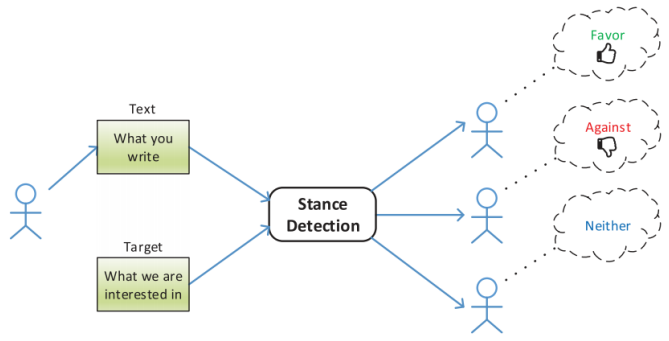
\includegraphics[width=0.6\linewidth]{images/stance_detection.PNG}}
	\caption[تشخیص موضع در شبکه‌های اجتماعی]{تشخیص موضع در شبکه‌های اجتماعی
	\cite{10.1145/3369026}}
\end{figure}

\iffalse
\subsection{کاربردهای تشخیص موضع}
بعد از مطرح شدن تعاریف مختلف مسئله تشخیص موضع، حال به بررسی تعدادی از کاربردهای مطرح شده می‌پردازیم. در مسئله تشخیص موضع، نظر و موضع افراد نسبت به هدف یا موضوع خاص سنجیده می‌شود. با توجه به این تعریف کابردهای زیر مطرح می‌شود.
\begin{enumerate}
	\item 
	 نظرسنجی و بررسی افکار عمومی: مطالعات تشخیص موضع معمولا بر روی محتوا آنلاین انجام می‌شود که موضوع آن مشخص است. از این رو با استفاده از تشخیص موضع خودکار، موافقت یا مخالف عموم افراد جامعه نسبت به موضوع خاصی را می‌توان ارزیابی کرد. این روش می‌تواند جایگزین نظرسنجی‌های سنتی باشد.
	 
	 \item 
	  سیستم‌های توصیە‌گر: در صورتی که موضع افراد نسبت به هدف و موضوعی معین را بدانیم، توصیه کردن محصولات به سادیگی میسر می‌شود.
	 \item 
	 
	 تبلیغات هدفمند: آگاهی از موضع کابران باعث می‌شود تبلیغات به صورت موثر و هدفمند انجام شود.

	 \item
	 
	 تشخیص اخبار جعلی 
	 \cite{popat-etal-2018-declare}
	 و تشخیص شایعه نیز از دیگر کابردهای قابل تعریف به کمک مسئله تشخیص موضع می‌باشند. در این مسائل معمولا از تشخیص موضع ادعا محور استفاده می‌شود.
	 				
\end{enumerate}
\fi
\section{ساختار پایان‌نامه}
این پایان‌نامه در هفت فصل تنظیم شده است. فصل اول مقدمه‌ای از حوزه تحقیقات را شرح می‌دهد. در فصل دوم تعریف مسئله تشخیص موضع به صورت دقیق بیان می‌شود. همچنین جایگاه تشخیص موضع در مقایسه با سایر مسائل مشابه به طور دقیق مشخص می‌شود. فصل سوم به توضیح تعاریف و مفاهیم ابتدایی مورد نیاز برای فهم تشخیص موضع و روش‌های حل مسئله می‌پردازد.
فصل چهارم شامل مروری بر کارهای مرتبط به تشخیص موضع می‌باشد. در فصل پنجم رویکرد حل تشخیص موضع با نظارت شرح داده شده و بررسی می‌شود. فصل ششم نیز شامل معرفی رویکرد پیشنهادی برای تشخیص موضع بدون داده آموزشی می‌باشد. در نهایت در فصل هفتم (فصل آخر) جمع‌بندی از روش‌های حل مسئله انجام شده و پیشنهادهایی برای کارهای آینده ارائه می‌شود.






% !TeX root=main.tex
\pagenumbering{arabic}
\chapter{تعریف مسئله}
\thispagestyle{empty}

تشخیص موضع در مطالعات تحلیلی برای تشخیص جهت گیری افکار عمومی در رسانه‌های اجتماعی، مانند مسائل سیاسی و اجتماعی، نقش کلیدی ایفا می‌کند. از این رو می‌تواند در شبکە‌های اجتماعی در بستر اهداف مختلفی از جمله تصمیمات دولت، تبلیغات، اقناع افکار عمومی مورد استفاده قرار بگیرد. به عبارتی دیگر نتایج به دست آمده منجر به دید وسیع تری به نظرات عمومی و اخذ تصمیمات بهتر می‌شود.


\section{سطوح مسئله تشخیص موضع}\label{sec:stance-detection-level}
قبل از بررسی گونە‌های مختلف تشخیص موضع، شناخت دقیق سطوح مختلف تشخیص موضع از اهمیت
بالایی برخوردار است. مسئله تشخیص موضع معمولا در دو سطح بررسی می‌شود. در ادامه توضیحات
مختصری از این دو سطح را بیان می‌شود.
\begin{enumerate}
	\item 
	 سطح بیانیه
	 \LTRfootnote{\lr{The Statement Level}}
	\newline
در این سطح هدف این است موضع یک متن نوشته شده نسبت به موضوع از قبل مشخص شده،
تعیین گردد. این سطح معمول‌ترین روش به کارگرفته شده در تشخیص موضع است. به صورتی که
ویژگی‌‌های متن نوشته شده استخراج می‌شود و تشخیص موضع صرفا بر اساس متن انجام می‌شود. این مفهوم معمولا به صورت ردە‌بندی با سه کلاس (موافق، مخالف، بدون نظر) تعریف می‌شود.  بدون نظر یعنی متن نوشته شده نسبت به موضوع بی ربط است. حالت دیگر این است که موضوع در
آن بررسی شده ولی موضع مشخصی در رابطه با آن (موافق یا مخالف) ندارد.
	\item  سطح کاربر
	\LTRfootnote{\lr{The User Level}}
	
در این سطح هدف پیشبینی موضع کاربر نسبت به یک موضوع می‌باشد. متغیرهای مختلفی که
یک کاربر از خود در شبکه‌‌های اجتماعی به جای می‌گذارد، در بررسی‌‌ها مورد استفاده قرار می‌گیرد.
پست‌های کاربر، پست‌هایی که پسندیده و یا مجدد به اشتراک گذاشته، از جمله اطلاعاتی‌ است که در این فرآیند مورد استفاده قرار می‌گیرد. در این سطح معمولا ردە بندی با دو کلاس (موافق و مخالف) تعریف می‌شود. چرا که این فرض در نظر گرفته شده که حتی اگر بعضی از پست‌های کاربر در رابطه با موضوع معین بدون موضع باشد، اما به هر حال کاربر یک موضع مشخصی نسبت به آن موضوع دارد.

\end{enumerate}

آشنایی با سطوح مختلف تشخیص موضع و تفاوت آن‌ها بسیار با اهمیت است. پست‌های مختلف یک کاربر نسبت به یک موضوع می‌تواند موضع‌های مختلفی داشته باشد. ولی‌ زمانی که در سطح کاربر مسئله تشخیص موضع را تعریف می‌کنیم، موضع کلی کاربر نسبت به موضوع مطرح می‌شود.

\section{تقسیم بندی تشخیص موضع بر اساس موضوع}
در تشخیص موضع همان‌طور که در گذشته بیان کردیم، نیاز به مشخص بودن یک موضوع (هدف) برای تشخیص موضع در رابطه با آن وجود دارد.

\subsection[تشخیص موضع برای یک موضوع خاص]{تشخیص موضع برای یک موضوع خاص\LTRfootnote{\lr{Target-specific Stance Detection}}
}
رایج ترین نوع تشخیص موضع در شبکه‌های اجتماعی، تشخیص موضع برای یک موضوع خاص است. در
این نوع تشخیص موضع متن یا کاربر، ورودی اصلی برای پیش‌بینی موضع نسبت به یک هدف مشخص است. بنابراین برای هر هدف یک مدل ردە‌بندی جداگانه آموزش داده می‌شود.

\subsection[تشخیص موضع برای موضوعات چندگانه مرتبط]{تشخیص موضع برای موضوعات چندگانه مرتبط\LTRfootnote{\lr{Multi-Related-Target Stance Detection}}}
در این روش، تشخیص موضع نسبت به چندین هدف مرتبط انجام می‌شود. این هدف‌ها می‌توانند یک موضوع کلی، رویداد خاص و یا اشخاص مختلف باشند. دادە‌های یک هدف می‌تواند دانشی برای هدف‌های دیگر داشته باشد. به عنوان مثال فردی که موافقت خود را با یکی از نامزدهای انتخابات ریاست جمهوری اعلام می‌کند، به صورت متوالی مخالف خود را با نامزد حزب (گروه) مقابل نیز اعلام کرده است.

لازم به ذکر است نوع دیگری از تشخیص موضع با عنوان تشخیص موضع برای موضوع متقابل
\LTRfootnote{\lr{Cross-Target Stance Detection}}
نیز تعریف شده است. در این روش آموزش مدل بر روی یک موضوع مشخص انجام می‌شود. در مرحله ارزیابی دادە‌های موضوع متفاوت اما مرتبط با موضوع زمان آموزش مورد استفاده قرار می‌گیرد. در شرایطی که مجموعه داده کافی برای آموزش مدل با بهترین عملکرد در دسترس نباشد، یکی از ایدە‌های قابل استفاده این مورد می‌باشد. به عنوان مثال در پژوهش 
\cite{xu-etal-2018-cross}
آموزش مدل بر روی دادە‌ها با برچسب هیلاری کلینتون انجام می‌شود. در زمان ارزیابی از دادە‌ها با برچسب دونالد ترامپ استفاده می‌شود. در واقع همچون حالت قبل مدل
به نوعی آموزش می‌بیند که بتواند برای دو موضوع متفاوت ولی مرتبط عملیات تشخیص موضع را انجام دهد.

\subsection[تشخیص موضع ادعا محور]{تشخیص موضع ادعا محور
\LTRfootnote{\lr{Claim-Based Stance Detection}}}
در این حالت هدف تشخیص موضع، یک هدف مشخص (صریح) مثل شخص، رویداد نیست. در واقع هدف
در اینجا می‌تواند ادعای عنوان خبر یا شایعه باشد. در ادامه برای آشنایی بیشتر با مسائل مرتبط و فهم جایگاه مسئله اصلی، توضیح دقیق‌تر انواع آن و برچسب‌های موجود در هر مورد را بررسی می‌کنیم.
\begin{enumerate}
	\item  
	تشخیص موضع در اخبار جعلی
	\LTRfootnote{\lr{Fake News Stance Detection}}
	\newline
	در این حالت ورودی تیتر خبر
	\LTRfootnote{\lr{News Headline}}
	به همراه یک متن خبری کامل
	\LTRfootnote{\lr{News Body}}
	می‌باشد (تیتر خبر و متن خبر ممکن است برای دو خبر کاملا متفاوت باشند). در نهایت هدف این است موضع متن خبری نسبت به ادعا مطرح شده در تیتر خبر مورد بررسی قرار بگیرد. این مسئله به صورت ردە‌بندی با‌ چهار کلاس (تایید‍~
			\LTRfootnote{\lr{Agrees}}، رد
			\LTRfootnote{\lr{Disagrees}}
	، بحث شده (موضوع مرتبط بدون نظر قطعی)
			\LTRfootnote{\lr{Discusses}}
	، نامرتبط
			\LTRfootnote{\lr{Unrelated}}
	) تعریف می‌‌شود. این مسئله برای حل تشخیص اخبار جعلی مطرح می‌شود.
	\item 
	تشخیص شایعه
	\LTRfootnote{\lr{Rumer Stance Detection}}
	\newline
	در این حالت ورودی شایعه به همراه یک قطعه متن است. هدف این است موضع نویسنده متن نسبت به صحت شایعه مطرح شده سنجیده شود. این مسئله به صورت ردە‌بندی تعریف می‌شود. در بعضی تعاریف ردە‌بندی با چهار کلاس شامل (تایید
		\LTRfootnote{\lr{Supporting}}
	، رد
		\LTRfootnote{\lr{Denying}}
	، پرس و جو
			\LTRfootnote{\lr{Querying}}
	 و اظهارنظر
	 		\LTRfootnote{\lr{Commenting}}
	 ) تعریف می‌شود. در برخی دیگر از تعاریف ردە‌بندی با دو کلاس (تایید
		\LTRfootnote{\lr{Supporting}}
	 و رد
	 	\LTRfootnote{\lr{Denying}}
	 ) تعریف می‌شود.
\end{enumerate}
\subsection{تفاوت تشخیص موضع و تحلیل احساسات}
مسئله تحلیل احساسات
	\LTRfootnote{\lr{Sentiment Analysis}}
	به عنوان مسئله پردازش احساسی متون در نظر گرفته می‌شود که می‌تواند بدون
	داشتن یک هدف مشخص استنباط شود. در این مسئله مشخص می‌شود یک متن نوشته شده بر اساس محتوای زبان، احساس مثبت
		\LTRfootnote{\lr{Positive}}،
		منفی
		\LTRfootnote{\lr{Negative}}
			یا خنثی
		\LTRfootnote{\lr{Neutral Sentiment}}
				دارد.  در حالی که در تشخیص موضع موافق یا مخالف بودن
			نویسنده متن با موضوع مشخص شده، مد نظر است. شکل
			\ref{sem-eval-label}
توزیع برچسب‌های تحلیل احساسات نسبت به تشخیص موضع در مجموعه داده
			 \lr{SEM-Eval2016}
			\cite{Sobhani2016DetectingSI}
را نشان می‌دهد. برچسب‌های تحلیل احساسات و تشخیص موضع همیشه یکسان نیست. به عنوان مثال تمام دادگانی که در تحلیل احساسات برچسب مثبت دارند، در تشخیص موضع برچسب موافق نگرفتە‌اند. حدود ۳۰ درصد موافق و حدود ۳۳ درصد مخالف و مابقی نیز برچسب خنثی دارند.
\begin{figure}[H]
	\vspace{-0.5cm}
	\center{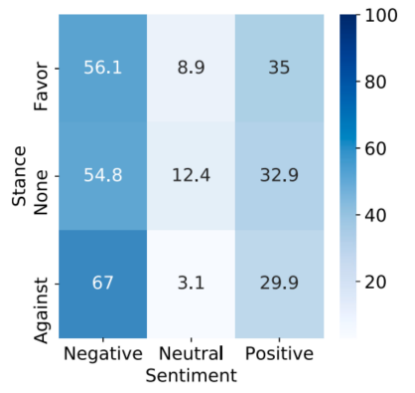
\includegraphics[width=0.4\linewidth]{images/sem-eval-label.PNG}}
	\caption[توزیع برچسب‌های تحلیل احساسات نسبت به برچسب‌های تشخیص موضع]{توزیع برچسب‌های تحلیل احساسات نسبت به برچسب‌های تشخیص موضع در مجموعه دادگان
	\lr{SEM-Eval2016} \cite{ALDAYEL2021102597}\label{sem-eval-label}}
	
\end{figure}	



\begin{table}[h!]
\caption[نمونه‌ای از مجموعه داده
	\lr{SemEval}]{نمونه‌ای از مجموعه داده
\lr{SemEval}\cite{ALDAYEL2021102597}\label{example}}
	\centering
	\begin{tabular}{c  c c c}

		متن توییت & موضوع & تشخیص موضع & تحلیل احساسات
		\\
		\hline
	
				\begin{tabular}{@{}c@{}}
						\lr{I am sad that Hillary lost} \\ 
						\lr{this presidential race.}\\
			    \end{tabular}
				 & \lr{Hillary Clinton} & موافق & منفی
		\\
		\hline
	\end{tabular}

\end{table}
به عنوان مثال و برای درک بهتر جمله و هدف حدول
\ref{example}
 را در نظر بگیرید 
\cite{mohammad-etal-2016-semeval}.
نویسنده متن، با متن نوشته شده نشان می‌دهد با کلینتون موافق است. در حالی‌ که از نظر احساسات، متن احساس منفی منتقل می‌کند. بنابراین می‌توان نتیجه گرفت دو مسئله تحلیل احساسات و تشخیص موضع به هم مرتبط هستند اما یکسان
نیستند 
\cite{Sobhani2016DetectingSI}.

پس به طور خلاصه دو تفاوت عمده مسئله تشخیص موضع و تحلیل احساسات شامل موارد زیر می‌شود. (۱)در تشخیص موضع، موضوع که نسبت به آن بررسی‌ها انجام می‌شود به طور کامل مشخص است. (۲)مانند مثال بالا برچسب‌های نهایی این دو مسئله می‌توانند کاملا با هم متفاوت باشد. بنابراین تفاوت این دو	مسئله کاملا مشهود است.

تحلیل احساسات جنبه گرا
	\LTRfootnote{\lr{Aspect-Oriented Sentiment Analysis}}
شبیە ترین مسئله موجود به تشخیص موضع می‌باشد. در این نوع از تحلیل احساسات موضوع معمولا شامل محصولات الکترونیکی(لپتاپ)، رستوران و هتل می‌باشد. جنبە‌های مورد بررسی نیز شامل قیمت، کیفیت، طرح می‌باشد. تفاوت تحلیل احساسات جنبه‌گرا با تشخیص موضع در این است که در تحلیل احساسات موضوعی که مورد بررسی قرار می‌گیرد در متن به صورت دقیق ذکر شده است. اما در تشخیص موضع لزوما این طور نیست. همچنین موضوع مورد بررسی در تشخیص موضع می‌تواند یک رویداد باشد ولی در تحلیل احساسات جنبە‌گرا این طور نیست.

\begin{figure}[H]
	\center{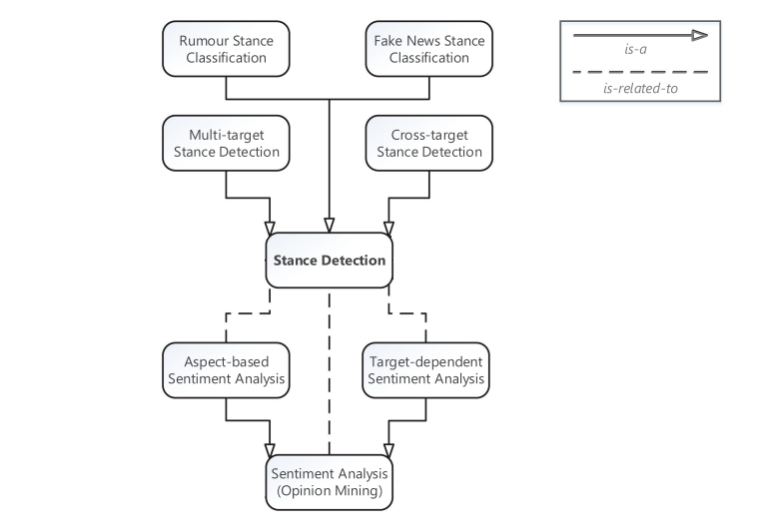
\includegraphics[width=0.8\linewidth]{images/stance_related_research.PNG}}
	\caption[موضوعات تحقیقاتی مرتبط با تشخیص موضع]{
		موضوعات تحقیقاتی مرتبط با تشخیص موضع
		 \cite{10.1145/3369026}\label{stance_related_research}}
	
\end{figure}

\subsection{کاربردهای تشخیص موضع}
بعد از مطرح شدن تعاریف مختلف مسئله تشخیص موضع، حال به بررسی تعدادی از کاربردهای مطرح شده می‌پردازیم. در مسئله تشخیص موضع، نظر و موضع افراد نسبت به هدف یا موضوع خاص سنجیده می‌شود. با توجه به این تعریف کابردهای زیر مطرح می‌شود.
\begin{enumerate}
	\item 
	 نظرسنجی و بررسی افکار عمومی: مطالعات تشخیص موضع معمولا بر روی محتوا آنلاین انجام می‌شود که موضوع آن مشخص است. از این رو با استفاده از تشخیص موضع خودکار، موافقت یا مخالف عموم افراد جامعه نسبت به موضوع خاصی را می‌توان ارزیابی کرد. این روش می‌تواند جایگزین نظرسنجی‌های سنتی باشد.
	 
	 \item 
	  سیستم‌های توصیە‌گر: در صورتی که موضع افراد نسبت به هدف و موضوعی معین را بدانیم، توصیه کردن محصولات به سادیگی میسر می‌شود.
	 \item 
	 
	 تبلیغات هدفمند: آگاهی از موضع کابران باعث می‌شود تبلیغات به صورت موثر و هدفمند انجام شود.

	 \item
	 
	 تشخیص اخبار جعلی 
	 \cite{popat-etal-2018-declare}
	 و تشخیص شایعه نیز از دیگر کابردهای قابل تعریف به کمک مسئله تشخیص موضع می‌باشند. در این مسائل معمولا از تشخیص موضع ادعا محور استفاده می‌شود.
	 				
\end{enumerate}



% !TeX root=main.tex

\chapter{تعاریف و مفاهیم ابتدایی}
\thispagestyle{empty}

در این فصل، توضیحات مختصری در ارتباط با مفاهیم و تعاریف اولیه ارائه شده است. توضیحات ارائه شده، پیش زمینە‌ای برای فهم بهتر مسئله تشخیص موضع در شبکه‌های اجتماعی می‌باشد.

\section{شبکه‌های اجتماعی}
شبکه‌های اجتماعی
\LTRfootnote{\lr{Social Media}}
یک فناوری مبتنی بر رایانه است که قابلیت به اشتراک گذاری ایدە‌ها، افکار و اطلاعات
را از طریق شبکه‌ها و جوامع مجازی فراهم می‌کند. شبکه‌‌های اجتماعی معمولا توسط مجموعە ای از افراد شکل گرفته است که دیدگاە‌های خود را بیان کرده و در رابطه با آن تبادل نظر می‌کنند.

امروزه، بسیاری از تعاملات اجتماعی افراد در بستر شبکه‌های اجتماعی انجام می‌شود. مردم برای برقراری ارتباطات، اطلاع از اخبار و بررسی دیدگاه افراد دیگر از این رسانە‌ها استفاده می‌کنند
\cite{CAN2021101501}.
در شبکه‌های اجتماعی هر فرد می‌توانند آزادانه دیدگاه خود را مطرح کنند. همچنین از دیدگاه سایر افراد نیز مطلع می‌شود. علاوه بر همه موارد کشف دیدگاه عموم جامعه با رصد شبکه‌های اجتماعی تا حد خوبی امکان پذیر است. استفاده گروه عظیمی از کاربران از شبکه‌های اجتماعی این فرصت ر ا فراهم می‌کند تا جنبە‌های مختلف رفتار انسان از جمله موضع گیری عمومی نسبت به جنبە‌های مختلف اجتماعی و سیاسی، قابل تحلیل
باشد
\cite{ALDAYEL2021102597}.

\section{هوش مصنوعی}
هوش مصنوعی
\LTRfootnote{\lr{Artificial Intelligence}}
به فرآیند هوشمندسازی کامپیوتر برای یادگیری و تفکر گفته می‌شود. در این فرآیند هدف این است کامپیوتر همچون انسان توانایی حل مسئله و تصمیم گیری را یاد بگیرد. این اصطلاح عموما به پروژە‌هایی اطلاق می‌شود که توانایی استدلال، یادگیری از تجربیات گذشته و کشف معنا و الگو را دارند. همچنین با کمک اطلاعاتی که جمع می‌کند مکررا می‌تواند توانایی خود را بهبود دهد.

سیستم‌های توصیه‌گر
\LTRfootnote{\lr{Recommendation System}}،
دستیار هوشمند
\LTRfootnote{\lr{Intelligent Assistants}}،
موتورهای جستجو و تشخیص صدا یا دستخط از جمله کاربردهایی هستند که از دانش هوش مصنوعی استفاده می‌کنند.

\section{پردازش زبان طبیعی}
پردازش زبان طبیعی
\LTRfootnote{\lr{Artificial Intelligence}}
یکی از شاخە‌های هوش مصنوعی می‌باشد. هدف این است که کامپیوتر بتواند زبان
انسان را درک و تفسیر کند. این فرآیند شامل تبدیل گفتار به متن، آموزش مدل برای تصمیم گیری و انجام اقدامات هوشمندانه است. پردازش زبان طبیعی بر روی دادە‌های بدون ساختار کار می‌کند و به عوامل مختلفی از جمله دستور زبان، لحن و احساسات وابسته است
\cite{Chowdhary2020}.

برای درک بهتر زبان انسان توسط کامپیوتر مراحل مختلفی از جمله تحلیل واژگانی
\LTRfootnote{\lr{Lexical Analysis}}،
تحلیل نحوی
\LTRfootnote{\lr{Syntactical Analysis}}
و تحلیل معنایی
\LTRfootnote{\lr{Semantic Analysis}}
به کار گرفته می‌شود. با توجه به پیچیدە بودن فهم زبان انسان، زیر شاخه پردازش زبان طبیعی نیز یکی از پیچیدە ترین زیرشاخە‌های هوش مصنوعی در نظر گرفته می‌شود. ترجمه ماشینی
\LTRfootnote{\lr{Machine Translation}}،
حلاصه‌سازی متون
\LTRfootnote{\lr{Text Summarization}}
و تحلیل احساسات
\LTRfootnote{\lr{Sentiment Analysis}} 
از جمله کاربردهای پردازش زبان طبیعی می‌باشد. همچنین مترجم گوگل
\LTRfootnote{\lr{Google Translate}}
یکی از محبوب‌ترین ابزارهایی می‌باشد که در آن از الگوریتم‌های پردازش زبان طبیعی استفاده شده است.
\section{تعبیه کلمات}
در پردازش زبان طبیعی نمی‌توان متن را به صورت ساده و خام به عنوان ورودی به الگوریتم داد. بنابراین نیاز است کلمات در قالب بردارهای عددی قابل فهم و پردازش توسط کامپیوتر به آن وارد شوند. تعبیه کلمات~
\LTRfootnote{\lr{Machine Learning}}
به فرآیند نگاشت کلمات یا عبارات به بردارهای عددی قابل پردازش توسط کامپیوتر گفته می‌شود. این روش به طور معمول برای مدل‌سازی زبان و آمادە‌سازی متن جهت استفاده از آن در الگوریتم های پردازش زبان طبیعی استفاده می‌شود. رویکردهای مختلفی برای بازنمایی کلمات وجود دارد که در ادامه معروف‌ترین روش‌ها را مورد بررسی قرار خواهیم داد.
\begin{enumerate}
	\item کدگذاری
	\lr{one-hot}
	
	روش کدگذاری
	 \lr{one-hot}
	 سادە‌ترین و ابتدایی‌ترین روش استفاده شده برای تعبیه کلمات است. در این روش
	طول بردار تولید شده برای هر کلمه، برابر با تعداد کلمات یکتا در مجموعه دادگان مورد بررسی می‌باشد. در بردارهای تولید شده توسط این روش، یکی از درایە‌های بردار مقدار یک و بقیه درایە‌ها مقدار صفر می‌گیرند. پیادە‌سازی این روش بسیار آسان است. اما در صورت بزرگ بودن مجموعه داده، طول بردار بازنمایی کلمات بسیار بزرگ خواهد بود. همچنین عیب دیگر این روش این است که مفهومی از کلمات را در خود جای نداده است. به این دلیل که فاصله کلیه کلمات مجموعه دادگان از یکدیگر یکسان است. بنابراین بازنمایی تولید شده، فرقی مابین کلمات مترادف و یا کلمات بی ربط ایجاد نمی‌کند. در صورتی که انتظار ما این است 	فاصله بردار کلمات مترادف از یکدیگر نسبت به کلمات بی ربط به یکدیگر متفاوت باشد.
	\item کدگذاری
	\lr{TF-IDF}
	
	روش
\lr{TF-IDF}\LTRfootnote{\lr{Term Frequenct-Inverse Document Frequency}}
یکی دیگر از روش‌های مورد استفاده است. هدف از این روش، تنظیم کردن و یک دست کردن کلماتی است که بارها در متن تکرار شدە اند. متن می‌تواند شامل یک سند یا مجموعە‌ای از اسناد مختلف باشد. این روش ترکیبی از دو معیار است.
\begin{itemize}
	\item   
	\lr{TF} : 
	که عبارت است از تقسیم تعداد تکرار کلمه بر کل کلمات محتوا.
	\item   
	\lr{IDF}: 
	فراوانی سند معکوس. عبارت است از لگاریتم تقسیم تعداد کل اسناد موجود بر محتواهایی که شامل کلمه مورد نظر می‌شوند.
\end{itemize}
لازم به ذکر است
\lr{TF-IDF}
نمی‌تواند مفهوم کلمه در یک جمله را به خوبی نمایش دهد. در واقع کلمات به
بردارهایی تبدیل می‌شوند ولی توجهی به معنی کلمه در جمله نمی‌شود.

\item کدگذاری
\lr{Word2Vec}

روش
\lr{Word2Vec}\cite{41224}
یکی دیگر از روش‌های مورد استفاده برای تعبیه کلمات است. این روش کل پیکره را به عنوان ورودی می‌گیرد و کلمات را به یک بردار چند بعدی نگاشت می‌کند. بر خلاف روش
\lr{one-hot}
 در این روش بردارهای تولید شده مفاهیمی از کلمه را در خود جای دادە اند. بنابراین کلمات مشابه، بردارهای مشابه دارند. این الگوریتم دو مدل مبتنی بر شبکه عصبی ارائه  می‌دهد که در ادامه هر کدام را بررسی می‌کنیم.
 \begin{itemize}
 	\item \lr{CBOW}:
 	در این روش کلمات اطراف و نزدیک به یک کلمه به عنوان ورودی به شبکه دادە می‌شود و هر کلمه میانی به عنوان کلمه هدف در نظر گرفته می‌شود. وظیفه مدل این است با توجه به کلمات اطراف، بردار مناسب برای کلمه هدف (کلمه میانی) را تولید کند.
 	\item \lr{Skip-Gram}:
 	این روش دقیقا برعکس روش \lr{CBOW} می‌باشد. در این روش شبکه عصبی یک کلمه را به عنوان ورودی می‌گیرد و وظیفه دارد چند کلمه قبل و چند کلمه بعد از کلمه ورودی را پیشبینی کند.
 	
 \end{itemize}
\item کدگذاری
\lr{GloVe}

یکی دیگر از روش‌های تولید بردار تعبیه کلمات
\lr{GloVe}\LTRfootnote{\lr{Global Vector}}\cite{pennington-etal-2014-glove}
می‌باشد. این روش در سال ۲۰۱۴ در تیم پردازش زبان طبیعی استنفورد معرفی شده است. این روش به صورت بدون ناظر با تجمیع ماتریس هم زمانی
کلمه به کلمه سراسری 
\LTRfootnote{\lr{Global word-word co-occurrence matrix}}
 یک پیکره، یک بردار جانمایی برای هر کلمه تولید می‌کند.
 
 \item تولید بازنمایی متن با استفاده از 
 \lr{CNN ,GRU ,LSTM}
 
 با پیشرفت یادگیری عمیق در دهە‌های اخیر، پژوهشگران برای بازنمایی متن و استخراج ویژگی از شبکەهای
  \lr{CNN}\cite{kim-2014-convolutional}، \lr{LSTM} و \lr{GRU}
  نیز استفاده می‌کنند. برای استخراج ویژگی با استفاده از
 \lr{CNN}
  بردارهای کلمات در کنار یکدیگر قرار می‌گیرند. سپس به لایه پیچشی
  \LTRfootnote{\lr{Convolution Layer}}
یک بعدی داده می‌شوند و طی مراحل مختلف فیلترهای مختلفی بر روی آن‌ها اعمال می‌شود. در انتها پس از عبور از لایه
\lr{max-pooling}
ویژگی‌های مورد نظر از متن به دست می‌آید. بدین ترتیب از شبکه
 \lr{CNN}
 در پردازش زبان طبیعی برای استخراج ویژگی از متن استفاده می‌شود. شکل 
 \ref{cnn-embedding}
 فرآیند تولید بازنمایی متن با استفاده از شبکه 
  \lr{CNN} 
 را نشان می‌دهد. برای تولید بازنمایی متن توسط LSTM و GRU کافیست جمله (عبارت) مورد نظر به عنوان ورودی به شبکه داده شود. خروجی آخرین گام زمانی به عنوان بازنمایی جمله (عبارت) ورودی در نظر گرفته می‌شود.
 
 \begin{figure}[H]
 	\center{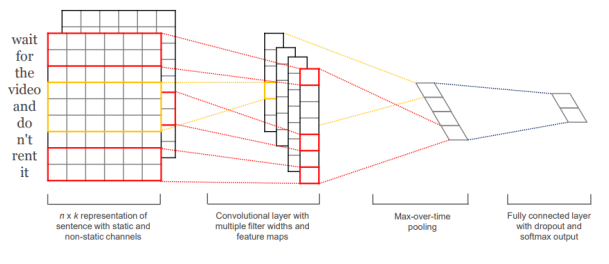
\includegraphics[width=0.6\linewidth]{images/cnn_embedding.PNG}}
 	\caption[تولید بازنمایی متن با استفاده از شبکه
 	\lr{CNN}]{تولید بازنمایی متن با استفاده از شبکه
  \lr{CNN}\cite{kim-2014-convolutional}	
 }
 	\label{cnn-embedding}
 \end{figure}
 \item کدگذاری
 \lr{BERT}
 
 
 مدل 
  \lr{BERT} \cite{devlin-etal-2019-bert}
در سال ۲۰۱۹ توسط گوگل معرفی شد.
\lr{BERT}
 یک مدل از پیش آموزش دیده برای مسائل پردازش زبان طبیعی می‌باشد. از این مدل برای تولید بازنمایی متن با کیفیت بالا می‌توان استفاده کرد. به دلیل اینکه شبکه  \lr{BERT} بر روی حجم بسیار داده آموزش دیده، بازنمایی بهتری از کلمه تولید می‌کند. همچنین با آموزش مجدد لایه آخر، برای وظایف متفاوت قابل استفاده است. مدل \lr{BERT} مبتنی بر ترنسفورمر و شامل رمزگذار دو طرفه عمیق می‌باشد.
 
 
 انواع دیگری از مدل‌های مبتنی بر
  \lr{BERT}
  نیز معرفی شدند. مدل 
 \lr{RoBERTa}\cite{liu2019roberta}
 با الگوگیری از مدل
 \lr{BERT}
 آموزش دیده است. تفاوت اصلی 
 \lr{RoBERTa}
 با
 \lr{BERT}
 در ابرپارامترهای استفاده شده است. در \lr{RoBERTa}
 اندازه دسته و نرخ یادگیری بزرگ‌تر می‌باشد. برخلاف
 \lr{BERT}
  در آموزش اولیه
 \lr{RoBERTa}
از مسئله
\lr{next-sentence prediction}
استفاده نمی‌شود. مدل
  \lr{BERTweet}\cite{bertweet}
  با روش آموزشی 
  \lr{RoBERTa}
بر داده‌های توییتر انگلیسی آموزش دیده است.  \lr{DEBERTA}\cite{liu2019roberta}
مدل
 \lr{BERT}
 و
 \lr{RoBERTa}
را با کمک توجه از هم گسسته، بهبود می‌بخشد.
\lr{XLM-RoBERTa}\cite{conneau2019unsupervised}
یک مدل چندزبانه است که بر داده‌های
\lr{CommonCrawl}
آموزش دیده است. 

\end{enumerate}

\section{یادگیری ماشین}
یادگیری ماشین
\LTRfootnote{\lr{Machine Learning}}
یکی از شاخە‌های مهم هوش مصنوعی می‌باشد. در این روش هدف یادگیری یک مدل ریاضی با استفاده از دادە‌های موجود به جای تعیین صریح قوانین در مسئله می‌باشد. بنابراین از الگوریتم‌هایی برای یادگیری الگوها و هم بستگی‌های موجود در داده‌ها استفاده می‌شود. در نهایت با استفاده از الگوهای به دست آمده یک مدل ریاضی تعریف می‌شود که از آن برای تصمیم گیری و پیشبینی استفاده می‌شود. هر چه به دادە‌های بیشتری دسترسی داشته باشیم، الگوهای بهتر و مطمئن‌تری از دادە‌ها استخراج کرده و بنابراین پیشبینی‌های دقیق‌تری خواهیم داشت.


\section{یادگیری عمیق}
یادگیری عمیق
\LTRfootnote{\lr{Deep Learning}}
شاخە‌ای از یادگیری ماشین است که مبتنی بر شبکە‌های عصبی مصنوعی
\LTRfootnote{\lr{Artificial Neural Networks}}
می‌باشد. فرآیند یادگیری، عمیق نامیده می‌شود چرا که از چندین نورون ورودی و خروجی و چندین لایه پنهان ساخته شده است.

در حالی که الگوریتم‌های یادگیری ماشین قادر هستند بسیاری از مسائل پیچیده را حل کنند، اما همچنان در برخورد با دادە‌های غیرساختاری از جمله متن، عکس و فیلم عملکرد ضعیفی دارند. روش‌های یادگیری عمیق با استفاده از شبکه‌های عصبی عمیق (که یک نوع معماری الهام گرفته از مغر انسان می‌باشد)، این مشکل را حل می‌کنند. هر لایه از شبکه عمیق ویژگی‌هایی از دادە‌های ورودی استخراج می‌کند که در نهایت می‌توان توسط ویژگی‌های استخراج شده، مسئله مورد نظر را حل کرد. اطلاعات ورودی از طریق لایە‌ها به
جلو حرکت می‌کند. 
\iffalse
در شکل
\ref{ann}
معماری یک شبکه عصبی عمیق نمایش داده شده است. در این شکل لایه ورودی، لایە‌های پنهان و لایه خروجی نیز نمایش داده شده است.

\begin{figure}[H]
	\center{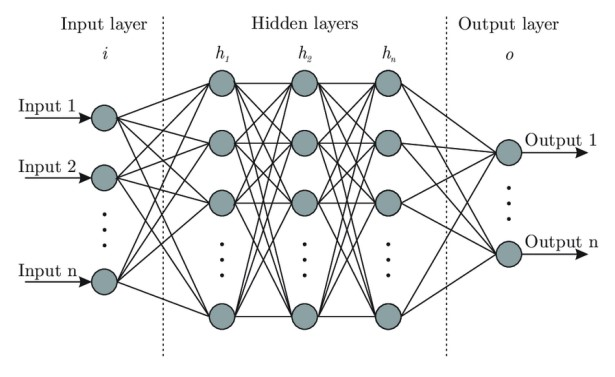
\includegraphics[width=0.5\linewidth]{images/ANN.jpg}}
	\caption{نمونه‌ای از شبکه عصبی عمیق}
	\label{ann}
\end{figure}
\fi

\section{شبکه‌های عصبی همگشتی}
شبکه‌های عصبی بازگشتی
\LTRfootnote{\lr{Recurrent Neural Network (RNN)}}
نوعی از شبکه عصبی مصنوعی است که در تشخیص گفتار، پردازش زبان طبیعی، پردازش دادە‌های ترتیبی
\LTRfootnote{\lr{Sequential Data}} 
و داده‌های سری زمانی
\LTRfootnote{\lr{Time Series}}
مورد استفاده قرار می‌گیرد. معماری این شبکه به گونە‌ای است که امکان ذخیره اطلاعات قبلی را در خود فراهم می‌کند. در بسیاری از شبکە‌های عمیق مانند شبکه عصبی پیشخور
\LTRfootnote{\lr{Feedforward Neural Network}}
دادە‌ها در یک جهت حرکت می‌کنند. یعنی از لایه ورودی به لایە‌های پنهان و سپس به سمت لایە خروجی حرکت می‌کنند و دادە‌های قبلی به حافطه سپرده نمی‌شوند. در حالی که شبکە‌های عصبی بازگشتی یک لایه بازخورد دارند که خروجی شبکه به همراه ورودی جدید، به شبکه وارد می‌شوند. این شبکه‌ها اطلاعات مربوط به ورودی قبلی را برای تاثیر بر روی ورودی و خروجی فعلی در حافظه خود ذخیره می‌کنند. در حالی که در شبکە‌های عصبی عمیق خروجی‌های مختلف از یکدیگر مستقل هستند، خروجی شبکه عصبی بازگشتی علاوه بر ورودی فعلی به عناصر قبلی توالی نیز وابسته است.

مشکل اصلی شبکە عصبی بازگشتی حافظه کوتاه مدت آن است. در بلند مدت این شبکه توانایی نگهداشتن اطلاعاتی که در گام‌های زمانی بسیار قبل‌تر به عنوان ورودی به شبکه داده شدە است را ندارد. علت این مشکل پدیده محو شدگی گرادیان
\LTRfootnote{\lr{Vanishing Gradient}}
می‌باشد. این پدیده بیان می‌کند در فرآیند بازگشت خطا به عقب
\LTRfootnote{\lr{Backpropagation}}
زمانی که به ابتدا شبکه می‌رسیم، گرادیان به تدریج کوچک می‌شود. در نتیجه تغییرات وزن بسیار کند و ناچیز می‌شود و
به عبارت دیگر آموزش کند می‌شود. این مسئله معمولا به خاطر عمق زیاد شبکه اتفاق می‌افتد. معماری‌های دیگری از جمله  \lr{LSTM} 
\cite{6795963}
و \lr{GRU} 
\cite{69e088c8129341ac89810907fe6b1bfe}
برای رفع این مشکل پیشنهاد شده است. 

ویژگی متمایز \lr{LSTM}
\LTRfootnote{\lr{Long Short-Term Memory}}
 قابلیت یادگیری وابستگی بلند مدت است که توسط شبکە‌های عصبی بازگشتی امکان پذیر نبود. شبکه عصبی بازگشتی تنها قادر به یادگیری تعداد محدودی از وابستگی‌های کوتاه مدت بود. برخلاف شبکه عصبی بازگشنی که در آن محتوا در هر گام از ابتدا بازنویسی می‌شود، در معماری \lr{LSTM} شبکه قادر است در یک گام زمانی محتوا حافظه را بدون تغییر به گام بعدی منتقل کند. به عنوان مثال اگر در گام‌های ابتدایی شبکه اطلاعات مهمی را تشخیص دهد، می‌تواند آن را برای گام‌های طولانی بدون تغییر در حافظه خود ذخیره کند.

معماری \lr{GRU} 
\LTRfootnote{\lr{Gated Recurrent Unit (GRU)}}
در سال ۲۰۱۴ معرفی شد. معماری \lr{GRU} نسخه ساده شده \lr{LSTM} می‌باشد. \lr{GRU} علاوه بر رفع مشکل محو شدگی گرادیان در شبکە عصبی بازگشتی، سربار محاسباتی \lr{LSTM} را نیز کاهش می‌دهد. همچنین با کم کردن تعداد دروازە‌ها، سرعت محاسبات را افزایش داده است.
\section{ساز و کار توجه
}\label{attention}
هدف استفاده از ساز و کار توجه
\LTRfootnote{\lr{Attention}}
بازیابی اطلاعات از بردارهای زمینه
\LTRfootnote{\lr{Context Vector}}
\lr{${y_j}$}
در رابطه با بردار پرس‌وجو
\LTRfootnote{\lr{Query Vector}}
\lr{$x$}
می‌باشد. ساز و کار توجه ابتدا امتیاز 
\lr{$\alpha_j$}
را بین بردار پرس‌وجو 
\lr{$x$}
و بردار زمینه
\lr{$y_j$}
محاسبه می‌کند.
\begin{equation}
	a_j = Score(x, y_j)
\end{equation}
\begin{equation}
	\alpha_j = \frac{exp(a_j)}{\sum_{k} exp(a_k)}
\end{equation}
خروجی لایه توجه میانگین وزن‌دار امتیاز 
\lr{$\alpha_j$}
به ازای بردار‌های زمینه می‌باشد. محاسبات انجام شده مشابه لایه 
\lr{softmax}
است. اگر بردار پرس‌وجو
\lr{$x$}
مجموعه‌ای از بردار زمینه
\lr{$\{y_j\}$}
باشد، امتیاز به دست آمده از معادله
\ref{self}
توجه به خود\LTRfootnote{\lr{self-attention}}
نامیده می‌شود.
\begin{equation}\label{self}
	Att_{x \to \{y_j\}} = \sum_{j} \alpha_jy_j
\end{equation}


\section{ترنسفورمر}
ترنسفورمر
\cite{NIPS2017_3f5ee243}
، جدیدترین معماری معرفی شده برای مسائل پردازش زبان طبیعی می‌باشد. این معماری
در سال ۲۰۱۷ معرفی شد. ترنسفورمرها با استفاده از مکانیزم توجه، امکان پردازش موازی دادە‌ها را فراهم می‌کنند. با استفاده از ترنسفورمرها برای هر کلمه می‌توان بردار بازنمایی تولید کرد. همچنین به دلیل آموزش موازی، سرعت آموزش نیز بهبود قابل توجهی پیدا می‌کند. ترنسفورمرها این قابلیت را برای ما فراهم می‌کند که به جای پردازش دنباله ورودی از ابتدا تا انتها، تنها به قسمت‌های مهم توجه کنیم. این مدل ها معمولا بر روی حجم بالایی از دادە‌ها از پیش آموزش می‌بینند
\LTRfootnote{Pre-train}.

مدل‌های زبانی بزرگ
\LTRfootnote{\lr{Large Language Models (LLMs)}}
دسته‌ای از مدل‌های زبانی هستند که توانایی درک و تولید متنی شبیه انسان را دارند. این مدل‌ها معمولاً شامل میلیون‌ها تا میلیاردها پارامتر قابل آموزش می‌باشند. برخی از آن‌ها با معماری مبتنی بر ترنسفورمرها ساخته شده‌اند.
\lr{LLMs}
ها بر روی میلیون‌ها داده آموزش دیده‌اند تا بتوانند تا بتوانند زبان انسان و انواع دیگر داده‌های پیچیده را تفسیر کنند. برخی از معروف‌ترین مدل‌های زبانی بزرگ شامل
\lr{GPT-3}،
\lr{LLaMA}\cite{touvron2023llama}
و 
\lr{Orca}\cite{orca-mini-v3-7b}
می‌باشند. 
\lr{Orca}
یک نمونه از مدل زبانی کوچک است که در دو نسخه 7 میلیارد و 13 میلیارد پارامتری عرضه شده است. این مدل با 
\lr{fine-tuning}
مدل 
\lr{LLaMA}
بر داده‌های مصنوعی با کیفیت بالا ایجاد شده است.

\section{مهندسی پرامپت}
پرامپت یک دستور متنی است که وظیفه‌ مدل را توصیف می‌کند. جدول
\ref{prompt-example}
نمونه‌‌ای از دستور متنی برای رده‌بندی در مسئله تحلیل احساسات را نشان می‌دهد (بخش‌های مختلف پرامپت نیز مشخص شده است).
\begin{table}[h!]
	\centering
	\caption{نمونه پرامپت برای مسئله تحلیل احساسات	\label{prompt-example}}
	\begin{tabular}{c c  c}
		
		دستورالعمل &  ورودی & خروجی
		\\
		\hline
		
		\lr{Classify the text into neutral, negative, or positive.}
		& \lr{Text: I think the food was okay.} 
		& \lr{Sentiment:}
	\end{tabular}

\end{table}

مهندسی پرامپت
\LTRfootnote{\lr{Prompt ٍEngineering}}
توسعه و بهینه‌سازی پرامپت برای استفاده کارآمد از مدل‌های زبانی بزرگ است. این مهارت شامل طراحی یک ورودی (دستورالعمل) مناسب برای 
\lr{LLMs} 
می‌باشد به گونه‌ای که مدل بتواند بهترین خروجی را تولید کند. مهندسی پرامپت با یادگیری درون متنی
\LTRfootnote{In-context learning}
معنا پیدا می‌کند. منظور از یادگیری درون متنی این است که مدل توانایی یادگیری موقت از پرامپت را داشته باشد. برای طراحی یک پرامپت کارآمد رویکردهای متفاوتی وجود دارد که در ادامه معروف‌ترین رویکردها را معرفی می‌کنیم
\LTRfootnote{\href{https://www.promptingguide.ai/}{https://www.promptingguide.ai/}}.

\begin{enumerate}
	\item رویکرد \lr{Zero-Shot}: 
در این رویکرد فقط یک دستورالعمل به مدل داده می‌شود (مشابه جدول 
\ref{prompt-example}). 
	\item رویکرد \lr{Chain of thought}:
	این رویکرد توانایی استدلال پیچیده را از طریق استدلال میانی برای مدل فراهم می‌کند. اضافه کردن 
	\lr{"Let's think step by step"}
	به انتهای متن یکی از معمول‌ترین دستورالعمل‌های این تکنیک به حساب می‌آید.

	\item رویکرد \lr{Few-Shot}:
	در این رویکرد علاوه بر دستورالعمل برای انجام مسئله تعریف شده، تعدادی مثال‌ از ورودی و خروجی مطلوب نیز در پرامپت گنجانده می‌شود. 
\end{enumerate}

\section{جستجو پارامترها}
مدل‌های یادگیری ماشین شامل پارامترها و فراپارامترهایی
\LTRfootnote{Hyperparameter}
 هستند که می‌توانند مقادیر مختلفی داشته باشند. انتخاب مقادیر این پارامترها همواره یکی از چالش‌های یادگیری به حساب می‌آید. روش‌های مختلفی برای انتخاب پارامترها وجود دارد. ساده‌ترین رویکرد برای انتخاب پارامترها  جستجو تصادفی
\LTRfootnote{Random Search}
می‌باشد. در این رویکرد برای هر یک از پارامترها یک فضا جستجو تعریف می‌شود. در هر بار اجرا به صورت کاملا تصادفی برای هر پارامتر مقداری انتخاب می‌شود. این روش لزوما بهترین مقادیر را هر پارامتر را به دست نمی‌آورد.
روش جستجو شبکه‌ای 
\LTRfootnote{Grid Search}
تمام حالت‌های ممکن فضا تعریف شده را جستجو می‌کند. مشکل اصلی این روش نفرین ابعاد
\LTRfootnote{Curse of Dimensionality}
می‌باشد. به این معنی که هر چه ابعاد فضا جستجو بزرگ‌تر شود، پیچیدگی زمانی به صورت نمایی افزایش پیدا خواهد کرد.


برخی از روش‌های بهینە‌سازی فراپارامترها در هر بار انتخاب فراپارامترها برای آزمایش بعدی، از اطلاعات ترکیب قبلی نیز استفاده می‌کنند. این روش‌های انتخاب تطبیقی
\LTRfootnote{Adaptive Selection}،
با انتخاب فراپارامترهایی که احتمال موفقیت‌شان بیشتر است، سرعت جستجو را به طور قابل توجهی افزایش می‌دهند. یکی از ابزارهای معرفی شده در این روش،
\lr{Optuna}\cite{10.1145/3292500.3330701}
می‌باشد. این رویکرد فضا جستجو پارامترها را به صورت پویا ساختاردهی می‌کند. برای انتخاب هر نمونه از فصا جستجو از الگوریتم
\lr{TPE}\LTRfootnote{Tree-Structured Parzen Estimator}
که بر مبنای بهینه‌سازی
\lr{Bayesian}
است استفاده می‌کند. همچنین 
\lr{Optuna}
با قابلیت توقف زود هنگام
\LTRfootnote{Early Stopping}
با استفاده از روش‌های 
\lr{Pruning}
احتمال رسیدن به پارامترهای بهینه در کوتاه‌ترین زمان ممکن را افزایش می‌دهد.

\section{جمع بندی}
در این فصل، ابتدا شبکه اجتماعی و پردازش زبان طبیعی معرفی شد. سپس مکانیزم‌های تعبیه کلمات که یکی از مهم‌ترین روش‌های کار با متن است مورد بررسی قرار گرفت. همچنین مفاهیم یادگیری عمیق، مهندسی پرامپت و روش‌های جستجو به عنوان مهم‌ترین رویکرد حل مسئله بررسی شد. آشنایی با این مفاهیم، درک مسئله تشخیص موضع را آسان تر می‌کند.
	



%!TeX root=main.tex
\chapter{مروری بر کار‌های مرتبط}
\thispagestyle{empty}

در سال‌های اخیر تحقیقات در تشخیص موضع افزایش چشم‌گیری داشته است (شکل~\ref{StancePublicationPerYear}). در این بخش ابتدا رقابت‌های برگزار شده در زمینه تشخیص موضع را مورد بررسی قرار می‌دهیم. سپس تعدادی از مجموعه دادە‌های معرفی شده را بررسی می‌کنیم. در ادامه رویکردهای معرفی شده برای تشخیص موضع را معرفی می‌کنیم.

\begin{figure}[H]
	\center{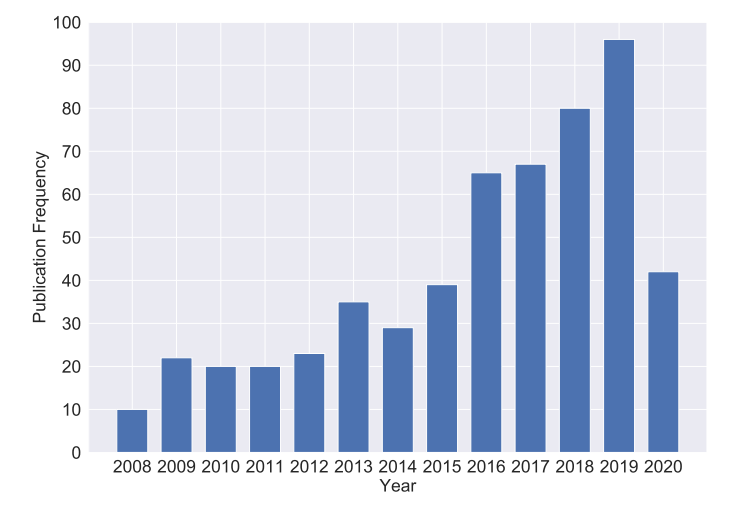
\includegraphics[width=0.7\linewidth]{images/StancePublicationPerYear.PNG}}
	\caption[نمودار تعداد مقالات چاپ شده در رابطه با تشخیص موضع به تفکیک سال]
	{نمودار تعداد مقالات چاپ شده در رابطه با تشخیص موضع به تفکیک سال. جستجو براساس
		کلمات کلیدی «تشخیص موضع»، «پیش بینی موضع» و «ردە‌بندی موضع» انجام شده است \cite{ALDAYEL2021102597}.}

	\label{StancePublicationPerYear}
\end{figure}

\section{رقابت‌های برگزار شده در مسئله تشخیص موضع}
با بررسی منابع موجود، مشخص شد تا کنون شش رقابت در رابطه با مسئله تشخیص موضع برگزار شده است. در این رقابت‌ها مجموعە دادە‌های جدید و مدل‌های مرتبط با آن‌ها معرفی می‌شوند. بنابراین برگزاری چنین رویدادهایی نقش مهمی در رشد و تقویت تحقیقات در تشخیص موضع دارند \cite{10.1145/3369026}. مهم‌ترین رویدادهای برگزار شده به شرح زیر است.
\subsection{رویداد
	\lr{SemEval-2016}}
اولین رقابت برگزار شده برای مسئله تشخیص موضع، رقابت 
\href{https://alt.qcri.org/semeval2016/task6/}{\lr{SEMEval2016:Task6}}\LTRfootnote{\href{{https://alt.qcri.org/semeval2016/task6/}}{{https://alt.qcri.org/semeval2016/task6/}}}
می‌باشد. در این رقابت چندین مسئله تعریف شده که مسئله ششم مرتبط با تشخیص موضع می‌باشد. این رقابت شامل دو زیر مسئله است \cite{mohammad-etal-2016-semeval}.

\begin{enumerate}
	\item تشخیص موضع با نظارت
	\LTRfootnote{\lr{Supervised Stance Detection}}
	\newline
	مجوعه داده دارای برچسب برای ۵ موضوع
	\LTRfootnote{\lr{Target}}
	 که دارای ۲۸۱۴ توییت در قسمت دادە‌های آموزشی و
	۱۲۴۹ توییت در دادە‌های ارزیابی می‌باشد.
	\item تشخیص موضع با نظارت ضعیف
	\LTRfootnote{\lr{Weakly Supervised Stance Detection}}
	\newline
	شامل حدودا ۷۸۰۰۰ توییت بدون برچسب به عنوان دادە‌های آموزشی می‌باشد. دادە‌های ارزیابی شامل ۷۰۷ توییت در رابطه با هدف دیگری می‌‌باشد.
\end{enumerate}

	در مجموع ۱۹ گروه در این رقابت شرکت کردند. شرکت کنندگان در این مسابقه از روش‌های مختلفی استفاده کردند. روش‌های استفاده شده شامل یادگیری ماشین سنتی مبتنی بر ویژگی
	\LTRfootnote{\lr{Feature-Based Machine Learning}}
	، یادگیری عمیق و یادگیری مجمع
	\LTRfootnote{\lr{Ensemble Learning}}
	می‌باشد. بهترین مدل معرفی شده برای زیر مسئله اول (تشخیص موضع با نظارت)، از	یادگیری مجمع شبکه عصبی بازگشتی 
	\lr{(RNN)} 
استفاده کرده است. در ارزیابی نهایی، این روش به مقدار
\lr{67.82\%}
برای معیار
\lr{F1-Score}
دست یافت \cite{zarrella-marsh-2016-mitre}. همچنین بهترین مدل (در قیاس با ۹ روش معرفی شده) برای زیر مسئله دوم (تشخیص موضع با نظارت ضعیف) از شبکه عصبی پیچشی 
\lr{(CNN)}
استفاده کرد که در ارزیابی پایانی مقدار
 \lr{56.28\%}
 برای معیار
 \lr{F1-Score}
 دست یافت \cite{wei-etal-2016-pkudblab}. علاوه بر این، مدل مبتنی بر شبکه عصبی پیچشی
 \lr{(CNN)}
 با مقدار
  \lr{67.33\%}
  برای معیار
   \lr{F1-Score}
جایگاه دوم را برای زیر مسئله اول کسب کرد. مدل پایە‌ای که توسط طراحان مسابقه توسعه یافته از روش 
\lr{SVM}
استفاده کرده است. در ارزیابی انتهایی به مقدار
 \lr{68.98\%}
 برای معیار
\lr{F1-Score}
دست یافت. این بالاترین مقدار در بین همه شرکت کنندگان در رویداد می‌باشد.
 
%\iffalse
\subsection{رویداد
	\lr{NLPCC-ICCPOL-2016}}

رقابت
\lr{NLPCC-ICCPOL-2016}
تشخیص موضع بر روی وبلاگ‌های کوتاه به زبان چینی است \cite{10.1007/978-3-319-50496-4_85}. در این
رقابت چندین مسئله تعریف شده که مسئله چهارم مرتبط با تشخیص موضع می‌باشد. در این رقابت نیز دو زیر مسئله مشابه با
\lr{SemEval-2016}
 تعریف شد.
 
 \begin{enumerate}
 	\item تشخیص موضع با نظارت
 	
 	حدود ۴۰۰۰ وبلاگ کوتاه به صورت دستی
 		\LTRfootnote{\lr{Manual}}
 	 برای ۵ موضوع حاشیە نویسی شده است. موضوعات
 	شامل
 	 \lr{SE iPhone}،
 	  ترقی در جشنواره بهار، عملیات ضد تروریستی روسیه در سوریه، سیاست دو فرزند و ممنوعیت موتورسیکلت و محدودیت وسایل نقلیه الکترونیکی در شنژن می‌باشد. از این میان
 	\lr{75\%}
 	 دادە‌ها برای آموزش و مابقی دادە‌ها برای ارزیابی استفاده می‌شوند.
 	
 	\item 
 	تشخیص موضع بدون ناظر
	\LTRfootnote{\lr{Unsupervised Stance Detection}}
	
	در این روش از مجموعه داده بدون برچسب برای آموزش بدون ناظر استفاده می‌شود. دادە‌های این قسمت شامل ۲۴۰۰ وبلاگ کوتاه بدون برچسب است. این دادە‌ها شامل دو موضوع موارد غذایی اصلاح شده ژنتیکی و آزمایش‌های هستە‌ای کره شمالی می‌باشند.
 \end{enumerate}

در این رقابت شانزده تیم در زیر مسئله اول (تشخیص موضع با نظارت) و پنج تیم در زیر مسئله دوم (تشخیص موضع بدون ناظر) شرکت کردند. برنده رقابت در زیر مسئله اول، یک مدل ردە بندی جداگانه برای
هر موضوع آموزش داده است. پایه مدل‌های استفاده شده 
\lr{SVM}
 و 
 \lr{Forest Random}
  هستند. بالاترین مقدار
  \lr{F1-Score}
 به دست آمده برابر با
 \lr{71.06\%}
 می‌باشد.
 
 ویژگی‌های ورودی بهترین سیستم شامل
 \lr{Unigram}،
 \lr{TF-IDF}	\LTRfootnote{\lr{Term Frequency-Inverse Document Frequency}}،
  کلمات مشابه و بردارهای بازنمایی در سطح کلمه و کاراکتر می‌‌باشد. سایر ویژگی‌های استفاده شده توسط سایر شرکت کنندگان شامل 
  \lr{Bigram}
   و واژگان شامل احساسات 
\LTRfootnote{\lr{Sentiment Lexicons}}
   می‌باشد. همچنین با بررسی نتایج شرکت کنندگان این نتیجه حاصل شد که نتیجه بهتر در مسئله تحلیل احساسات لزوما به این معنا نیست که مدل می‌تواند در مسئله تشخیص موضع نیز به نتایج خوبی دست پیدا کند. بالاترین نتیجه کسب شده برای زیر مسئله دوم (تشخیص موضع بدون ناظر) برابر با
    \lr{46.87\%} 
    است.
\subsection{رویداد
	\lr{IberEval-2017}}

رویداد
\lr{IberEval-2017}
مشابه با دو رویداد قبلی می‌باشد. یکی از مسائل تعریف شده در این رقابت مربوط به تشخیص موضع و تشخیص جنسیت در زبان اسپانیایی و کاتالان می‌باشد \cite{taule2017overview}.

روش‌های متداول استفاده شده توسط شرکت کنندگان شامل
\lr{SVM}
، شبکه عصبی، روش‌های یادگیری
عمیق از جمله 
\lr{LSTM}
 می‌باشد. همچنین ویژگی‌های
 \lr{ngram}
  و بازنمایی کلمات
  	\LTRfootnote{\lr{word embedding}}
   از جمله متداول‌ترین ویژگی‌های استفاده شده برای این مسئله بود.
   
   ده تیم در این رقابت شرکت کردند. بهترین مدل معرفی شده برای تشخیص موضع در زبان اسپانیایی روش
    \lr{SVM}
     با ترکیبی از چندین ویژگی مطرح شده در قسمت بالا به عنوان ورودی مدل است. این در حالی است که مدل 
     \lr{Logistic Regression}
     برای زبان کاتالان به نتیجه بهتری دست یافته است. روش‌های یادگیری عمیق نتایج خوبی در این رقابت کسب نکردە اند.
   
\subsection{رویداد
	\lr{SadriStance@EVALITA-2020}}
رویداد  
\lr{SadriStance@EVALITA-2020}
اولین رقابت برگزار شده در تشخیص موضع به زبان ایتالیایی می‌باشد.
مجموعه داده جمع‌آوری‌شده درباره موضوع جنبش
\href{https://en.wikipedia.org/wiki/Sardines_movement}{Sadrines}
در ایتالیا (سال ۲۰۱۹) می‌باشد. در مجموع ۳۲۴۲ توییت از توییتر جمع‌آوری شده است. از این میان ۱۷۷۰ توییت برچسب مخالف، ۷۸۴ توییت برچسب موافق و ۶۸۷ توییت باقی مانده برچسب بدون نظر دارند. این رقابت دو زیر مسئله را برای شرکت کنندگان تعریف می‌کند \cite{cignarella2020sardistance}.
\begin{enumerate}
	\item تشخیص موضع بر اساس متن توییت
	\LTRfootnote{\lr{Textual Stance Detection}}
	
	در این زیر مسئله شرکت کنندگان برای تشخیص موضع فقط متن توییت را در اختیار دارند.

	\item تشخیص موضع بر اساس ویژگی‌های محتوایی
	\LTRfootnote{\lr{Contextual Stance Detection}}
	
	در این حالت علاوه بر متن توییت برخی دیگر از ویژگی‌ها از جمله تعداد بازاشتراک گذاری
	\LTRfootnote{\lr{Retweets}}،
	تعداد افرادی که در روز اول انتشار توییت آن را پسندیدە‌اند نیز مورد استفاده قرار می‌گیرد. همچنین تعداد دنبال کنندگان
	\LTRfootnote{\lr{Follower}}،
	موقعیت مکانی فرد منتشر کننده توییت نیز در دسترس است. سایر اطلاعاتی که از شبکه اجتماعی توییتر از یک کاربر در درسترس می‌باشد از جمله ویژگی‌هایی است که در آموزش	مدل می‌توان از آن استفاده کرد. این ویژگی‌ها شامل
\lr{quotes}
	  و نظرات در ارتباط با توییت نیز می‌باشد.
\end{enumerate}

در این رقابت سیزده تیم در زیر مسئله اول (تشخیص موضع بر اساس متن توییت) و دوازده تیم در زیر مسئله دوم (تشخیص موضع بر اساس ویژگی‌های محتوایی) شرکت کردند. شرکت کنندگان روش‌های متنوعی را برای حل تشخیص موضع پیشنهاد دادند.
\lr{SVM}
و
\lr{Logistic Regression}
از جمله مدل‌های مبتنی بر یادگیری ماشین استفاده شده هستند. همچنین
\lr{BiLSTM}
و
\lr{CNN}
و مکنیزم توجه از جمله روش‌های یادگیری ماشین استفاده شده است. در نهایت روشی که از 
\lr{BERT} \cite{kenton2019bert}
استفاده کرده بهترین نتیجه را در مقایسه یا سایر شرکت کنندگان کسب کرده است. نایج نشان می‌دهد استفاده از ویژگی‌های کاربران در شبکە‌های اجتماعی باعث بهبود
\lr{F1-Score}
 می‌شود.

\subsection{رویداد
	\lr{VaxxStance@IberLFE-2021}}

رویداد 
\href{https://vaxxstance.github.io/}{\lr{VaxxStance@IberLFE-2021}}\LTRfootnote{\href{{https://vaxxstance.github.io/}}{{https://vaxxstance.github.io/}}}
برای تشخیص موضع بر روی دو زبان اسپانیایی و باسکی
\footnote{
باسکی زبان استفاده شده توسط مردم باسک ساکن در شمال اسپانیا و جنوب فرانسه می‌باشد. 
}
 برگزار شد \cite{agerri2021vaxxstance}.  دادە‌های جمع آوری شده برای این مسابقه، درباره موضوع واکسن کرونا در دو زبان جمع آوری شده است. در جمع‌آوری مجموعه داده دقت شده تعداد کاربرها و توییت‌ها متناسب باشد. حالتی که تعداد زیادی توییت متعلق به تعداد کمی کاربر باشد مطلوب نیست. همچون رویداد قبلی، علاوه بر متن توییت سایر ویژگی‌های مربوط به کابران در شبکه اجتماعی نیز جمع آوری شده است. برای جمع‌آوری داده از هشتک‌های مرتبط با موضوع واکسن کرونا استفاده کردند. همچنین چالش بزرگ در جمع‌آوری مجموعه داده، پیدا کردن داده با برچسب مخالف بود.در نهایت برای زبان باسکی ۱۳۸۴ توییت که در مجموع مربوط به ۲۱۰ کاربر بود جمع آوری شد. داده جمع‌آوری‌شده به زبان اسپانیایی نیز شامل ۲۶۵۲ توییت مختلف به ۱۶۷۶ کابر می‌باشد. این رقابت سه زیر مسئله را برای شرکت کنندگان تعریف می‌کند.
 
 \begin{enumerate}
 	\item زیر بخش اول
 	\lr{(Close Track)}
 	
 	در این زیر مسئله تنها مجاز به استفادە از دادە‌هایی که در رقابت در اختیار شرکت کننده قرار داده شده هستند. به عنوان مثال نمی‌توان برای آموزش بردار بازنمایی بهتر برای کلمات، از مجموعه دادە‌های	دیگر استفاده کرد. مدل‌های این زیر بخش به دو صورت آموزش می‌‌بینند. نوع اول مدل‌هایی هستند 	که برای آموزش آن‌ها تنها از دادە‌های متنی استفاده شده است. دسته دوم مدل‌هایی هستند که علاوه 	بر دادە‌های متنی، ویژگی‌های مربوط به شبکه اجتماعی توییتر را نیز در اختیار دارند.
 	\item زیر بخش دوم
 	\lr{(Open Track)}
 	
 	در این بخش بر خلاف قسمت قبل، شرکت کنندگان مجاز به استفاده از همه نوع داده هستند. هدف این است به کمک تکنیک‌های افزایش داده 
 	\lr{Data Augmentation}
 	و انتفال دانش بین دو زبان مختلف کیفیت نتایج خروجی بهبود یابد.
 	\item زیر بخش سوم
 	\lr{(Zero-shot Track)}
 	
 	در این بخش نمی‌توان از توییت‌های مربوط به زبان مبدا در آموزش مدل استفاده کرد. هدف حل تشخیص موضع با استفاده از دادە‌های شبکەهای اجتماعی و بدون استفاده از متن می‌باشد.
 \end{enumerate}
 
 در این رقابت بیست تیم ثبتنام کردند اما تنها سه تیم نتایج خود را ارسال کردند. همچنین در زیربخش  دوم و سوم تنها یک تیم شرکت کرد. نتیجه به دست آمده نشان می‌دهد مدل آموزش داده شده به زبان اسپانیایی از کیفیت بالاتری برخوردار هستند. همچنین اگر در آموزش مدل علاوه بر متن از ویژگی‌های شبکه اجتماعی استفاده شود، بهبود قابل توجه در نتایج به دست خواهد آمد. برای زیربخش اول و دوم نتایج به زبان اسپانیایی بهتر از نتایج زبان باسکی است. اما در
 زیر بخش سوم نتایج برای دو زبان به یکدیگر نزدیک است.
%\fi
\subsection{رویداد
	\lr{ClimateActivismStance@CASE-2024}}\label{sec:ClimateActivismStance}
رویداد 
	\lr{ClimateActivismStance}
	\LTRfootnote{\href{https://github.com/therealthapa/case2024-climate}{https://github.com/therealthapa/case2024-climate}}
برای تشخیص موضع و تشخیص سخنان نفرت انگیز
\LTRfootnote{\lr{Hate Speech}}
در موضوع تغییرات اقلیمی به زبان انگلیسی برگزار شد
\cite{thapa2024stance}.
داده‌های استفاده شده از توییتر جمع‌آوری شدند. این رویداد سه زیرمسئله را برای شرکت کنندگان تعریف می‌کند.
\begin{enumerate}
	\item زیر مسئله اول (تشخیص سخنان نفرت انگیز) 
	
در این زیر بخش، هدف  اصلی تشخیص وجود سخنان نفرت انگیز به ازای متن موجود می‌باشد. مسئله تعریف شده یک رده‌بند دو کلاسه می‌باشد.
	\item 
	زیر مسئله دوم (تشخیص موضوع سخنان نفرت انگیز)
	
	در این زیر بخش هدف تشخیص موضوع سخنان نفرت آمیز به ازای متن موجود می‌باشد. موضوعات شامل فردی
	\LTRfootnote{\lr{Individual}}،
	سازمانی
	\LTRfootnote{\lr{Organization}}
	و اجتماع
	\LTRfootnote{\lr{Community}}
	می‌باشد.
	\item زیر مسئله سوم (تشخیص موضع)
	
	در این بخش هدف تشخیص موضع برای متن ورودی است. موضع یکی از سه کلاس تایید، رد و بدون نظر می‌باشد.
	
\end{enumerate}

در مجموع 23 تیم در زیر مسئله اول، 18 تیم در زیر مسئله دوم و 19 تیم در زیر مسئله سوم شرکت کردند.  مدل‌های مبتنی بر 
\lr{Transformer}
نتایج بهتری کسب کردند. 
بالاترین مقدار
\lr{F1-Score}
به دست آمده برای زیر مسئله اول (تشخیص سخنان نفرت انگیز)
\lr{ 91.44\%} 
برای زیر مسئله دوم (تشخیص موضوع سخنان نفرت انگیز)
\lr{ 78.58\%} 
و برای زیر مسئله سوم (تشخیص موضع)
\lr{ 74.83\%} 
می‌باشد.
نتایج به دست آمده از این رویداد برای زیر مسئله سوم در جدول 
\ref{climate_activism_result}
قابل مشاهده است (تیم
\lr{IUST}
نیز توانست مقام سوم را در بخش تشخیص موضع کسب کند). تیم اول مسابقات مدل
\lr{bERTweet}
با طول ورودی 96 توکن را معرفی کرده است. همچنین تیم دوم مسابقات با استفاده از مهندسی پرامپت و مدل
\lr{Llama}
توانست نتایج قابل قبولی کسب کند.

 \begin{table}[ht]
 	\centering
 	\small
	\begin{figure}[H]
		\center{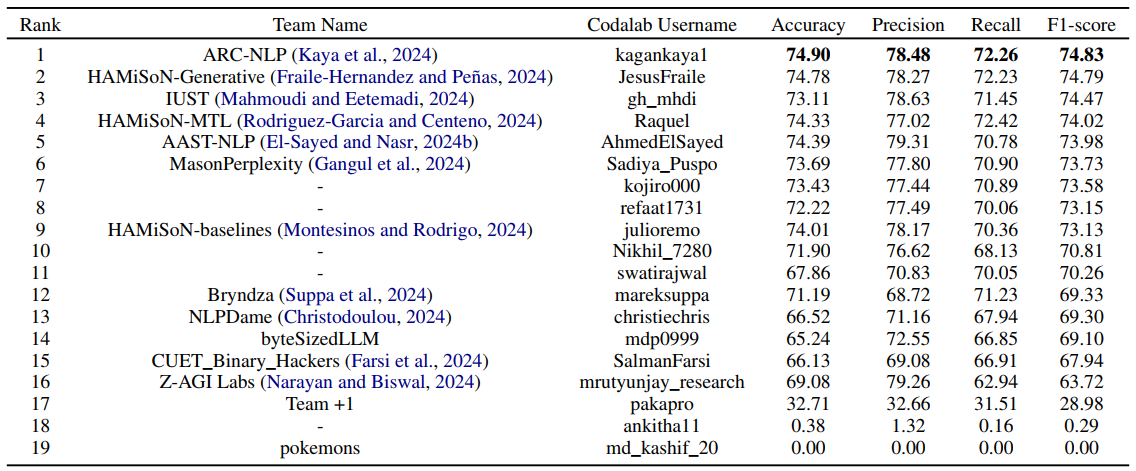
\includegraphics[width=1\linewidth]{images/Climate_Activism_result.PNG}}
	\end{figure}
 	\caption[نتایج رویداد
 	\lr{ClimateActivismStance}
 	برای زیر مسئله سوم (تشخیص موضع)]
 	{\label{climate_activism_result}  نتایج رویداد
 	\lr{ClimateActivismStance}
 	برای زیر مسئله سوم (تشخیص موضع)
 	\cite{thapa2024stance}
 }
 \end{table}

\section{مجموعه داده‌های مسئله تشخیص موضع}
با وجود اینکه تشخیص موضع، یک مسئله نوظهور و جدید است، اخیرا تلاش‌های قابل توجهی برای جمع آوری مجموعه داده در این حوزه انجام شده است. اغلب مجموعه دادە‌ها به صورت عمومی در دسترس تمام افراد قرار دارد. مجموعه دادە‌های جمع‌آوری‌شده معمولا از متن‌های مختلف از جمله توییت‌ها، پست‌ها در سایت‌های آنلاین، مقالات خبری و یا نظرات درباره خبرها جمع‌آوری شدە‌اند. 

مجوعه داده
\lr{Multi-Target}\cite{sobhani-etal-2017-dataset}
شامل توییت‌هایی در مورد چهار تن از نامزد‌های انتخابات ریاست جمهوری
آمریکا است. این افراد شامل دونالد ترامپ، هیلاری کلینتون، تد کروز و برنی سندرز می‌باشند. هر موضوع شامل دو تن از کاندیدا ریاست جمهوری می‌باشد (جدول
\ref{dataset-multitarget}). بنابراین برای هر موضوع دو برچسب موجود است (به ازای هر کاندید موضع توییت مشخص می‌شود). مجموعه داده شامل ۴۴۵۵ توییت که به صورت دستی برچسب زده شده است. این مجموعه داده، اولین مجموعه داده معرفی شده به صورت چند موضوعی
\lr{(Target-Multi)}
می‌باشد.
\begin{table}[ht]
	\centering
	\small
	\caption[توزیع نمونە ها در مجموعه داده
	\lr{Multi-Target}]{\label{dataset-multitarget} توزیع نمونە ها در مجموعه داده
		\lr{Multi-Target}\cite{sobhani-etal-2017-dataset}}
	
	\begin{figure}[H]
		\center{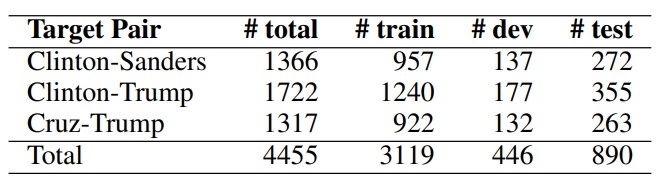
\includegraphics[width=0.5\linewidth]{images/Multi_target.jpg}}
	\end{figure}
	
\end{table}
مجموعه داده
\lr{WT-WT}\LTRfootnote{Will-They-Won’t-They}\cite{conforti-etal-2020-will}
جمع‌آوری شده به زبان انگلیسی شامل ۵۱۲۸۴ توییت می‌باشد. مجموعه داده جهت تشخیص موضع شایعه در بازارهای مالی جمع آوری شده است. توییت‌های جمع‌آوری شده درباره بحث‌های صورت گرفته در خصوص واگذاری یک شرکت به شرکت دیگر و یا تجمیع دو شرکت است.

مجموعه داده
\lr{X-Stance}\cite{vamvas2020xstance}
شامل 67000 داده در ارتباط با کاندیدا ریاست جمهوری سوییس به چهار زبان انگلیسی، آلمانی، فرانسوی و ایتالیایی می‌باشد. مجوعه داده
\lr{P-Stance}\cite{li-etal-2021-p}
شامل ۲۱۵۷۴ توییت به زبان انگلیسی درباره سه کاندید ریاست جمهوری آمریکا شامل دونالد ترامپ، جوبایدن و برنی سندز می‌باشد. مجموعه دادە‌های قبلی جمع آوری شده از توییتر، اغلب شامل دادە‌های بسیار کمی بودند. همین موضوع انگیزە ای برای جمع آوری مجموعه داده
 
\lr{P-Stance}
شد. مجموعه داده
\lr{VAST}\cite{Allaway2020Zero}
برای تشخیص موضع بدون داده آموزشی 
\LTRfootnote{Zero-Shot}
یا با داده آموزشی کم
\LTRfootnote{Few-Shot}
از نظرات موجود در تیویورک تایم جمع آوری شده است. این مجموعه داده شامل موضوعات متنوعی است. از هر موضوع تعداد داده کمی در مجموعه داده
موجود است. 

تا به اینجا معرفی مختصر بر تعدادی از مجوعه‌ داده‌های تشخیص موضع داشتیم. در ادامه به معرفی دقیق‌تر دو مجموعه داده \lr{SemEval-2016} و \lr{ClimaConvo} در این پژوهش می‌پردازیم.

\subsection{مجموعه داده
	\lr{SemEval-2016}
}

از معروف ترین مجموعه دادگان به زبان انگلیسی برای مسئله تشخیص موضع که در پژوهش های زیادی مورد استفاده قرار گرفته، مجموعه داده
 \lr{SemEval}
  است. این مجموعه داده برای اولین بار در رویداد
  \lr{SemEval2016}
برای دو زیر مسئله تشخیص موضع با نظارت و تشخیص موضع با نظارت ضعیف معرفی شد. این مجموعه داده از شش موضوع شامل انکار وجود خدا
\LTRfootnote{\lr{Atheism}}،
نگرانی از تغییرات آب و هوایی
\LTRfootnote{\lr{Climate Change is Concern}}،
جنبش فمینیسم
\LTRfootnote{\lr{Feminist Movement}}،
هیلاری کلینتون
\LTRfootnote{\lr{Hillary Clinton}}،
قانونی شدن سقط جنین
\LTRfootnote{\lr{Legalization of Abortion}}
و دونالد ترامپ
\LTRfootnote{\lr{Donald Trump}}
تشکیل شده است.

مجموعه دادگان
\lr{SemEval}
اولین مجموعه داده جمع‌آوری‌شده از پست‌های توییتر برای موضوع خاص
در مسئله تشخیص موضع است. این مجموعه داده علاوه بر برچسب تشخیص موضع، شامل برچسب تحلیل احساسات نیز می‌باشد. مجموعه داده توسط افراد و به صورت دستی، طبق پروتکل خاص برچسب گذاری شده است. چند نمونه از دادە‌های موجود در مجموعه داده در جدول~\ref{dataset-semeval} نشان داده شده است.


\begin{table}[ht]
	\centering
	\small
	\caption[چند نمونه از دادە‌های مجموعه داده
	\lr{SemEval}]{\label{dataset-semeval}  چند نمونه از دادە‌های مجموعه داده
		\lr{SemEval}\cite{mohammad-etal-2016-semeval}}
	
	\begin{figure}[H]
		\center{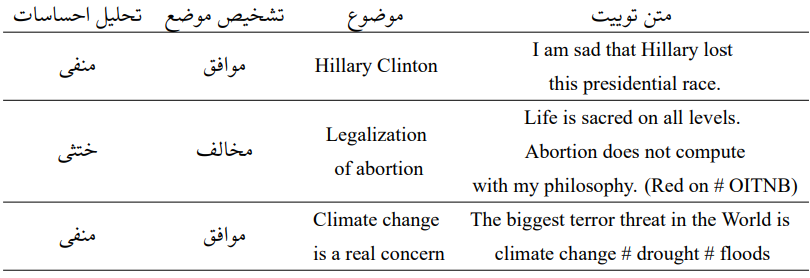
\includegraphics[width=0.9\linewidth]{images/semeval_example.PNG}}
	\end{figure}
	
\end{table}

برای جمع‌آوری مجموعه داده هشتک‌های خاصی در توییتر سرچ شدند. سپس تنها توییت‌هایی که در انتها آن‌ها هشتک وجود داشت نگه داشته و مابقی توییت‌ها حذف شدند. همچنین گاهی از روی هشتک موجود، می‌توان موضع را تشخیص داد. بنابراین هشتک‌های توییت‌ها نیز حذف شدند. برای جمع‌آوری دادە‌ها قوانین خاصی در نظر گرفته شد. به عنوان مثال اینکه (۱) توییت‌ها توسط مردم آمریکا قابل فهم باشد. (۲) برای
هر موضوع خاص از هر سه کلاس موافق، مخالف و بدون نظر داده به اندازه کافی وجود داشته باشد. (۳) مجموعه داده بهتر است شامل توییت‌هایی باشد که بدون اشاره مستقیم به هدف، موضع خود را نسبت به هدف بیان کند. (۴) مجموعه داده باید شامل دادە‌هایی باشد که هدف مورد نظر توییت با موضوع انتخابی توسط ما متفاوت باشد.
در نهایت مجموعه دادە ای شامل ۴۸۷۰ داده جمع آوری شد. توزیع نمونە ها بر اساس موضوعات در جدول
\ref{dataset-semeval-statistic}
قابل مشاهده است .


\begin{table}[ht]
	\centering
	\small
	\caption[چند نمونه از دادە‌های مجموعه داده
	\lr{ClimaConvo}]{\label{dataset-semeval-statistic}  توزیع نمونە‌ها در مجموعه داده
	\lr{SemEval}\cite{mohammad-etal-2016-semeval}}
	
	\begin{figure}[H]
		\center{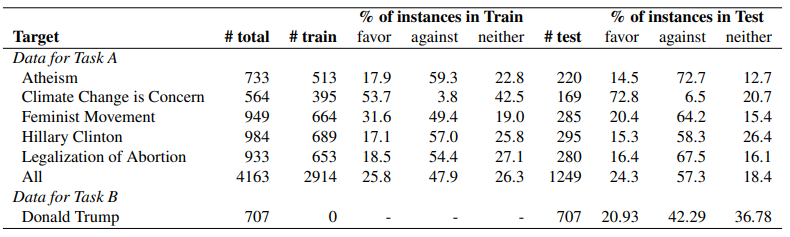
\includegraphics[width=0.9\linewidth]{images/SemEvalStatistic.PNG}}
	\end{figure}
	
\end{table}
\subsection{مجموعه داده
	\lr{ClimaConvo}
}\label{sec:datasetClimaConvo}
یکی از جدید‌ترین مجموعه داده‌های معرفی شده برای تشخیص موضع
\lr{ClimaConvo} \cite{shiwakoti2024analyzing}
می‌باشد. این مجموعه داده در رویداد
\lr{ClimateActivismStance}\cite{thapa2024stance}
معرفی و استفاده شده است. این مجموعه داده شامل حدود 15 هزار توییت در موضوع تغییرات اقلیمی می‌باشد. شش مسئله متفاوت پردازش زبان طبیعی بر روی این مجموعه داده تعریف شده است. داده‌های این مجموعه داده، مربوط به توییت‌های سال 2022 می‌باشد. برای جمع‌آوری مجموعه داده، توییت‌های شامل هشتک‌های مربوط به تغییرات اقلیمی جمع‌آوری شدند.  به عنوان مثال
\lr{\#climatecrisis, \#climatechange, \#ClimateEmergency, \#ClimateTalk, \#globalwarming}
نمونه‌ای از هشتگ‌های استفاده شده برای جمع‌آوری داده می‌باشد.
%\subsection{سایر مجموعه داده‌های تشخیص موضع}
\begin{table}[ht]
	\centering
	\small
	\caption[چند نمونه از دادە‌های مجموعه داده
	\lr{ClimaConvo}]{\label{dataset-climate-convo}  چند نمونه از دادە‌های مجموعه داده
		\lr{ClimaConvo}\cite{shiwakoti2024analyzing}}
	
	\begin{figure}[H]
		\center{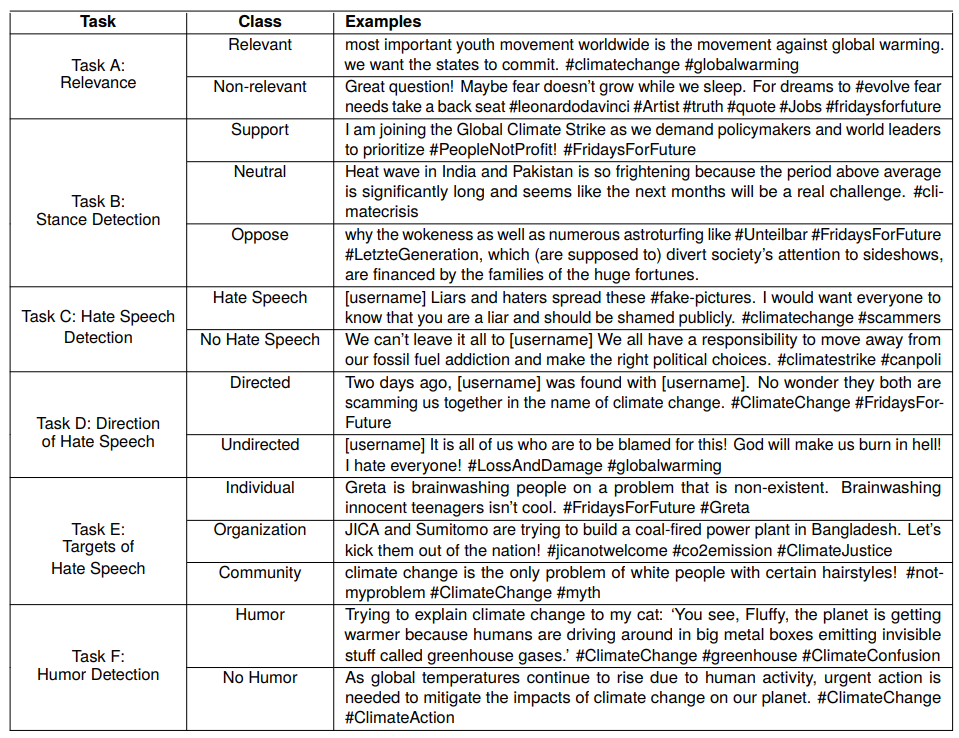
\includegraphics[width=1\linewidth]{images/ClimaConvo_Example.PNG}}
	\end{figure}
	
\end{table}


\section{پژوهش‌های انجام شده در مسئله تشخیص موضع}
همان‌طور که در بخش
\ref{sec:stance-detection-level}
اشاره شد، تشخیص موضع در سطوح متفاوتی تعریف می‌شود. شکل
\ref{stance_modeling_level}
شامل مروری جامع بر روش‌های ارائه شده در هر سطح می‌باشد. این شکل به صورت طبقه‌بندی شده ویژگی‌های مورد استفاده برای تشخیص موضع را نشان می‌دهد. در ادامه مروری بر روش‌های رده‌بندی در سطح محتوا
\LTRfootnote{Content}
 خواهیم داشت. رویکردهای ارائه شده را به دو دسته‌بندی کلی می‌توان تقسیم کرد. در ادامه پژوهش‌های هر بخش به طور مختصر معرفی خواهد شد.
\begin{figure}
	\center{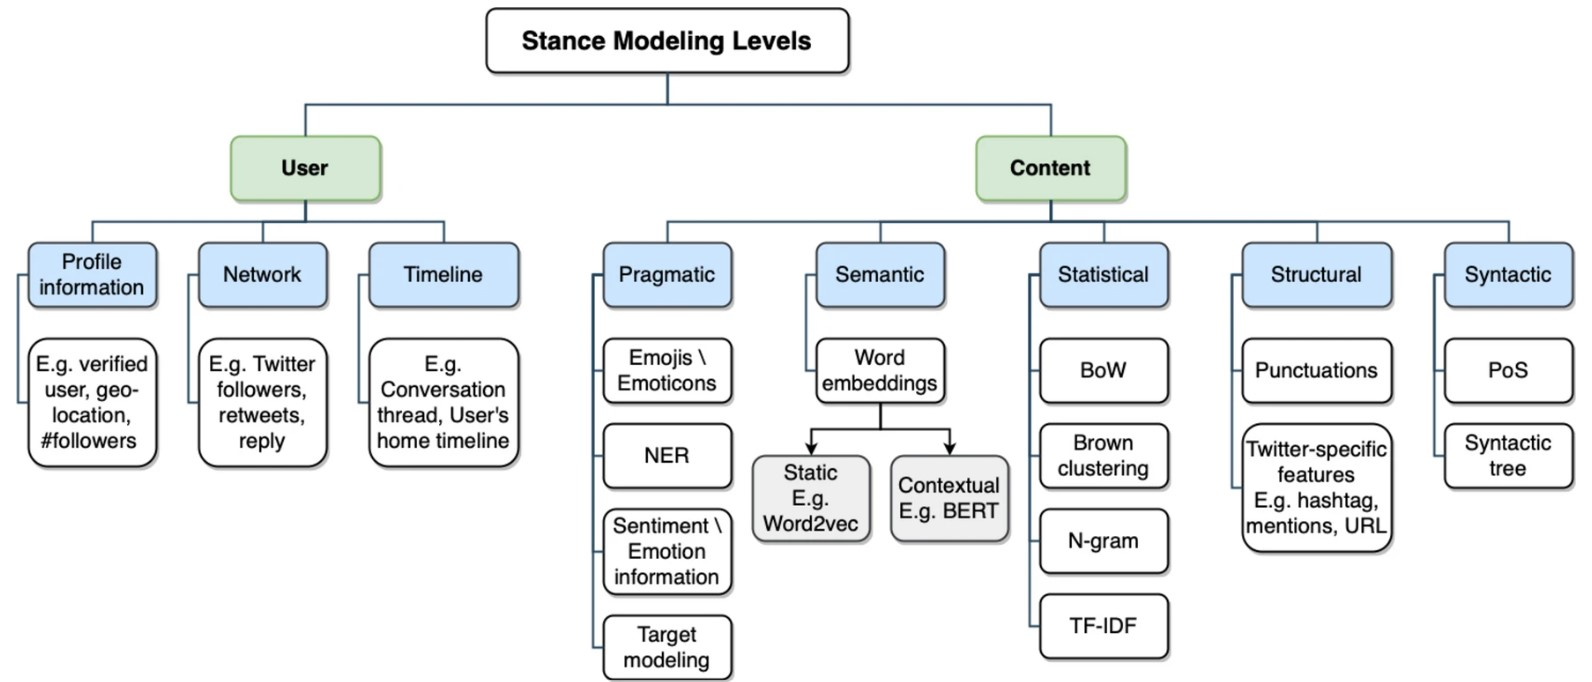
\includegraphics[width=1\linewidth]{images/stance_modeling_level.jpg}}
	\caption[مروری بر ویژگی‌های مورد استفاده در تشخیص موضع ]{مروری بر ویژگی‌های مورد استفاده در تشخیص موضع 
		\cite{Alturayeif2023} \label{stance_modeling_level}}
	
\end{figure}

\subsection[رویکردهای یادگیری ماشین مبتنی بر ویژگی]{رویکردهای یادگیری ماشین مبتنی بر ویژگی
	\LTRfootnote{\lr{Feature-Based Machine Learning Approaches}}}
%\begin{enumerate}
%	\item رویکردهای یادگیری ماشین مبتنی بر ویژگی
	%\LTRfootnote{Feature-Based Machine Learning Approaches}
	
	روش
	\lr{SVM}
	متداول‌ترین رویکرد یادگیری ماشین مبتنی بر ویژگی برای تشخیص موضع می‌باشد
	\cite{10.1145/3097286.3097288, 10.1145/3132169, mohammad-etal-2016-semeval, 10.1145/3269206.3271783, Sobhani2016DetectingSI}. 
این مدل در بیش از 40 پژوهش مورد استفاده قرار گرفته است. همچنین
	\lr{Logistic Regression}\cite{Kucher2020, 10.1007/978-3-030-14687-0_16}،
	\lr{naïve Bayes}
	و درخت تصمیم جز رده‌بند‌های متداول استفاده شده هستند. از دیگر الگوریتم‌های استفاده شده می‌توان به
	\lr{KNN}
	و 
	\lr{k-means	clustring}\cite{10.1007/978-3-319-66429-3-70}
	اشاره کرد.


مارتین و همکاران
\cite{tutek-etal-2016-takelab}
ترکیبی از چندین روش یادگیری را برای حل مسئله تشخیص موضع پیشنهاد می‌کنند. در این پژوهش از چهار مدل شامل 
\lr{SVM}، 
\lr{Random Forest}، 
\lr{Gradient Boosting} و 
\lr{Logistic Regression}
استفاده می‌شود. این الگوریتم برای ترکیب نتایج به دست آمده از چهار مدل نام برده شده،از الگوریتم ژنتیک استفاده می‌کند. ویژگی‌های واژگان به عنوان ورودی مدل برای ردە بندی انتخاب می‌شوند. این ویژگی‌ها شامل بازنمایی لغات،
\lr{n-gram}
در سطح کلمه و کاراکتر می‌باشد. همچنین تعدادی ویژگی مخصوص حل مسئله تشخیص موضع نیز تعریف کردند. این ویژگی‌ها شامل تعداد هشتگ‌ها، تعداد برخی کلمات خاص و یا غلط‌های املایی می‌باشد. این ویژگی‌ها به صورت دستی تعریف می‌شوند.


	مشیل و همکاران
	\cite{wojatzki-zesch-2016-ltl}،
	روش ردە بندی پشت سر هم
	\LTRfootnote{Stacked Classifications}
	را برای حل تشخیص موضع معرفی کردند. در واقع ردە بندی سه کلاسه در دو مرحله، با حل دو ردە بندی دو کلاسه انجام می‌شود. مرحله اول مشخص می‌کند آیا موضعی وجود دارد یا خیر. خروجی این مرحله دو بر چسب بدون موضع 
	\lr{(None)}
	یا با موضع مشخص
	\lr{(Against/Favor)}
است. سپس در صورت نیاز، در مرحله دوم برچسب نهایی از بین موافق یا مخالف انتخاب می‌شود. ردە بند استفاده شده در این روش، مدل
 SVM
 می‌باشد. واژگان موضع
 \LTRfootnote{Stance-lexicon Features}
  از مهم ترین ویژگی‌هایی است که برای ردە بندی به عنوان ورودی به مدل داده می‌شود.
  \begin{figure}
  	\center{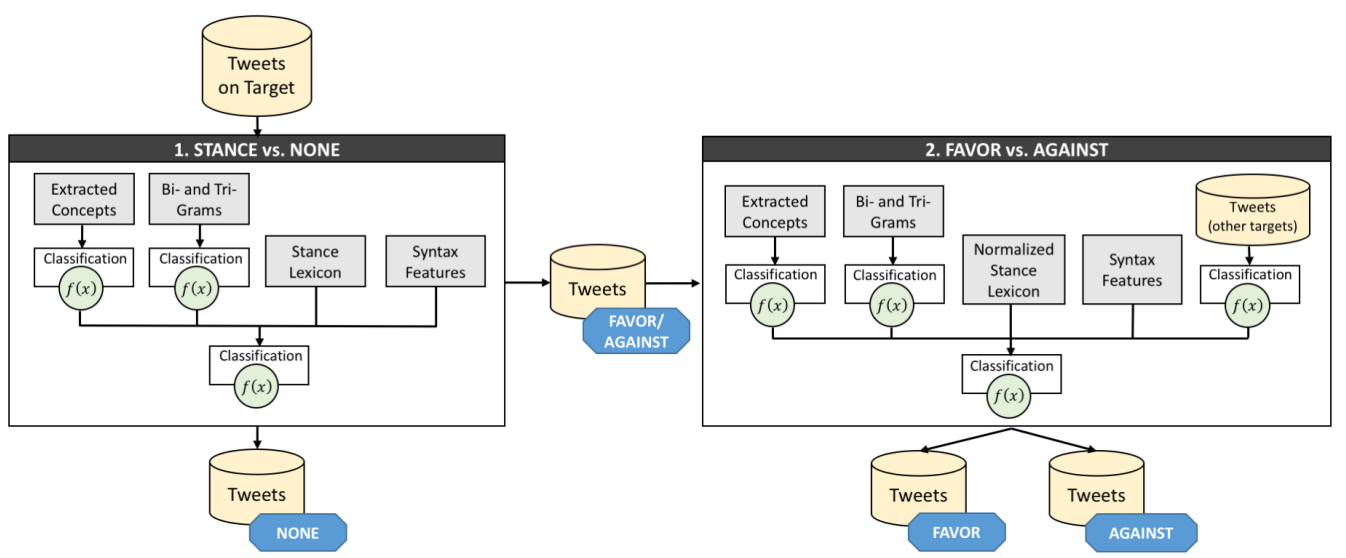
\includegraphics[width=1\linewidth]{images/StackedClassifier.PNG}}
  	\caption[معماری روش مبتنی بر 
  	\lr{Classifier Stacked}]{معماری روش مبتنی بر 
  		\lr{Classifier Stacked}
  		\cite{wojatzki-zesch-2016-ltl} \label{StackedClassifier}}
  	
  \end{figure}

\begin{table}[ht]
	\centering
	\small
	\caption[چند نمونه از پژوهش‌های مسئله تشخیص موضع]{\label{ML-Approach} چند نمونه از پژوهش‌های مسئله تشخیص موضع}
	
	\begin{tabular}{c c  c c c}
		
		پژوهش &  ویژگی & مدل & سال & مجموعه داده
		\\
		\hline
		\lr{ARC-NLP} \cite{thapa2024stance} &  
		\lr{CE \tablefootnote{contextualized embeddings}}
		& \lr{BERTweet}
		& 2023 & \lr{ClimaConvo}\\
		\hline
		\lr{HAMiSoN-G} \cite{thapa2024stance} &  
		\lr{prompt}
		& \lr{Llama}
		& 2023 & \lr{ClimaConvo}\\
		\hline
		\lr{Baseline} \cite{shiwakoti2024analyzing} &  
		\lr{CE}
		& \lr{ClimateBert}
		& 2023 & \lr{ClimaConvo}\\
		\hline
		\hline
    	\lr{PMINFM} \cite{10.1007/978-3-030-86365-4-22} &  
          \lr{CE, N-gram}
         &
         \begin{tabular}{@{}c@{}}
         	\lr{Ensemble model} \\ 
         	\lr{(RoBERTa+BiLSTM+attention)}\\
         \end{tabular}
         & 2021 & \lr{SE16-T6}\\
		\hline
         \lr{PE-HCN} \cite{zhao2020pretrained} &  
         \lr{CE, Topic modeling}
         &
          \begin{tabular}{@{}c@{}}
         	\lr{RoBERTa,} \\ 
         	\lr{Hierarchical capsule network}\\
         \end{tabular}
         & 2020 & \lr{SE16-T6}\\
		\hline
		\lr{HAN} \cite{sun-etal-2018-stance} &  
		\begin{tabular}{@{}c@{}}
			\lr{N-gram, POS, Structural} \\ 
			\lr{Sentiment lexicons}\\
		\end{tabular}
		
		& \lr{LSTM+attention}
		& 2018 & \lr{SE16-T6}\\
		\hline
		
		\cite{10.1007/978-3-030-36802-9-70} &  
		\begin{tabular}{@{}c@{}}
			\lr{SE\tablefootnote{static embeddings}, Topic modeling,} \\ 
			\lr{Sentiment labeling}\\
		\end{tabular}	
		& \lr{Multi-Task, Attention}
		& 2019 & \lr{SE16-T6}\\
		\hline
		\lr{MITRE} \cite{zarrella-marsh-2016-mitre} &  
		\lr{SE, Hashtag prediction}
		& \lr{LSTM}
		& 2016 & \lr{SE16-T6}\\
		\hline
		\hline
		\cite{Sobhani2016DetectingSI} &  
		\begin{tabular}{@{}c@{}}
			\lr{SE, Hashtag prediction} \\ 
			\lr{N-gram,Sentiment lexicons}\\
		\end{tabular}	
		& \lr{SVM}
		& 2016 & \lr{SE16-T6}\\
		\hline
		\cite{ebrahimi-etal-2016-joint} &  
		\begin{tabular}{@{}c@{}}
			\lr{N-gram, Sentiment lexicons} \\ 
			\lr{Topic modeling}\\
		\end{tabular}	
		& \lr{Maximum entropy}
		& 2016 & \lr{SE16-T6}\\
		\hline
		\lr{pkudblab} \cite{wei-etal-2016-pkudblab} &  
		\lr{SE}
		& \lr{CNN, voting scheme}
		& 2016 & \lr{SE16-T6}\\
	
		
		\hline
		\hline
		\lr{GPT3.5} \cite{zhang2022would} &  
		\lr{prompt}
		& \lr{GPT3.5}
		& 2022 & \lr{SE16-T6}\\
		\hline
		\lr{TPDG} \cite{10.1145/3442381.3449790} &  
		\begin{tabular}{@{}c@{}@{}}
			\lr{CE, Syntactical } \\ 
			\lr{dependency, Pragmatic}\\
			\lr{dependency graph}\\
		\end{tabular}
		&
		\lr{BiLSTM, GCN, attention}
		%, WT-WT
		& 2021 & \lr{SE16-T6}\\
		\hline
		\lr{SEKT} \cite{zhang-etal-2020-enhancing-cross} &  
		\begin{tabular}{@{}c@{}}
			\lr{SE, Semantic lexicons,} \\ 
			\lr{Knowledge graph}\\
		\end{tabular}
		&
		\begin{tabular}{@{}c@{}}
			\lr{GCN, BiLSTM+knowledge} \\ 
			\lr{-aware memory unit}\\
		\end{tabular}
		& 2020 & \lr{SE16-T6}\\
		\hline
		\lr{CrossNet} \cite{xu-etal-2018-cross} &  
		\lr{SE, CE, Target modeling}
		& \lr{Attention+MLP}
		& 2018 & \lr{SE16-T6}\\
		
		\hline
		\hline
		
		
	\end{tabular}
\end{table}

\iffalse
در ادامه متداول‌ترین ویژگی‌های استفاده شده در این رویکرد معرفی می‌شود. همچنین برخی ویژگی‌های در شکل
\ref{stance_modeling_level}
قابل مشاهده است.

\begin{itemize}
	\item ویژگی‌های لغوی مانند
	\lr{BOW}،
	\lr{n-gram}
	های کلمات و کاراکتر، هشتگ‌ها، کلمات نشان‌دهنده موضع، کلمات.
    \item بازنمایی برداری کلمات از جمله
	\lr{Word2Vec}،
	\lr{GloVe}.
\end{itemize}  
\fi  

\subsection[رویکردهای یادگیری عمیق]{رویکردهای یادگیری عمیق
	\LTRfootnote{\lr{Deep Learning Approaches}}}
	%\item رویکردهای یادگیری عمیق
	%\LTRfootnote{رویکردهای یادگیری عمیق}
	
	شبکه‌های عمیق در تعداد قابل توجهی از مطالعات در تشخیص موضع استفاده شدە اند.
	 \lr{RNN}
	 	  ها و انواع توسعه یافته آن 
	 \lr{(GRU ,LSTM)}	   
و شبکە‌های عصبی پیچشی
\lr{CNN}
 ها از جمله شبکە‌های عمیق استفاده شده	هستند. از میان روش‌های مطرح شده، مدل LSTM متداول ترین رویکرد استفاده شده برای تشخیص موضع
	می‌باشد. در ادامه به بررسی و معرفی برخی رویکردهای معروف پرداخته می‌شود. 
	
	برخی از ویژگی‌های متداول مورد استفاده در روش‌های یادگیری عمیق مرتبط، بازنمایی کلمات
	\lr{Word2vec}
	و
	\lr{GloVe}
	می‌باشد.
	
	در بسیاری از مطالعات اخیر از یک مکانیزم توجه استفاده شده تا عملکرد نهایی را بهبود بخشد
	\cite{10.1007/978-3-319-68783-4-2, 8489665}.
	
	مدل
	\lr{BiCond}\LTRfootnote{Bidirectional Conditional LSTM}
	توسط ایزابل و همکاران
	\cite{augenstein-etal-2016-stance}
	برای تشخیص موضع با نظارت ضعیف معرفی شده است. این روش از دو شبکه 
	\lr{BiLSTM}
	برای حل تشخیص موضع استفاده می‌کند. این دو شبکه به نحوی به یکدیگر وابسته هستند. اولین
	\lr{BiLSTM}
	وظیفه تولید بازنمایی از موضوع را به عهده دارد. دومین
	  \lr{BiLSTM}
	  نیز بازنمایی از متن توییت تولید می‌کند. نکته مهم در معماری
	  \lr{BiCond}
این است که آخرین مقادیر وزن
\lr{BiLSTM}
که موضوع را به عنوان ورودی گرفته، مقادیر اولیه
  \lr{BiLSTM}
ای است که در ادامه متن را به عنوان ورودی می‌گیرد. این وابستگی در
جهت برعکس متن اصلی نیز برقرار است. به همین دلیل است مدل شرطی نام گرفته است. این وابستگی بین موضوع و متن توییت در معماری به وضوح در شکل
\ref{bicond}
(با خط چین قرمز) قابل مشاهده است. این معماری با توجه به وابستگی که بین موضوع و متن توییت ایجاد می‌کند، عملکرد بهتری در تشخیص موضع
با نظارت ضعیف از خود نشان داده است. همچنین نتایج خوبی در تشخیص موضع برای موضوعاتی که در زمان آموزش ندیده نیز به دست آورده است.

\begin{figure}
	\center{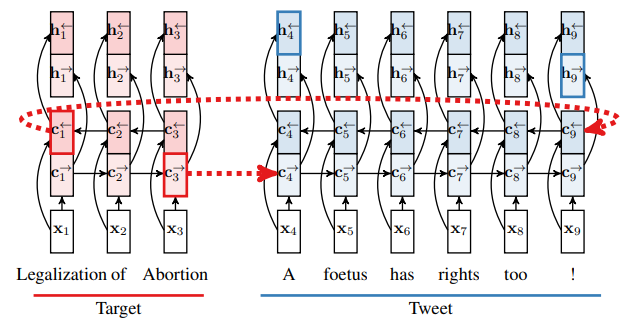
\includegraphics[width=0.8\linewidth]{images/BiCond.PNG}}
	
	\caption[معماری مدل
	\lr{BiCond}]{معماری مدل
	\lr{BiCond}\cite{augenstein-etal-2016-stance}}
	\label{bicond}
\end{figure}

مدل
\lr{PNEM}\cite{siddiqua-etal-2019-tweet}
یک روش ترکیبی برای تشخیص موضع است. در این مدل از
 \lr{CNN، LSTM}
و مکانیزم توجه استفاده شده است. ابتدا با استفاده از چندین کرنل در شبکه CNN ویژگی‌های سطح بالا از بردار متن و موضوع استخراج می‌شود. در ادامه بردار بازنمایی به دست آمده به عنوان ورودی به 
\lr{DC-BiLSTM}\LTRfootnote{Densely Connected BiLSTM}
و
\lr{NLSTMs}\LTRfootnote{Nested LSTMs}
داده می‌شود. سپس دو بردار بازنمایی تولید شده پس از عبور از مکانیزم توجه برای ردە‌بندی به شبکه کاملا متصل وارد می‌شوند. در نهایت با استفاده از بردار بازنمایی نهایی کلاس برنده مشخص می‌شود.

\begin{figure}
	\center{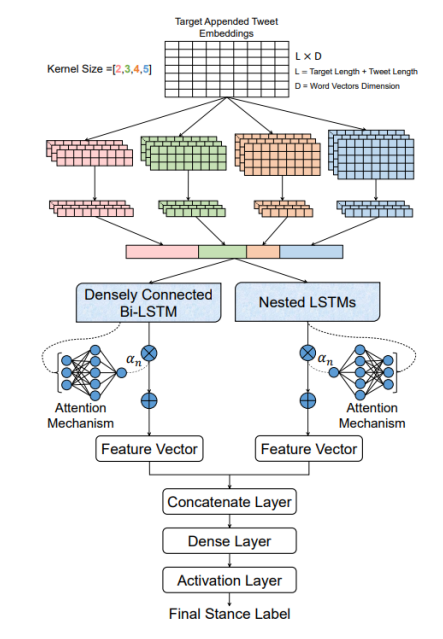
\includegraphics[width=0.4\linewidth]{images/PNEM.PNG}}
	
	\caption[معماری مدل
	\lr{PNEM}]{معماری مدل
		\lr{PNEM}\cite{siddiqua-etal-2019-tweet}}
	\label{PNEM}
\end{figure}

\subsection[مدل‌های از قبل آموزش دیده]{مدل‌های از قبل آموزش دیده}
	
	
	در سال‌های اخیر مدل‌های از پیش آموزش دیده در حوزه پردازش زبان طبیعی تعریف شده است. این مدل‌ها مبتنی بر ترنسفورمر هستند و به دلیل آموزش بر روی حجم بسیار زیادی از دادە‌ها، قابلیت بازنمایی از کلمات
دارند. 

مدل 
\lr{TweetEval}\cite{barbieri-etal-2020-tweeteval}
یک ارزیابی مبنایی 
\LTRfootnote{text}{Evaluation Benchmark}
برای شبکه اجتماعی توییتر تعریف می‌کند. 
\lr{TweetEval}
 بر روی ۷ مجموعه داده جمع آوری شده از توییتر ارزیابی شده است. بهترین نتایج با رویکرد استفاده از وزن‌های از پیش تعیین شده
\lr{RoBERTa}  
و آموزش مجدد با دادە های توییتر به دست می‌آید.

مدل
\lr{TimeLMs}\cite{loureiro-etal-2022-timelms}
 یک مدل زبانی تعریف شده بر شبکه اجتماعی توییتر است. مشابه با
\lr{TweetEval}
مدل \lr{TimeLMs} نیز از \lr{RoBERTa} استفاده می‌کند. نحوه آموزش مدل نیز مشابه با روش انتخاب شده در
\lr{TweetEval}
 است. نکته جدیدی که در این پژوهش مدل نظر قرار گرفته این است که با توجه به تغییراتی که به صورت مداوم در نحوه نگارش در شبکه‌‌های اجتماعی رخ می‌دهد، نیاز است مدل به صورت ادامه دار آموزش ببیند. این مدل بازە‌های چهار ماهه را برای این کار انتخاب کرده است. به این صورت که هر چهار ماه یه بار مدل پیشین بر روی دادە‌هایی که اخیرا از شبکه‌های اجتماعی استخراج شده آموزش ببیند. بدین ترتیب مدل زبانی همواره به روز می‌ماند.

یکی دیگر از مدل‌های زبانی استفاده شده در تشخیص موضع 
\lr{MeLT}\cite{matero-etal-2021-melt-message}
می‌باشد. روش‌های قبلی مدل زبانی را بر روی یک پیام کاربر و با حذف توکن‌های آن آموزش می‌دادند. گاهی تنها با بررسی یک پیام کاربر نمی‌توان موضع پیام نسبت به موضوع خاصی را تشخیص داد. اما زمانی که سایر متن‌های نوشته شده از کاربر بررسی می‌شود، موضع پیام قبلی که تشخیص آن سخت بود نیز میسر می‌شود. بنابراین این ایده مطرح شد که پیام‌های کاربر به صورت پشت سر هم دیده شود. به این منظور چهل پیام اخیر هر کاربر انتخاب می‌شود. و به کمک مدل زبانی از هر پیام یک بردار بازنمایی تولید می‌شود. در ادامه همان روش آموزش مدل های زبانی استفاده می‌شود. با این تفاوت که این بار به جای حذف یک توکن متن، بردار بازنمایی یک پیام کاربر
حذف می‌شود (شکل
\ref{MeLT})
و مدل زبانی آموزش می‌بیند تا این بردار را مجددا تولید کند.
\begin{figure}[H]
	\center{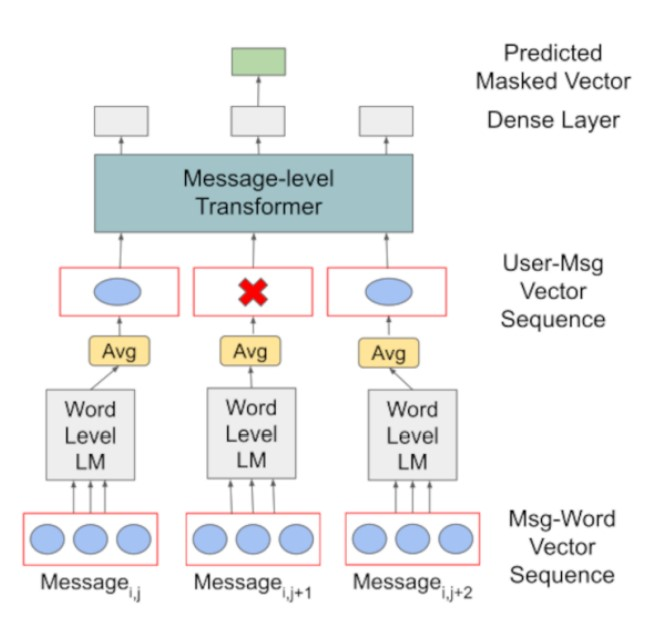
\includegraphics[width=0.6\linewidth]{images/MeLT.jpg}}
	\caption[معماری مدل
	\lr{MeLT}]{معماری مدل
		\lr{MeLT}\cite{matero-etal-2021-melt-message}}
	\label{MeLT}
\end{figure}

در پژوهش 
\cite{zhang2022would}
ژنگ و همکاران با 
\lr{ChatGPT}
و پیشنهاد پرامپت، مسئله تشخیص موضع را حل کردند. شکل
\ref{GPT_Stance}
پرامپت ارائه شده توسط این مقاله برای تعامل با 
\lr{ChatGPT}
نشان می‌دهد.
\begin{figure}[H]
	\center{
\includegraphics[width=0.8\linewidth]{images/GPT_Stance.PNG}}
	
	\caption[معماری مدل
	\lr{BiCond}]{پرامپت پیشنهادی پژوهش
		\cite{zhang2022would}}
	\label{GPT_Stance}
\end{figure}


	%\LTRfootnote{Ensemble Learning Approaches}
	
	%\item رویکرد یادگیری مجمع
	%\LTRfootnote{Ensemble Learning Approaches}
	%\item رویکرد یادگیری انتفالی
	%\LTRfootnote{Transfer Learning Approaches}
%\end{enumerate}

\iffalse


\subsection{رویکردهای مبتنی بر یادگیری با داده‌های آموزشی کم یا بدون داده آموزشی}
\lr{Zhang et al.21 employed ChatGPT for stance detection, which includes support and opposition. They used ChatGPT to classify the political stance of tweets in the SemEval-2016 and P-Stance datasets. SemEval-2016 contains 4870 English tweets, and they selected tweets with the most commonly occurring FM, LA, and HC political labels for stance classification. The P-Stance dataset has 21,574 English tweets, and they classified the stance of tweets towards Trump, Biden, and Bernie. The final results showed that on the SemEval-2016 dataset, ChatGPT achieved F1-m scores of 68.4, 58.2, and 79.5 for the FM, LA, and HC political labels, and F1-avg scores of 72.6, 59.3, and 78.0, respectively. On the P-Stance dataset, ChatGPT achieved F1-m scores of 82.8, 82.3, and 79.4 for the Trump, Biden, and Bernie political figures, and F1-avg scores of 83.2, 82.0, and 79.4, respectively.}
\fi
\section{معیار ارزیابی مسئله تشخیص موضع}
معیارهای
\lr{Precision}، 
\lr{Recall }
و 
\lr{F-Score}
معمولا در مسائل بازیابی اطلاعات
\LTRfootnote{\lr{Information Retrieval}}
و استخراج اطلاعات
\LTRfootnote{\lr{Information Extraction}}
مورد استفاده قرار می‌گیرد. معیار
\lr{F-Score}
 با وزن‌دهی بر دو معیار
 \lr{Precision}
 و
 \lr{Recall}
  محاسبه می‌شود. معیار ارزیابی
  \lr{F-Score}
همچنین در مسئله تشخیص موضع با سه کلاس نیز مورد قرار می‌گیرد. پرکاربردترین نسخه
\lr{F-Score}
 به صورت میانگین کلان
 \LTRfootnote{\lr{Macro Average}}
است که صورت زیر محاسبه می‌شود.
 \begin{equation}
	Accuracy = \frac{TP+TN}{TP+TN+FP+FN}
\end{equation}
 
\begin{equation}
 	Precision = \frac{TP}{TP+FP}
\end{equation}

\begin{equation}
	Recall = \frac{TP}{TP+FN}
\end{equation}

\begin{equation}
	F1 = \frac{2*Precision*Recall}{Precision+Recall} = \frac{2*TP}{2*TP+FP+FN}
\end{equation}



%!TeX root=main.tex

\chapter{روش پیشنهادی برای تشخیص موضع با نظارت}
\thispagestyle{empty}

تغییرات اقلیمی از جمله مهم‌ترین وقایع محیط زیستی عصر حاضر می‌باشد که بر جوامع انسانی تاثیر مستقیمی می‌گذارد. از سوی دیگر با بررسی نظرات کابران در شبکه‌های اجتماعی، می‌توان موضع کلی افراد جامعه نسبت به این موضوع را مورد ارزیابی قرار داد. با پیشرفت تکنیک‌های پردازش زبان طبیعی، امکان تشخیص موضع برای داده‌های شبکه اجتماعی فراهم شده است. برای پیشبرد تحقیقات در این حوزه، رویداد 
\lr{ClimateActivism} (بخش\ref{sec:ClimateActivismStance})
مسئله تشخیص موضع بر داده‌های شبکه‌ اجتماعی توییتر با موضوع تغییرات اقلیمی را برگزار کرد
\cite{thapa2024stance}.

در این پژوهش برای دستیابی به یک مدل هوش مصنوعی برای تشخیص موضع با نظارت، یک روش جستجو جامع به کار گرفته شد. در این جستجو، روش‌های مختلف پیش‌پردازش داده و معماری‌های متفاوت مورد بررسی قرار گرفته است. همچنین تکنیک‌‌های موثر بر مقابله با داده‌های نامتوازن
\LTRfootnote{Imbalance data}،
(مانند افزایش داده و انتخاب تابع ضرر متناسب) نیز استفاده شده است. در نهایت معماری پیشنهادی از ترکیب
\lr{BERTweet}
و شبکه‌ پیچشی
\lr{(CNN)}
و
\lr{Weighted Cross Entropy}
به عنوان تابع ضرر استفاده می‌کند. در ادامه این فصل، روش جستجو استفاده شده، فضا جستجو تعریف شده، جزییات معماری پیشنهادی، آزمایش‌های انجام شده و تحلیل نتایج به صورت مفصل بیان می‌شود.

\section{دادگان آموزشی}
برای آموزش، ارزیابی و مقایسه مدل پیشنهادی از مجموعه داده
\lr{ClimaConvo}\cite{shiwakoti2024analyzing}
استفاده شد. این مجموعه داده شامل شش مسئله مختلف از جمله تشخیص موضع، تشخیص طنز
\LTRfootnote{Humor Detection}
و تشخیص سخنان نفرت انگیز
~\LTRfootnote{Hate Speach Detection}
می‌باشد. در اینجا تنها از بخش تشخیص موضع دادگان استفاده شده است. توزیع داده‌های هر کلاس در جدول
\ref{dataset-statistics}
نشان داده شده است. بخش 
\ref{sec:datasetClimaConvo}
شامل توضیحات تکمیلی درباره مجموعه داده می‌باشد. شکل
\ref{token-len-distribution}
توزیع تعداد تک واژهای مجموعه داده 
\lr{ClimaConvo}
را نشان می‌دهد.
\begin{table}[ht]
	\centering
	\small
	\caption{\label{dataset-statistics} توزیع کلاس‌ها در بخش‌های آموزش، توسعه و ارزیابی مجموعه داده
	\lr{ClimaConvo}}
	
	\vspace{0.2cm}
	\begin{tabular}{ c|c|   c c c}
		\hline
		& \% & موافق & بدون نظر &  مخالف\\
		\hline
		\hline
		آموزش (\lr{Train}) & 70\% & 4328 & 2256 & 700 \\
		توسعه (\lr{Dev}) & 15\% & 897 & 511 & 153  \\  
		ارزیابی (\lr{Test}) & 15\% & 921 & 500 & 141\\
		\hline
		\hline
		مجموع & 100\% & 6146 & 3276  & 994 \\
		\hline
	\end{tabular}
\end{table}


\begin{figure}[H]
	\center{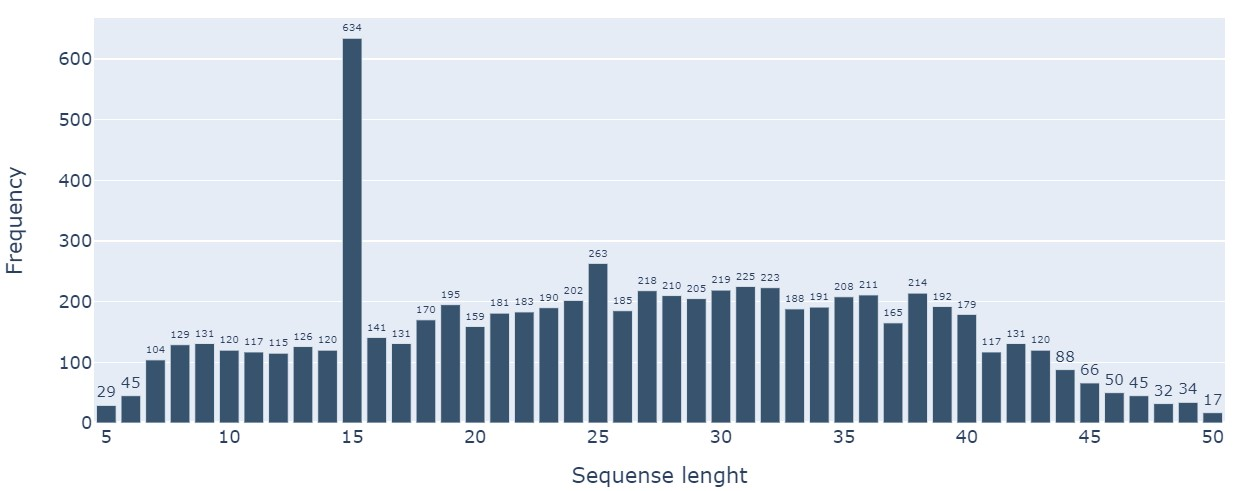
\includegraphics[width=1\linewidth]{images/tolen_len_distribution.jpg}}
	\vspace{-1cm}
	\caption{توزیع تعداد تک واژهای مجموعه داده
	\lr{ClimaConvo} \label{token-len-distribution}}
	
\end{figure}

همچنین در قسمت پایانی این فصل برای ارزیابی عملکرد مدل بر مجموعه داده‌ای که بر روی آن آموزش ندیده، دو بخش "قانونی شدن سقط جنین" و "تغییرات اقلیمی" از مجموعه داده 
\lr{SemEval}\cite{mohammad-etal-2016-semeval}
مورد استفاده قرار گرفت. جدول
\ref{dataset-statistics-semeval}
توزیع کلاس‌های مجموعه داده به ازای هر موضوع را نشان می‌دهد.
\begin{table}[ht]
	\centering
	\small
	\caption{\label{dataset-statistics-semeval} توزیع کلاس‌ها در بخش‌های ارزیابی مجموعه داده
		\lr{SemEval}}
	
	\vspace{0.2cm}
	\begin{tabular}{ c|   c c c}
		\hline
		 موضوع & موافق & بدون نظر &  مخالف\\
		\hline
		\hline
		تغییرات اقلیمی (\lr{CC}) &  11 & 35 & 123 \\
		قانونی شدن سقط جنین (\lr{LA}) &  186 & 45 & 46 \\
		\hline
		\hline
	
	\end{tabular}
\end{table}
\section{روش حل مسئله}
رویکرد ارائه شده، از روش جستجو معماری شبکه عصبی الگو می‌گیرد. بدین منظور معماری شبکه  به چهار بخش اصلی تقسیم شد. به ازای هر یک از بخش‌ها با توجه به دانش قبلی، فضای جستجو متناسب معرفی شد. در ادامه از جستجو تطبیقی برای یافتن بهترین پارامترهای مدل و ابرپارامترها استفاده شد. روش جستجو استفاده شده در مقایسه با جستجو تصادفی و جستجو شبکه‌ای مزایای زیادی دارد. این روش از پیشینه جستجو برای انتخاب پارامترهای بعدی استفاده می‌کند. همچنین در صورت ناموفق بودن یک جستجو، به صورت زودهنگام جستجو را متوقف می‌کند. بنابراین در زمان مناسب می‌تواند جستجو نسبتا جامعی انجام دهد.

از سوی دیگر داده‌های ورودی مدل نیز اهمیت ویژه‌ای دارند. از این رو هفت سطح از پیش‌پردازش داده معرفی شد تا تاثیر آن بر نتایج نهایی مورد بررسی قرار بگیرد. همچنین با توجه به نامتوازن بودن داده‌های آموزشی از  روش‌های افزایش داده برا غلبه به این مشکل استفاده شد.
در ادامه توضیحات مربوط به سطوح پیش‌پردازش داده، روش افزایش داده و رویکرد جستجو معماری به صورت مفصل بیان می‌شود.

\subsection{پیش‌پردازش داده‌ها}\label{sec:preprocess}
آماده‌سازی داده‌های مناسب و با کیفیت یکی از مهم‌ترین بخش‌های آموزش یک مدل یادگیری عمیق است.
ابتدایی‌ترین گام در مسائل پردازش زبان طبیعی، پیش‌پردازش دادە‌ها است که به ارتقاء کیفیت دادە‌ها و استخراج معنای بهتر از آن‌ها کمک می‌کند. پیش‌پردازش دادە‌ها به معنای تمیز کردن و سازماندهی دادە‌های خام به شکل قابل فهم برای آموزش مدل‌های یادگیری عمیق است.

 داده‌های متنی شبکه‌های اجتماعی (همانند توییتر) معمولا شامل نویز و عباراتی هستند که ممکن است مدل را دچار خطا کند. در فرآیند پیش‌پردازش داده‌، رویکرد اصلی این است که هیچ داده‌‌ای دور ریخته نشود و حداکثر اطلاعات از داده‌های متنی موجود استخراج شود. اما به دلیل محدودیت در داده‌های آموزشی، وجود نویز در داده‌ها ممکن است آموزش مدل را با مشکل روبرو کند. در ادامه هفت سطح متفاوت برای پیش‌پردازش داده معرفی می‌شود. روش‌های معرفی شده به صورت سلسله مراتبی هستند. بدین معنا که هر روش نسبت به روش قبلی، اطلاعات بیشتری را حذف می‌کند یا تغییر می‌دهد.
 
\begin{enumerate}
	\item 	\textbf{نگهداشت داده‌های اصلی}:
در این رویکرد فرض کردیم بهترین روش عدم تغییر داده‌های اصلی می‌باشد. در این روش متن داده‌های موجود بدون هیچ تغییری به عنوان ورودی مدل در نظر گرفته می‌شود.
	\item \textbf{ حذف آدرس‌ اینترنتی}
	\LTRfootnote{\lr{URL}}
	: با توجه به اینکه اغلب آدرس‌های اینترنتی به صورت مختصر وجود داشتند (به عنوان مثال
	\href{https://t.co/rs1vhBp2ax}{\lr{https://t.co/rs1vhBp2ax}})
	امکان یافتن الگو از آن‌ها ممکن نبود. بنابراین در این رویکرد فقط آدرس اینترنتی حذف شده و مابقی متن را تغییری نکرد.
	\item حذف نام‌کاربری
	\LTRfootnote{\lr{Username}}:
فرض ما این است وجود نام‌کاربری بدون اینکه اطلاعات دیگری از کاربران داشته باشیم بیشتر موجب گمراهی مدل می‌شود. برای بررسی صحت فرض مطرح شده، این رویکرد را نیز در آزمایش‌های خود قرار دادیم.
	\item حذف همزمان نام کاربری و آدرس اینترنتی:
رویکرد دوم و سوم را برای بررسی اثربخشی همزمان آن‌ها با هم اعمال شد.

	\item حذف همزمان نام کاربری و آدرس اینترنتی و جدا کردن هشتگ: 
	در شبکه‌های اجتماعی همچون توییتر برای بیشتر دیده شدن توییت‌ها و همراهی با رویدادی خاص، گاها هشتگ‌هایی در متن اصلی توییت استفاده می‌شود. استفاده از  هشتگ‌ها جستجو آن‌ها را نیز ساده‌تر می‌کند. در این رویکرد برای تمیز کردن داده‌ها هشتگ‌ها به صورت یک عبارت در آوردیم به گونه‌ای که
 \lr{\texttt{\#FridaysForFuture} }
به
 \lr{\texttt{Fridays For Future}}
 تبدیل می‌شود. انتطار می‌رود بعد از جداسازی هشتگ‌ها عبارت قابل فهم‌تری داشته باشیم.
 
	\item حذف همزمان نام کاربری و آدرس اینترنتی و جدا کردن هشتگ و کوچک کردن حروف:
در زبان انگلیسی معمولا کلمات در ابتدا جمله با حروف بزرگ شروع می‌شوند. از طرفی گاهی کلیه حروف یک کلمه بنا به دلایلی خاص از جمله تاکید، خشم یا عصبانیت به صورت بزرگ نوشته می‌شود. از سوی دیگر دو کلمه
\lr{Book}
و
\lr{book}
هم معنی هستند اما با توجه به اختلاف در حروف اول دو بازنمایی متفاوت در مدل‌های هوش مصنوعی پیدا می‌کنند. یکی از گام‌های پیش‌پردازش داده‌ها کوچک کردن همه حروف
\LTRfootnote{Lower Casing}
می‌باشد. در این سطح از پیش‌پردازش داده قصد داریم تاثیر این عمل بر نتیجه نهایی  مدل را به دست بیاوریم.
	\item تمیز کردن کامل داده‌ها:
	این سطح شامل کامل‌ترین پیش‌پردازش می‌باشد و علاوه بر همه موارد رویکرد ششم، کلمه‌های توقف
	\LTRfootnote{\lr{Stop Words}}
	و علائم دستوری نیز حذف می‌شوند.
\end{enumerate}

در بخش
~\ref{sec:data-cleaning-impact}،
 عملکرد هر یک از روش‌های پیش‌پردازش مورد بررسی قرار می‌گیرد.

\subsection{افزایش داده}\label{sec:dataaug}
یکی از روش‌های استفاده شده برای غلبه بر مشکلات ناشی از مجموعه داده کوچک و نامتوازن، استفاده از تکنیک‌های افزایش داده می‌باشد. در این پژوهش برای افزایش داده، از مدل مبتنی بر
\lr{T5}
که بر روی مجموعه داده‌
\lr{ChatGPT paraphrase}\cite{chatgpt-paraphrases-dataset}
آموزش دیده
\cite{chatgpt-paraphraser}
، برای افزایش داده استفاده می‌کنیم. این مدل آموزش دیده تا متن ورودی را به گونه‌ای دیگر بازنویسی
\LTRfootnote{Paraphrase}
 کند. برای افزایش داده به کمک این روش، توییت‌هایی کلاس مخالف را به عنوان ورودی مدل دادیم. مدل به ازای هر متن، 5 بازنویسی از آن را تولید کرده است. توزیع مجموعه داده آموزشی بعد از افزایش داده در شکل~
 \ref{dataset-distribution}
 قابل مشاهده است. در بخش
 ~\ref{sec:data-aug-impact}،
تاثیر افزایش داده بر نتایج به دست آمده مورد بررسی قرار می‌گیرد.

\begin{figure}[H]
	\center{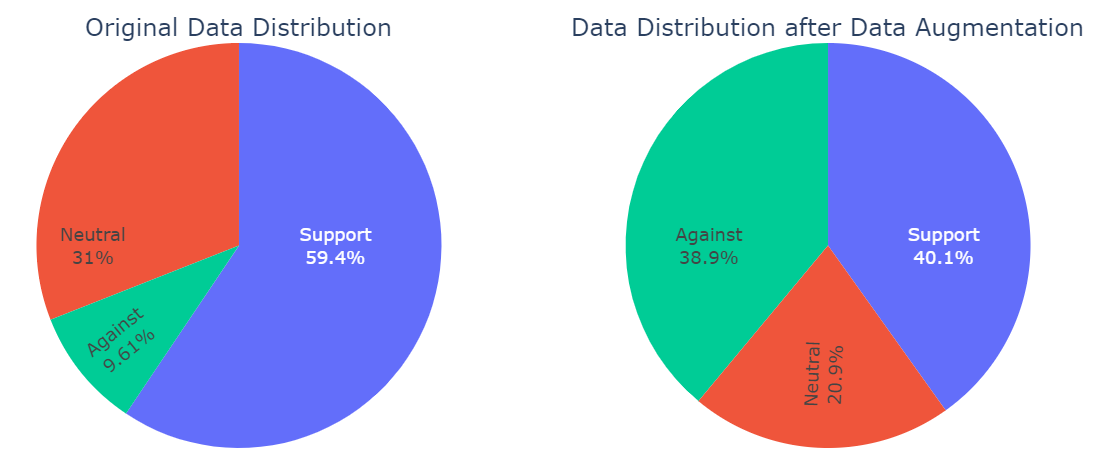
\includegraphics[width=0.8\linewidth]{images/dataset_distribution.png}}
	\caption{توزیع کلاس‌ها قبل و بعد از افزایش داده.}
	\label{dataset-distribution}
\end{figure}
\subsection{جستجو معماری}

در این پژوهش، یک روش جستجو قاعده‌مند
\LTRfootnote{\lr{Systematic}}
 برای یافتن بهترین معماری مدل استفاده شده است. برای تعریف فضا جستجو، ابتدا معماری پیشنهادی به چهار بخش اصلی تقسیم شد. سپس برای هر یک از چهار بخش اصلی فضای جستجو مناسب تعریف شد. برای تعیین مناسب‌ترین پارامترها برای هر بخش، آزمایش‌های متعددی با پیکربندی‌های مختلف انجام داده شد و مقادیر بهینه در فضای جستجوی تعریف‌شده جستجو شد (جدول\ref{Architecture-search-space}). جستجو در فضای تعریف شده با استفاده از کتابخانه
\lr{Optuna} 
، که از نمونه‌بردار با استفاده از الگوریتم 
\lr{TPE (Tree-structured Parzen Estimator) }
استفاده می‌کند، انجام شد. پیکربندی مدل بهینه را بر اساس امتیاز
\lr{Macro-F1} 
در مجموعه توسعه 
\LTRfootnote{Development Set}
انتخاب شد. فضا جستجو تعریف شده برای هر بخش در جدول 
\ref{Architecture-search-space}
قابل مشاهده است.
\begin{table}[h!]
	\centering
	\caption{\label{Architecture-search-space}فضای جستجو معماری پیشنهادی}
	\vspace{0.2cm}
	\begin{tabular}{c  |c }
		\hline
		پارامتر & فضا جستجو\\
		\hline
		بازنمایی کلمات&
		\lr{[BERT, RoBERTa, BERTweet, XLM-RoBERTa, DEBERTA]}\\
		رده‌بند &
		\lr{[FNN, CNN]}
		\\
		\lr{N\_last\_layer} & $[1, 2, 3, 4, 5]$\\
		بهینه‌ساز &
		\lr{[Adam, AdamW, RMSprop, SGD]}
		\\
		تابع ضرر &
		\lr{[Weighted  Cross Entropy, Focal]}
		\\      
		
		
		\hline
		\hline
	\end{tabular}
\end{table}

\begin{enumerate}
	\item بازنمایی کلمات
	\LTRfootnote{Embedding}: برای این بخش تعدادی از مدل‌های کدگذار
\LTRfootnote{Encoder-Only}
که نتایج بهتری در مسائل مشابه کسب کردند را انتخاب کردیم. استفاده از این مدل‌ها در مسائل رده‌بندی
\LTRfootnote{Classification Task}
، متداول‌تر از مدل‌های کدگشا‍~
\LTRfootnote{Decoder-only}
و کدگذار-کدگشا~
\LTRfootnote{Encoder-Decoder}
هستند (جدول~\ref{Architecture-search-space}). 
	\item رده‌بند
	\LTRfootnote{Classifier}:
	در این بخش دو معماری متفاوت را بررسی کردیم.
	\begin{itemize}
		\item معماری شبکه عصبی تماما متصل (FNN)
		\LTRfootnote{Fully Connected Neural Networks}
		
در این بخش	ما از یک معماری سه لایه خطی، به همراه تابع فعال‌سازی 
		\lr{ReLU}و
		\lr{dropout} 
		استفاده ‌می‌کنیم. در نهایت
		\lr{Softmax}
		را بر روی خروجی اعمال می‌کنیم.
				
		\item معماری شبکه عصبی پیچشی (CNN)
		\LTRfootnote{Convolutional Neural Networks}
		
		ایده اصلی معماری استفاده شده مشابه کار سفایا و همکاران
\cite{safaya-etal-2020-kuisail}
		می‌باشد. تفاوت اصلی در این است که به جای 4 لایه آخر، فضا جستجو برای تعداد لایه‌ها تعریف کرده و با آزمایش مقادیر مختلف، بهترین مقدار را به دست می‌آوریم. در این معماری 
		\lr{Embedding} 
		به تعداد 32 فیلتر کانولوشنال موازی با اندازه متفاوت وارد می‌شود (768‍×1، 786×2، 786×3، 786×4، 786×5). معماری پیشنهاد شده مشابه شبکه
		\lr{Inception}
		در بینایی ماشین می‌باشد. بعد از اعمال فیلتر کانولوشنال، تابع فعال‌سازی
		\lr{ReLU}
و 
\lr{Global Max-Pooling}
بر خروجی مرحله قبل اعمال می‌شود. خروجی تولید شده بعد از 
\lr{Faltten}
شدن به یکدیگر
\lr{Concate}
می‌شوند. در انتها با اعمال 
\lr{Softmax}
خروجی نهایی حاصل می‌شود. شکل~\cite{safaya-etal-2020-kuisail} 
معماری رده‌بند متشکل از شبکه عصبی پیچشی را نشان می‌دهد.
		
		
\begin{figure}[H]
	\center{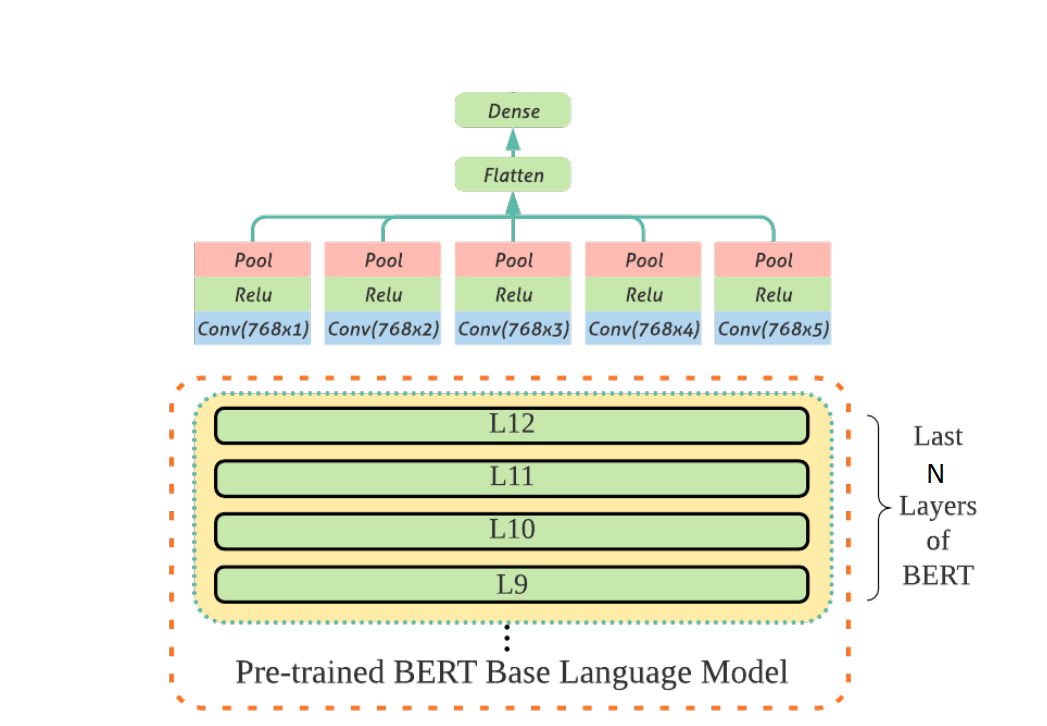
\includegraphics[width=0.7\linewidth]{images/BERT-CNN.PNG}}
	\caption[رده‌بند با شبکه عصبی پیچشی]{رده‌بند با شبکه عصبی پیچشی
\cite{safaya-etal-2020-kuisail}	\label{Bert_CNN}}
\end{figure}
		
	\end{itemize}
	\item بهینه‌ساز
	\LTRfootnote{Optimizer}: فضای جستجو تعریف شده برای بهینه‌سازها شامل چهار بهینه‌ساز معروف، که عملکرد مثبتی از خود نشان دادند، می‌باشد (جدول~\ref{Architecture-search-space}).
	\item تابع ضرر
	\LTRfootnote{Loss Function}:
از‌ آنجایی که با داده‌های نامتوازن و مسئله رده‌بندی مواجه هستیم دو تابع ضرر متفاوت با توجه به شرایط تعریف کردیم.
	
	\begin{itemize}
		\item تابع ضرر
		\lr{Focal}:
		تابع ضرر
		\lr{Focal} \cite{Lin-2017-ICCV}
		با کاهش وزن داده‌های کلاس اکثریت (که به آسانی توسط مدل یادگرفته می‌شوند) در زمان آموزش مدل، تاثیر نامتوازن بودن داده را کم می‌کند. این تابع ضرر به یادگیری صحیح داده‌های سخت‌تر (کلاس اقلیت) تاکید بیشتری دارد تا به این صورت عملکرد نهایی بهبود پیدا کند.
		
		\item تابع ضرر
		\lr{Weighted Cross Entropy}:
		این تابع ضرر گونه‌ای از تابع ضرر استاندارد
		\lr{Cross Entropy}
		می‌باشد به گونه‌ای که به کلاس‌های مختلف، وزن‌های متفاوتی اختصاص می‌دهد. وزن‌های هر کلاس با محاسبه نسبت معکوس تعداد داده‌های آموزشی هر کلاس به کل داده‌های آموزشی به دست می‌آید. به عبارت دیگر اشتباهات کلاس‌ اقلیت نیز اهمیت پیدا می‌کند.
	\end{itemize}
\end{enumerate}

\subsection{انتخاب ابرپارامترها}

انتخاب دقیق ابرپارامترهای استفاده شده در زمان آموزش مدل، از اهمیت ویژه‌ای برخوردار است. در این قسمت از کتابخانه
\lr{Optuna} 
و نمونه‌بردار
\lr{TPE (Tree-structured Parzen Estimator) }
استفاده شد. در این شیوه جستجو ابرپارمترها در هر آزمایش، پارامترها در فضا جستجو انتخاب می‌شوند. این الگوریتم معیاری را برای مقایسه نتیجه آزمایش‌های انجام شده در نظر می‌گیرد. در این پژوهش معیار
\lr{F1-Score}
به عنوان معیار اصلی تعریف شد. در نهایت ترکیبی از فراپارامترها که باعث افزایش معیار 
\lr{F1-Score}
شوند به عنوان پیشنهاد نهایی ارائه می‌شود. همچنین الگوریتم قابلیت خاتمه زودهنگام آزمایش‌هایی با نتایج نامناسب را دارد. جدول
\ref{hyperparam-search-space}
فضای جستجو ابرپارمترهای مدل را نشان می‌دهد.
\begin{table}[h!]
	\centering
	\caption{\label{hyperparam-search-space}فضا جستجو ابرپارامترها}
	\vspace{0.2cm}
	\begin{tabular}{c  |c }
		\hline
		ابرپارامتر & فضای جستجو\\
		\hline
		\lr{Dropout}  &  $[0.1 :  0.5]$\\
		نرخ یادگیری & $[1e^{-5} :  1e^{-2}]$\\
		تعداد دوره
		(\lr{Epoch})&
		$[4, 8]$\\
		اندازه دسته (\lr{Batch Size}) & $[4, 8]$\\
		پارامتر گاما تابع ضرر
		\lr{Focal} & $[1, 2, 3, 4, 5]$\\
		\hline
		\hline
	\end{tabular}
	\centering
\end{table}




\section{آزمایش‌ها و تحلیل نتایج}
برای یافتن بهترین معماری و تحلیل اثرگذاری بخش‌های مختلف بر نتیجه اصلی اقداماتی صورت گرفته است. در این بخش به توضیح اقدامات انجام شده پرداخته می‌شود.

\subsection{گام اول : تحلیل نحوه عملکرد الگوریتم جستجو}

	برای شناخت بیشتر از عملکرد ابزار
	\lr{optuna}
دو آزمایش طراحی و اجرا شد. هدف از انجام این آزمایش‌ها بررسی میزان تکرارپذیری و قابل اتکا بودن این ابزار بود. 
\begin{enumerate}
	\item
	 جستجو در فصای نمونه تعریف شده به ازای هر کدام از روش‌های تمیز کردن داده‌ها 3 بار و هر کدام به تعداد 10 ترایال
	 \footnote{منظور از ترایال همان
	 \lr{trial}
 می‌باشد. آزمایشی که در آن یک بار از فضای جستجو مقادیر پارامترها انتخاب شده و عملکرد مدل بر اساس آن مقادیر مورد بررسی قرار می‌گیرد. در این گزارش برای نزدیک بودن متن نوشته به توضیحات مربوط به 
\lr{optuna}
از همان اصطلاح ترایال استفاده شده است.}
	  تکرار شد (یعنی 10 بار پارامترهای مختلف در فضا جستجو انتخاب شد و مدل آموزش داده شد).  هدف از این بخش بررسی بهترین پارامترهایی است که بعد از 10 بار جستجو  به دست می‌آید. آیا همواره به پارامترهای یکسانی می‌رسد؟
	
	\item
	
	جستجو در فضای نمونه به تعداد ترایال‌های مختلف (10، 20، 40) تکرار شد تا تاثیر افزایش تعداد ترایال بر عملکرد نهایی مدل را به دست بیاید (با مقایسه	
	\lr{F1-Score}).
	
\end{enumerate}

برای جستجو به تعداد ده ترایال، نتایج به دست آمده نشان می‌دهد بهترین پارامترهای پیشنهادی هر کدام از جستجوها تا حدودی با یکدیگر متفاوت بودند. اما 
\lr{F1-Score}
نهایی بهترین مدل تقریبا یکسان بودند. از طرفی با افزایش تعداد ترایال‌ها به 20، نتیجه نهایی بهبود داشت و پارامترهای دقیق‌تری انتخاب شدند. منتها نتایج 40 ترایال و 20 ترایال اختلاف معناداری با یکدیگر نداشتد.

با توجه به نتایج به دست آمده تصمیم گرفته شد آزمایش‌ها را به تعداد 20 ترایال تکرار کرده و بهترین پیکربندی به دست آمده، به عنوان مدل پیشنهادی ارائه شود.

\subsection{گام دوم : به دست آوردن پارامترهای مدل با عملکرد مطلوب  }
در بخش~
\ref{sec:preprocess}
هفت سطح مختلف برای پیش‌پردازش داده‌ها معرفی شد. همچنین در بخش~ 
\ref{sec:dataaug}
نحوه افزایش داده به تفصیل توضیح داده شد. آزمایش‌ها در دو حالت با افزایش داده و بدون افزایش داده تکرار شدند. بنابراین چهارده پیکربندی مختلف تعریف شد. به ازای هر پیکربندی، 20 بار در ترایال‌های مختلف با استفاده از الگوریتم جستجو
\lr{Optuna}
، پارامترهای متفاوتی انتخاب شد و سپس مدل با آن پارامترها آموزش داده شد. همچنین مکانیزمی برای توقف ترایال‌هایی که نتایج آن‌ها در جهت بهبود پیش نمی‌رود نیز وجود دارد. همان‌طور که در بخش‌های قبل اشاره شد، به دلیل بزرگ بودن فضا جستجو، جستجو شبکه‌ای بسیار زمان‌بر و عملا غیر ممکن خواهد بود. برای اینکه بتوان فضای جستجو نسبتا وسیع‌تری را مورد بررسی قرار داد از جستجو تطابقی، که پیشینه جستجو را در انتخاب‌های بعدی در نظر می‌گیرد، استفاده شد. بنابراین در این آزمایش‌ها همه ترکیب‌های ممکن بررسی نشده است اما الگوریتم جستجو به صورت هوشمند در هر ترایال بهترین پارامترها را انتخاب می‌کند و در صورت لزوم ادامه آموزش یک ترایال را متوقف می‌کند. چنین فرآیندی سرعت رسیدن به پارامترهای بهینه را افزایش می‌دهد.
\begin{table*}[h!]
	\centering
	\scriptsize
	\caption[نتایج به دست آمده بر روی مجموعه داده
	\lr{ClimateCanvo Stance} بخش ارزیابی. ]{\label{result}
		نتایج به دست آمده بر روی مجموعه داده
		\lr{ClimateCanvo Stance}
		بخش ارزیابی. روش‌های پیش‌پردازش داده:(
		\lr{C1}: نگهداشت داده‌های اصلی, 
		\lr{C2}: حذف آدرس‌ اینترنتی, 
		\lr{C3}: حذف نام‌کاربری, 
		\lr{C4}: حذف نام کاربری و آدرس اینترنتی به صورت همزمان,     
		\lr{C5}: حذف نام کاربری و حذف آدرس‌ اینترنتی به صورت همزمان و جدا کردن هشتک, 
		\lr{C6}: حذف نام کاربری و آدرس‌ اینترنتی به صورت همزمان و جدا کردن هشتک و کوچک کردن حروف,
		\lr{C7}: تمیز کردن کامل داده‌ها).}
	\vspace{0.2cm}
	\begin{tabular}{c  |c |c c  c  c|c c  c  c}
		\hline
		پیش‌پردازش & افزایش داده &  کدگذار&رده‌بند & تابع ضرر & بهینه‌ساز &
		\lr{F1-Score} & \lr{Recall} & \lr{Precision}& \lr{Accuracy}\\
		\hline
		%report_climate_stance_experiment_on_column_tweet_trial_2
		% , D=0.5 0.68822023
		
		
		\lr{C1} & - &\lr{RoBERTa}&  \lr{CNN(N=1)}& \lr{WCE} & \lr{SGD} &  $71.74$ & $69.94$ & $74.83$& $68.82$\\
		% \tablespace
		\hline
		\hline
		% \tablespace
		%report_climate_stance_experiment_on_column_tweet_remove_url_trial_13 ACC = 0.6491
		% , D=0.2
		\lr{C2} & - & \lr{XLM-RoBERTa}  & \lr{CNN(N=3)}& \lr{WCE} & \lr{AdamW} &  $69.80$ & $69.38$ & $74.16$& $64.91$\\ 
		%report_climate_stance_experiment_on_column_tweet_remove_url_trial_19
		% , D=0.4
		\lr{C2} & - & \lr{BERT}& \lr{CNN(N=2)}& \lr{WCE} & \lr{SGD} &  $70.28$ & $68.64$ & $73.82$ & $66.00$\\
		%report_climate_stance_experiment_on_column_tweet_remove_username_trial_3
		%        0.73815621	0.71894142	0.688951494	0.795527692
		% (D=0.4)
		
		% report_climate_stance_experiment_on_column_data_aug_tweet_remove_url_trial_0
		% 0.701664533	0.687506824	0.662705354	0.752605222
		\lr{C2} & + & \lr{BERT}& \lr{CNN(N=3)} &  \lr{WCE}& \lr{SGD} & $68.75$ & $66.27$ & $75.26$& $70.16$\\
		
		\hline
		\hline
		\lr{C3} & - & \lr{RoBERTa}&  \lr{FNN} & \lr{WCE} & \lr{SGD} & $71.89$ & $68.89$ & $79.55$& $73.81$\\
		
		%report_climate_stance_experiment_on_column_data_aug_tweet_remove_username_trial_4
		\lr{C3} & + & \lr{XLM-RoBERTa} &  \lr{CNN(N=3)} & \lr{F(g=4)} & \lr{SGD} & $68.59$ & $68.51$ & $75.93$& $69.84$\\
		\hline
		\hline
		%report_climate_stance_experiment_on_column_tweet_remove_url_username_trial_0
		% 0.695262484	0.71827397	0.695655047	0.748081657
		% - & - &  - & - &  - & - & -\\
		% , D=0.4
		\lr{C4} & - & \lr{XLM-RoBERTa}  &\lr{CNN(N=2)}&  \lr{WCE} & \lr{RMSprop}&  $71.82$ & $69.56$ & $74.80$ & $69.52$\\
		%trial_2
		%0.728553137	0.723104075	0.696190696	0.769851624
		% , D=0.5
		\lr{C4} & - & \lr{BERT} & \lr{CNN(N=5)} &  \lr{WCE} & \lr{SGD} &  $72.82$ & $69.56$ & $74.80$ & $72.85$\\
		%trial_4
		%0.725992318	0.739746891	0.70919688	0.781799265
		% , D=0.2
		\lr{C4}& - & \lr{XLM-RoBERTa} & \lr{CNN(N=3)} &  \lr{F(g=1)} & \lr{SGD} &  $73.97$ & $70.91$ & $78.17$ & $72.59$\\
		%trial_12
		%0.710627401	0.715227463	0.683140419	0.766553658
		%(D=0.5)
		\lr{C4}& - & \lr{RoBERTa}& \lr{FNN} &  \lr{WCE} & \lr{RMSprop} &  $71.52$ & $68.31$ & $78.17$ & $70.06$\\
		%trial_15
		%0.731754161	0.727294616	0.693864994	0.788514218
		%, D=0.3
		\lr{C4}& - & \lr{XLM-RoBERTa} & \lr{CNN(N=4)} &  \lr{WCE}& \lr{SGD} &  $72.72$ & $69.38$ & $78.85$ & $73.17$\\
		%report_climate_stance_experiment_on_column_data_aug_tweet_remove_url_username_trial_0
		%0.741357234	0.748312045	0.71640203	0.794630353
		
		% C4& \Checkmark &  BERTweet&CNN(\textbf{N=5}) &  \textbf{WCE}&\textbf{SGD} &  \textbf{74.83} &\textbf{ 71.64} &\textbf{ 79.46}&\textbf{74.13}\\
		
		
		\textbf{\lr{C4}}& \textbf{+} &  \textbf{\lr{BERTweet}} & \textbf{\lr{CNN(N=5)}} &  \textbf{\lr{WCE}} & \textbf{\lr{SGD}} & \textbf{\lr{74.47}} & \textbf{\lr{70.31}} & \textbf{\lr{79.31}}& \textbf{\lr{73.11}}\\
		%report_climate_stance_experiment_on_column_data_aug_tweet_remove_url_username_trial_2
		%0.701664533	0.706468713	0.675635533	0.756350482
		
		\lr{C4}& + & \lr{BERT} & \lr{CNN(N=4)} &  \lr{WCE} & \lr{SGD} &  $70.64$ & $67.75$ & $75.63$& $70.01$\\
		
		\hline
		\hline
		% report_climate_stance_experiment_on_column_tweet_remove_url_username_splite_hasghtag_trial_2
		%trial_2
		%0.677336748	0.713373105	0.687480629	0.754339459
		% (D=0.1)
		\lr{C5} & -& \lr{DEBERTA} &  \lr{FNN} & \lr{WCE} & \lr{Adam} &  $71.33$ & $68.78$ & $75.43$ & $67.73$\\
		%trial_5
		%0.721510883	0.727001956	0.6963022	0.771830242
		% , D=0.2
		\lr{C5} & - & \lr{XLM-RoBERTa}  &  \lr{CNN(N=2)} & \lr{WCE}& \lr{SGD} & $72.70$ & $69.63$ & $77.18$ & $72.15$\\
		%trial_10
		%0.715108835	0.72019216	0.68628338	0.774418685
		% (D=0.2)
		\lr{C5} & -&\lr{BERT} &  \lr{FNN} & \lr{F(g=1)} & \lr{SGD} &  $72.01$ & $68.62$ & $77.44$ & $71.75$\\
		
		% report_climate_stance_experiment_on_column_data_aug_tweet_remove_url_username_splite_hasghtag_trial_2
		%0.727272727	0.71209454	0.685105644	0.776805868
		
		\lr{C5} & + & \lr{DEBERTA} &  \lr{FNN} & \lr{WCE}& \lr{AdamW} & $71.20$ & $68.51$ & $77.68$ & $72.72$\\
		
		%report_climate_stance_experiment_on_column_data_aug_tweet_remove_url_username_splite_hasghtag_trial_17
		%0.672215109	0.708500465	0.700169674	0.73417312
		
		\lr{C5} & +& \lr{BERT} &  \lr{CNN(N=3)} & \lr{WCE}& \lr{SGD} &  $70.85$ & $70.01$ & $73.41$ & $67.22$\\
		\hline
		\hline
		
		%report_climate_stance_experiment_on_column_tweet_remove_url_username_splite_hasghtag_lower_case
		%trial_1
		%0.722151088	0.718343626	0.683864994	0.784830121
		% (D=0.4)
		\lr{C6} & - &\lr{BERT}& \lr{FNN}& \lr{F(g=2)} & \lr{SGD} &   $71.83$ & $68.38$ & $74.48$ & $72.21$\\
		%trial_13
		%0.696542894	0.701349897	0.671825906	0.748594973
		% (D=.4)
		\lr{C6} & - & \lr{BERT}& \lr{FNN}& \lr{WCE}& \lr{RMSProp} &  $70.13$ & $67.18$ & $74.85$ & $69.65$\\
		
		%report_climate_stance_experiment_on_column_data_aug_tweet_remove_url_username_splite_hasghtag_lower_case_trial_18
		%0.7285531370038413,0.7270587455031999,0.6943622488660952,0.7856136456290003
		\lr{C6} & + &\lr{XLM-RoBERTa}& \lr{CNN(N=4)}& \lr{WCE}& \lr{SGD} &   $72.70$ & $69.43$ & $78.56$& $72.85$\\
		\hline
		\hline
		%complete_cleaning_trial_4
		%0.717669654	0.716878055	0.687731082	0.765389515
		% , D:0.4
		\lr{C7} & - & \lr{BERT} & \lr{CNN(N=5)} &  \lr{F(g=1)} & \lr{SGD} & $71.68$ & $68.77$ & $76.53$& $71.76$\\
		
		% - & - &  FNN (DropOut=0.5)& roberta  + focal (gamma = 1) + SGD &  71.88 & 68.91 & 79.94\\
		% report_climate_stance_experiment_on_column_data_aug_tweet_complete_cleaning_trial_12
		%0.69206146	0.693698466	0.665635533	0.740977027
		
		\lr{C7} & +  & \lr{BERTweet} & \lr{CNN(N=2)} &  \lr{F(g=4)} & \lr{AdamW} & $69.36$ & $66.56$ & $74.09$ & $69.06$\\
		\hline
		\hline
		
		% - & - &  FNN (DropOut=0.5)& roberta  + focal (gamma = 1) + SGD &  71.88 & 68.91 & 79.94\\
		\hline
		\hline
	\end{tabular}
\end{table*}
نتایج به دست آمده از این جستجو در جدول~
\ref{result}
قابل مشاهده است. در این جدول تنها نتایجی که معیار 
\lr{F1-Score}
بالاتر از 68 درصد کسب کردند، گزارش شدند (از آن‌  جایی که فقط نتایج بیشتر از 68 درصد در معیار
\lr{F1-Score}
گزارش شده است، ممکن است به ازای برخی از حالات پیش‌پردازش داده، رده‌بند
\lr{FNN}
وجود نداشته باشد).




بهترین پارامترهای به دست آمده از این جستجو جامع را به عنوان مدل پیشنهای خود معرفی کردیم. مدل پیشنهادی از 
\lr{BERTweet}
و رده‌بند 
\lr{CNN}
و تابع ضرر 
\lr{Weighted Cross Entropy}
استفاده می‌کند. همچنین برای آموزش مدل، داده‌های آموزشی با تکنیک معرفی شده افزایش داده می‌شود و برای پیش‌پردازش داده‌ها نام کاربری و آدرس اینترنتی را حذف می‌شوند. 
 این روش در رویداد 
\lr{ClimateActivismStance}(بخش \ref{sec:ClimateActivismStance})
توانست بین 19 شرکت‌کننده مسابقات رتبه سوم را کسب کند (جدول
\ref{climate_activism_result}).
جدول
\ref{summery-Result}
نشان می‌دهد معماری طراحی شده توانست مدل پایه
\lr{(Baseline)}
را به 19,97 درصد در معیار
\lr{F1-Score}
بهبود دهد. 
\begin{table}[ht!]
	\centering
	\caption[مقایسه بهترین معماری طراحی شده با مدل پایه.]{\label{summery-Result}
		مقایسه بهترین معماری طراحی شده با مدل پایه. 
		نتایج
		$^*$
		از  
		\cite{shiwakoti2024analyzing}
		گزارش شده است.
	}
\vspace{0.2cm}
	\begin{tabular}{ c   c   c}
		\hline
		\lr{Model} & \lr{ACC} & \lr{F1}  \\
		\hline 
		\lr{BERTTweet} \tablefootnote{رده‌بند
			\lr{CNN}
			با 5 لایه آخر
			\lr{BERTTweet}
			همراه با افزایش داده، تابع ضرر 
			\lr{Weight Cross Entropy}
			و بهینه‌ساز
			\lr{SGD}
			و مکانیزم پیش‌پردازش حذف همزمان نام‌کاربری و آدرس اینترنتی.}
		  & \textbf{$73.11$} & \textbf{$74.47$}  \\
		\lr{XLM-RoBERTa} \tablefootnote{
			رده‌بند
			\lr{CNN}
			با 5 لایه آخر
			\lr{XLM-RoBERTa}،
			تابع ضرر 
			\lr{Focal}
			و بهینه‌ساز
			\lr{SGD}
			و مکانیزم پیش‌پردازش حذف همزمان نام‌کاربری و آدرس اینترنتی.}
		 & $72.59$ & $73.97$ \\
		\lr{ClimateBERT (Baseline)}$^*$ & $65.1$  & $54.5$  \\
		\hline
	\end{tabular}
	
\end{table}

شکل
\ref{metric_per_epoch}
تغییرات معیارهای ارزیابی را به ازای هر دوره از آموزش بر مجموعه داده آموزشی، توسعه و ارزیابی نشان می‌دهد.
\begin{figure}[H]
	\center{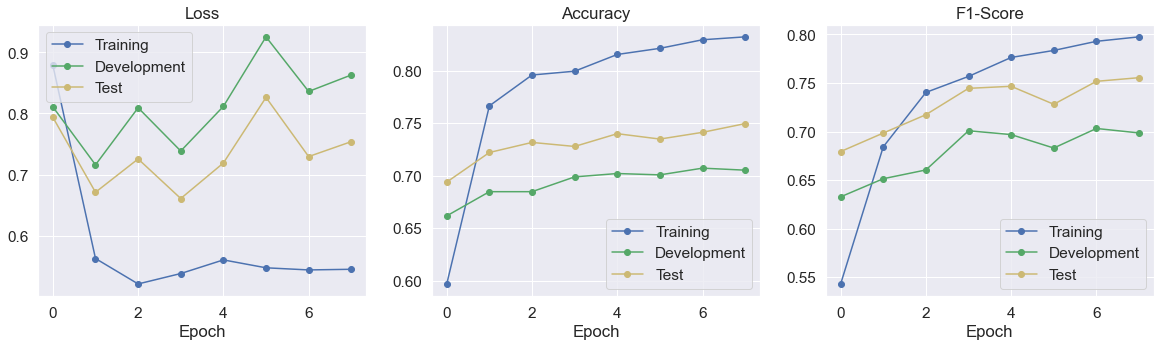
\includegraphics[width=0.9\linewidth]{images/metric_per_epoch.png}}
	\caption{عملکرد مدل آموزش دیده در هر 
	\lr{epoch} آموزش}
	\label{metric_per_epoch}
\end{figure}
در گام بعدی اثربخشی بخش‌های مهم روش پیشنهادی مورد بررسی دقیق‌تر قرار می‌گیرد. به صورت دقیق‌تر ‌تاثیر نوع پیش‌پردازش داده، افزایش دادگان آموزشی، رده‌بند و تابع ضرر بر نتایج نهایی  بررسی  می‌شود.

\subsection{گام سوم : ارزیابی تکمیلی مدل پیشنهادی}
در گام دوم با جستجو کامل بر روی همه پارامترهای مدل و ابرپارامترها، بهترین ترکیب پارامترها به دست آمد. پارامترهای نهایی مدل پیشنهادی در جدول~
\ref{best-config}
قابل مشاهده است. در این بخش با طراحی آزمایش‌هایی سعی شده تا تاثیر هر یک از موارد در نتیجه نهایی به صورت جداگانه بررسی شود.

\begin{table}[h!]
	\centering
	\small
	\caption{\label{best-config}پارامترهای بهترین مدل پیشنهادی.}
	\vspace{0.2cm}
	\begin{tabular}{c  |c }
		\hline
		پارامتر & مقدار\\
		\hline
		تعداد دوره
		 (\lr{Epoch})
	     & $8$ \\
		اندازه دسته (\lr{Batch Size}) & $4$\\
		نرخ یادگیری & $0.007903$\\
		طول عبارت ورودی & $128$ \\
		\lr{Dropout}  &  $0.5$\\
		\lr{Learning schedule} & 
		\lr{Linear Schedule With Warmup}
		\\
		\hline
		کدگذار & 
		\lr{BERTweet}
		\\
		رده‌بند & 
		\lr{CNN}
		\\
		\lr{N\_last\_layer} & $5$\\
		بهینه‌ساز & 
		\lr{SGD}
		\\
		تابع فعال‌سازی&
		 \lr{Weighted Cross Entropy}
		 \\
		\hline
		\hline
	\end{tabular}
	
	\centering
	
\end{table}


\subsubsection{اثربخشی نوع پیش‌پردازش داده}\label{sec:data-cleaning-impact}
برای تعیین میزان اثربخشی نوع پیش‌پردازش بر نتایج به دست آمده، آزمایش‌ها با بهترین پیکربندی تکرار شد (طبق پارامترهای جدول
\ref{best-config}).
در این آزمایش‌ها تنها نوع پیش‌پردارش تغییر کرده و پارامترهای مدل و ابرپارامترها ثابت هستند. برای هر تکنیک پیش‌پردازش، جهت اطمینان از نتایج به دست آمده، آزمایش‌ها 10 بار تکرار شدند. جدول
\ref{data-cleaning-impact}
نتایج به دست آمده را نشان می‌دهد.

\begin{table}[h!]
	\centering
	\small
	\caption[نتایج بررسی اثربخشی نوع پیش‌پردازش داده]
	{\label{data-cleaning-impact}
		نتایج بررسی اثربخشی نوع پیش‌پردازش داده. 
		علامت $\dagger$ نشان می‌دهد نتایج به دست آمده در مقایسه با روش پیش‌پردازش "نگهداشت داده‌های اصلی" به صورت معنی‌دار $(p < 0.005)$ بهتر هستند. علامت $\ast$ نشان‌ می‌دهد نتایج به دست آمده در مقایسه با روش پیش‌پردازش "تمیز کردن کامل داده‌ها" به صورت معنی‌دار $(p < 0.005)$ بهتر هستند.}
	
	\vspace{0.3cm}
	\begin{tabular}{c  |c }
		\hline
		روش پیش‌پردازش &
		 $F1-Score$
		 \\
		\hline
		نگهداشت داده‌های اصلی & $73.98 \pm 0.0012 ^\ast$\\
		حذف آدرس‌ اینترنتی & $73.92 \pm 0.0017 ^\ast$\\ 
		حذف نام‌کاربری & \textbf{$74.35 \pm 0.0015 ^\ast \dagger$} \\
		حذف همزمان نام کاربری و آدرس اینترنتی & $74.11 \pm 0.0029 ^\ast \dagger$\\
		حذف همزمان نام کاربری و آدرس اینترنتی و جدا کردن هشتک & $73.76 \pm 0.0014 ^\ast$\\
		حذف همزمان نام کاربری و آدرس اینترنتی و جدا کردن هشتک و کوچک کردن حروف
		 & $73.72 \pm 0.0009 ^\ast$\\
		تمیز کردن کامل داده‌ها
		 & $72.42 \pm 0.0020 $\\
		\hline
		\hline
	\end{tabular}	
\end{table}

 با ارزیابی مقدار
\lr{F1-Score}
به دست آمده می‌توان نتیجه گرفت روش "حذف نام‌کاربری" و "حذف همزمان نام کاربری و آدرس اینترنتی" در مقایسه با سایر روش‌ها بهترین نتیجه را کسب کردند. همچنین این روش‌ها به صورت معنادار از روش‌های "تمیز کردن کامل داده‌ها" و "نگهداشت داده‌های اصلی" بهتر است. مقدار $p-value$ به دست آمده در مقایسه این روش‌ها با سایر تکنیک‌ها کمتر از $0.0005$ می‌باشد که نشان می‌دهد بهبود معنادار
\LTRfootnote{Significance}
است. همچنین موثرترین روش پیش‌پردازش در مجموعه داده استفاده شده، حذف نام کاربری می‌باشد. علاوه بر این می‌توان گفت همه روش‌ها نسبت به روش "تمیز کردن کامل داده‌ها" نتایج بهتری کسب کردند. این بدان معنی است در این روش‌ ویژگی‌هایی
\LTRfootnote{Feature}
 از ورودی که می‌تواند تاثیر مثبتی بر عملکرد مدل داشته باشد حذف شده است. به عنوان مثال گاهی چندین علامت سوال یا علامت تعجب متوالی (!!!!، ؟؟؟؟؟) نشان دهنده یک حالت خاصی از تعجب یا عصبانیت و یا مخالفت است. اما در روش "تمیز کردن کامل داده‌ها"  با حذف علائم نگارشی، فرصت یادگیری با استفاده از این چنین موارد از مدل سلب می‌شود.

نمودار
~\ref{data-cleaning-impact-chart}
نشان می‌دهد از روش اول (نگهداشت داده‌های اصلی) تا روش سوم (حذف نام‌کاربری) تکنیک‌های پیش‌پردازش باعث بهبود مدل می‌شود. اما بعد از آن هر چه موارد بیشتری از متن ورودی حذف شود، عملکرد مدل به صورت معناداری کاهش می‌یابد. میانگین و بازه اطمینان مدل پیشنهادی در شکل~
\ref{data-cleaning-impact-bar-chart}
را برای انواع تکنیک‌های پیش‌پردازش نشان می‌دهد.

\begin{figure}[H]
	\center{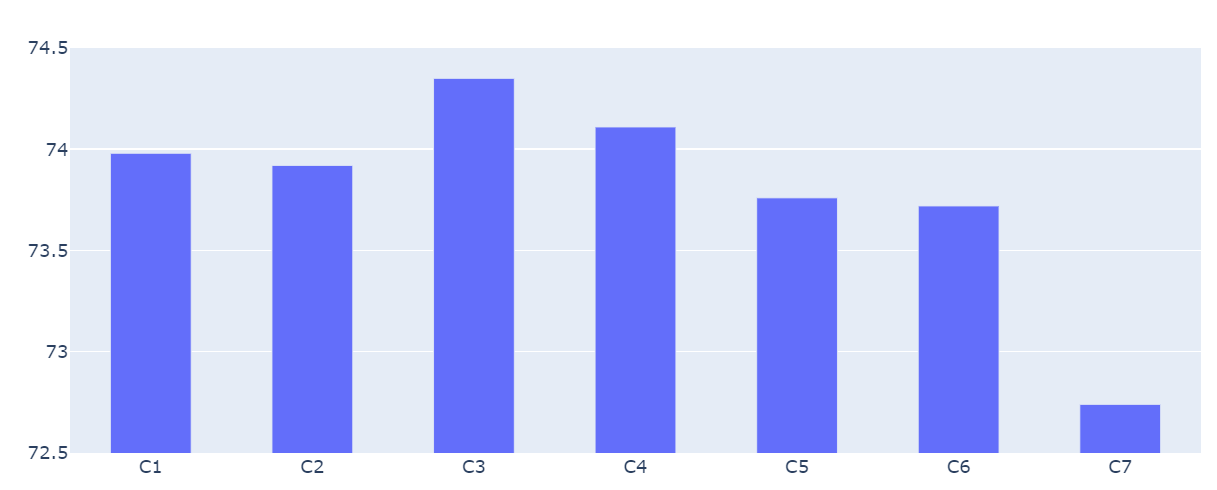
\includegraphics[width=0.9\linewidth]{images/data_cleaning_impact.png}}
	\caption{مقدار
	\lr{F1-Score}
هر یک از تکنیک‌های پیش‌پردازش داده}
	\label{data-cleaning-impact-chart}
\end{figure}

\begin{figure}[H]
	\center{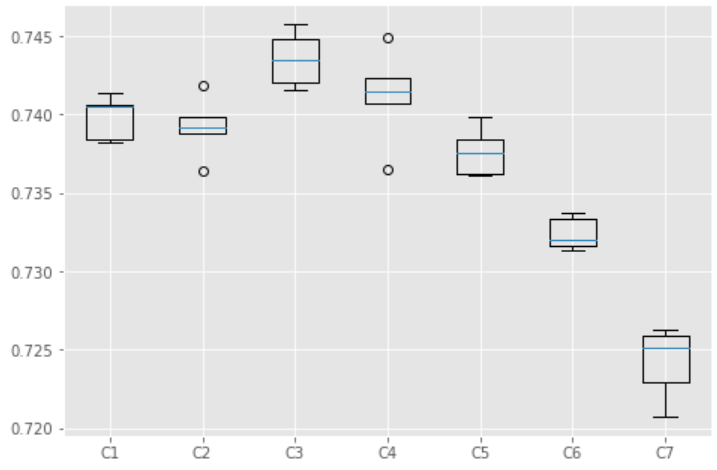
\includegraphics[width=0.6\linewidth]{images/data_cleaning_impact-box-chart-2.png}}
	\caption[بازه اطمینان مدل پیشنهادی بر اساس روش‌های پیش‌پردازش داده]{بازه اطمینان مدل پیشنهادی بر اساس روش‌های پیش‌پردازش داده بر حسب معیار
		\lr{F1-Score}}
	\label{data-cleaning-impact-bar-chart}
\end{figure}

\subsubsection{اثربخشی افزایش داده} \label{sec:data-aug-impact}
افزایش داده یکی از تکنیک‌های بهبود عملکرد مدل در مواجهه با مجموعه داده نامتوازن است. در این آزمایش همه پارامترها و فراپارامترهای مدل یکسان است و تنها داده‌های آموزشی تفاوت دارند. آزمایش‌ها به ازای داده‌های افزایش یافته و داده‌های اصلی 10 بار تکرار شدند. جدول
~\ref{data-aug-impact-table} 
تاثیر افزایش داده‌های آموزشی بر عملکرد نهایی مدل را نشان می‌دهد. بازه اطمینان مدل آموزش دیده با داده‌های افزایش یافته در شکل
~\ref{data-aug-impact-bar-chart}
نمایش داده شده است. همچنین برای بررسی دقیق‌تر، میزان تغییر معیارهای ارزیابی به ازای هر کلاس در جدول
~\ref{data-aug-impact-per-class}
نشان داده شده است. 
\begin{table*}[h!]
	
	\caption[نتایج بررسی اثربخشی افزایش داده. ]
	{\label{data-aug-impact-table}
		نتایج بررسی اثربخشی افزایش داده. علامت $\dagger$ نشان می‌دهد نتایج به دست آمده در مقایسه با حالت بدون افزایش داده به صورت معنی‌دار $(p < 0.05)$ بهتر هستند.}
	\centering
	\vspace{0.2cm}
	\begin{tabular}{c  c |c }
		\hline
		روش پیش‌پردازش&افزایش داده &  $F1-Score$\\
		\hline
		\multirow{2}{*}{حذف نام کاربری}&	-  & $74.11 \pm 0.0029$\\
										&  + & 	$74.79 \pm 0.0036 \dagger$\\
		\hline
		\hline
	\end{tabular}
	
\end{table*}

\begin{figure}[H]
	\center{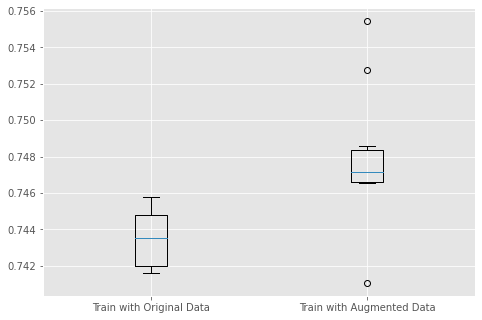
\includegraphics[width=0.6\linewidth]{images/data_aug_impact-box-chart.png}}
	\caption[بازه اطمینان مدل پیشنهادی آموزش دیده با داده‌های افزایش داده‌ شده]{بازه اطمینان مدل پیشنهادی آموزش دیده با داده‌های افزایش داده‌ شده بر حسب معیار
		\lr{F1-Score}}
	\label{data-aug-impact-bar-chart}
\end{figure}

\begin{table}[h!]
	\centering
	\centering
	\caption
	{\label{data-aug-impact-per-class}
		نتایج بررسی اثربخشی افزایش داده به ازای هر کلاس}
	\begin{tabular}{c  c |c c c}
		\hline
		افزایش داده & کلاس & 
		$Precision$ & $Recal$ &$F1-Score$
		\\
		\hline
		
		\multirow{3}{*}{-} & موافق &
		$76.33$ & $78.19$ & $77.25$ \\ 
		& مخالف &
		$75.17$ & $93.80$ & $83.48$ \\ 
		& بدون نظر &
		$62.6$ & $56.90$ & $59.61$ \\ 
		\hline
		\multirow{3}{*}{+} & موافق &
		$81.54$ & $77.58$ & \underline{$79.51$} \\ 
		& مخالف &
		$76.59$ & $95.57$ & \underline{$85.39$} \\ 
		& بدون نظر &
		$59.80$ & $61.16$ & \underline{$60.95$} \\ 
		
		\hline
		\hline
	\end{tabular}
	
	
\end{table}

با بررسی نتایج می‌توان گفت افزایش داده‌های آموزشی عملکرد نهایی مدل را به صورت معناداری بهبود داده است. همچنین با بررسی 
\lr{F1-Score}
به ازای هر کلاس می‌توان گفت پیش‌بینی همه کلاس‌ها نیز بهبود قابل قبولی داشتند. بدین ترتیب مدل با دیدن توزیع مناسبی از داده‌ها در زمان آموزش، عملکرد مناسب‌تری در زمان ارزیابی از خود نشان داده است. همچنین می‌توان نتیجه گرفت تکنیک انتخاب شده برای افزایش داده (بخش
~\ref{sec:dataaug})
داده‌های با کیفیتی تولید کرده است.

\subsubsection{اثربخشی رده‌بند}

در این بخش میزان اثربخشی نوع رده‌بند در عملکرد مدل را مورد بررسی قرار گرفت. از آنجا که طبق نتایج جدول
\ref{data-cleaning-impact}
دو سطح از پیش‌پردازش به صورت معنادار از بقیه روش‌ها بهتر بودند، آزمایش‌های این بخش تنها با دو روش پیش‌پردازش تکرار شد. همچون قسمت قبل، پارامترهای مدل و ابرپارامترها ثابت هستند و تنها نوع رده‌بند تغییر می‌کند. علاوه بر این جهت اطمینان از نتایج به دست آمده، آزمایش‌ها  10 بار تکرار شد. جدول
\ref{classifier-impact}
نتایج به دست آمده را نشان می‌دهد.

\begin{table*}[h!]
	
		\caption[		نتایج بررسی اثربخشی رده‌بند]
	{\label{classifier-impact}
		نتایج بررسی اثربخشی رده‌بند. علامت $\dagger$ نشان می‌دهد نتایج به دست آمده در مقایسه با رده‌بند \lr{FNN} به صورت معنی‌دار $(p < 0.05)$ بهتر هستند.}
	\centering
	\vspace{0.2cm}
	\begin{tabular}{c  c |c }
		\hline
		رده‌بند & روش پیش‌پردازش& $F1-Score$\\
		\hline
		
		\multirow{2}{*}{\lr{CNN}} & حذف نام‌کاربری &\textbf{$74.35 \pm 0.0015 \dagger
			$ } \\ 
				& حذف همزمان نام کاربری و آدرس اینترنتی &
				 $74.11 \pm 0.0029$\\
		\hline
		\multirow{2}{*}{\lr{FNN}} & حذف نام‌کاربری &$73.73 \pm 0.0058$ \\
		 &حذف همزمان نام کاربری و آدرس اینترنتی
		  & $73.91 \pm 0.0045$\\
		
		\hline
		\hline
	\end{tabular}
	
\end{table*}

نتایج نشان می‌دهد رده‌بند ساخته شده با شبکه عصبی پیچشی 
(\lr{CNN})
به صورت معناداری از رده‌بند شبکه عصبی تماما متصل عملکرد بهتری دارد. از آنجا که رده‌بند 
\lr{CNN}
کانولوشن‌هایی با سایزهای مختلف و به صورت موازی اعمال می‌کند، احتمال یادگیری از همسایگی با سایزهای مختلف را پیدا کرده و عملکرد بهتری از خود نشان می‌دهد.
\subsubsection{اثربخشی تابع ضرر}
جدول
\ref{loss-functoion-impact}
تاثیر تغییر تابع ضرر بر نتایج مدل نهایی را نمایش می‌دهد. آزمایش‌های این بخش به ازای هر یک از تنظیمات 10 بار تکرار شدند. سایر پارامترها و اپر پارامترهای مدل ثابت می‌باشد (طبق جدول~
\ref{best-config}).

\begin{table}[h!]
	\centering
	\small

	\caption[نتایج بررسی اثربخشی تابع ضرر بر حسب
	\lr{F1-Score}
	.]{نتایج بررسی اثربخشی تابع ضرر بر حسب
		\lr{F1-Score}. 
	علامت $\dagger$ نشان می‌دهد نتایج به دست آمده در مقایسه با تابع ضرر \lr{Weighted Cross Entropy} به صورت معنی‌دار $(p < 0.05)$ بهتر هستند.
\lr{Cross Entropy}
به اختصار
\lr{CE}
نوشته شده است.
	 	\label{loss-functoion-impact}}
\vspace{0.2cm}
\begin{tabular}{c  |c | c | c}
	\hline
	روش پیش‌پردازش 
	&Focal
	&\lr{Weighted CE}
	& \lr{Weighted CE + Focal}
	\\
	\hline
	نگهداشت داده‌های اصلی &
	$73.95 \pm 0.0034$
	&$73.98 \pm 0.0012$
 	& $74.15 \pm 0.0035$\\

	حذف آدرس‌ اینترنتی &
	$74.03 \pm 0.0011 $
	& $73.92 \pm 0.0017$
	 &  $74.01 \pm 0.0021$
	 \\ 
	حذف نام‌کاربری & 
	$74.13 \pm 0.0015 $
	&\textbf{$74.35 \pm 0.0015$} 
	& $74.31 \pm 0.0031$
	\\
	حذف نام کاربری و آدرس اینترنتی &
	$73.14 \pm 0.0032$
	&$74.11 \pm 0.0029$
	&  $74.35 \pm 0.0025$
	\\
	تمیز کردن کامل داده‌ها&
    $73.12 \pm 0.0028$
	& $72.42 \pm 0.0020 $
	& $73.03 \pm 0.0035 ^\dagger$\\

	\hline
	\hline
\end{tabular}	
\end{table}

همان‌طور که مشخص است استفاده از جمع دو تابع ضرر
\lr{Focal}
و
\lr{Weighted Cross Entropy}
عمکلرد بهتری نسبت به استفاده از یکی از آن‌ها دارد. برای حالت پیش‌پردازش "تمیز کردن کامل داده‌ها" این بهبود معنادار است. در این حالت مقدار $p-value$ به دست آمده کوچکتر $0.05$ می‌باشد. در سایر موارد با مقایسه مقدار
\lr{F1-Score}
می‌توان گفت مدل بهبود داشته اما این بهبود معنی‌دار نمی‌باشد.
\iffalse
\begin{table*}[h!]	
	\caption[ نتایج بررسی اثربخشی پارامتر گاما با روش پیش‌پردازش حذف نام کاربری]
	{\label{focal-gamma-impact}
		نتایج بررسی اثربخشی پارامتر گاما با روش پیش‌پردازش حذف نام کاربری}
	\centering
	\vspace{0.2cm}
	\begin{tabular}{ c |c }
		\hline
		مقدار گاما&
			  $F1-Score$\\
    	\hline
		1 & $74.58$ \\
		2 & $74.14$\\
		3 & $74.01$\\
		4 & \\
		5 & $74.45$\\  
		\hline
		\hline
	\end{tabular}
	
\end{table*}
\fi

\subsubsection{بررسی تاثیر دامنه بر نتایج مدل آموزش دیده}
یکی دیگر از بررسی‌های صورت گرفته میزان 
\lr{Domain Specefic}
بودن مدل آموزش دیده می‌باشد. برای بررسی دقیق‌تر، دو موضوع تغییرات آب‌ و هوایی و قانونی شدن سقط جنین از مجموعه داده
\lr{SemEval-2016}
انتخاب شدند. به این منظور مدل‌های آموزش دیده بر روی مجموعه داده 
\lr{ClimaConvo}
بر دو قسمت از مجموعه داده 
\lr{SemEval2016}
مورد ارزیابی قرار گرفتند. نتایج به دست آمده در جدول~
\ref{domain-specefic}
قابل مشاهده است.

\begin{table}[h!]
	\centering
	\small
	\caption
	{\label{domain-specefic}
		بررسی تاثیر دامنه بر نتایج مدل آموزش دیده بر اساس معیار
		\lr{F1-Score}.}
	\vspace{0.2cm}
	\begin{tabular}{ c | c |c | c}
		\hline
		روش پیش‌پردازش & 
		\lr{ClimaConvo}
		&\lr{SemEval-CC}
		& \lr{SemEval-LA}
		\\
		\hline
		نگهداشت داده‌های اصلی &
		$73.98 \pm 0.0012$&
		$30.89 \pm 0.0216$ &
		$29.65 \pm 0.0142$\\
		
		حذف آدرس‌ اینترنتی &
		$73.92 \pm 0.0017$
		& $29.97 \pm 0.0231$
		& $31.05 \pm 0.0074$ \\ 
		حذف نام‌کاربری & 
		\textbf{$74.35 \pm 0.0015$} 
		& $30.53 \pm 0.0215$
		& $29.11 \pm 0.0104$
		\\
		حذف همزمان نام کاربری و آدرس اینترنتی & 
		$74.11 \pm 0.0029$
		& $30.34 \pm 0.0187$
		& $30.40 \pm 0.0088$
		\\
		تمیز کردن کامل داده‌ها
		& $72.42 \pm 0.0020 $
		& $30.18 \pm 0.0328 $
		& $29.05 \pm 0.0142 $
		\\
		
		\hline
		\hline
	\end{tabular}	
\end{table}

در مجموعه داده 
\lr{SemEval}
تاثیر نوع پیش‌پردازش کمتر می‌باشد. همچنین موضوع مجموعه داده
\lr{ClimaConvo}
و 
\lr{SemEval-CC}
یکسان است اما عملکرد مدل بر روی آن بسیار ضعیف است.  به نظر می‌رسد گذر زمان باعث شده مدل آموزش دیده بر روی مجموعه داده 
\lr{ClimaConvo}
بر مجموعه داده 
\lr{SemEval-CC}
عملکرد مناسبی نداشته باشد. به عبارت دیگر گذر زمان موجب تغییر در نوع داده‌ها شده و بنابراین مدل آموزش دیده بر داده‌های جدید (جمع‌آوری شده در سال 2022)  مناسب داده‌های قدیمی جمع‌آوری شده (در سال 2016) نمی‌باشد.
از طرف دیگر عملکرد مدل بر موضوع قانونی شدن سقط جنین چندان مناسب نیست. به طور کلی می‌توان گفت مدل برای داده‌های با موضوع و توزیع متفاوت نمی‌تواند عملکرد مناسبی داشته باشد. 
\subsection{تحلیل خطا}
با تحلیل خروجی به دست آمده می‌توان گفت مدل در پیشبینی کلاس بدون نظر ضعیف است. شکل
\ref{confusion_matrix}
نشان می‌دهد که در در 209 نمونه کلاس موافق به اشتباه بدون نظر پیشبینی شده است. همچنین در 149 نمونه کلاس بدون نظر به اشتباه موافق پیشبینی شده است. همچنین گاهی در عبارات کلاس مخالف که در قالب طعنه یا کنایه مطرح شده، مدل در تشخیص کلاس درست دچار خطا میشد. در این نوع توییت، نویسنده متن با کنایه مخالفت خود را نسبت به موضوع اهمیت تغییرات اقلیمی بیان می‌کند. در حالی که مدل نتوانسته بود این موضوع را به درستی درک کند. در جدول
\ref{error-example}
نمونه‌ای از اشتباهات در خروجی قابل مشاهده است.


\begin{figure}[H]
	\center{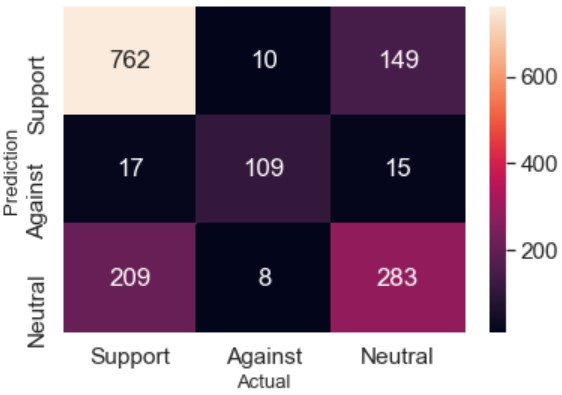
\includegraphics[width=0.5\linewidth]{images/confusion_matrix.jpg}}
	
	\caption{ماتریس درهمریختگی برای داده ارزیابی مجموعه
		\lr{ClimaConvo}}
	\label{confusion_matrix}
\end{figure}

\begin{table}[h!]
	\small
	\caption{چند نمونه  پیشبینی‌های اشتباه مدل}
	\label{error-example}
	\centering
	\vspace{0.2cm}
	\begin{tabular}{c | c c c}
		\lr{\ }
		متن توییت & نوع خطا & کلاس اصلی & کلاس پیش‌بینی شده
		\\
		\hline
		
		\begin{tabular}{@{}c@{}}
			\lr{\#FridaysForFuture \#ClimateChange\#ExtinctionRebellion} \\ 
			\lr{\#GlobalWarming What are we saving?}\\
		\end{tabular}
		& کنایه & مخالف& بدون نظر
		\\
		\hline
		\hline
	\end{tabular}
	
\end{table}

برای بررسی کامل‌تر علت خطاهای مدل، با استفاده از ابزار
\lr{Transformers Interpret} \LTRfootnote{\href{https://github.com/cdpierse/transformers-interpret}{https://github.com/cdpierse/transformers-interpret}}
تحلیلی از خروجی تولید شده توسط مدل صورت گرفت. شکل
\ref{error-analysis}
دو مثال از پیشبینی صحیح مدل را نشان می‌دهد. رنگ سبز نشان‌ می‌دهد که برای پیش‌بینی کلاس نهایی، توجه بیشتری به آن کلمه شده است. نکته قابل توجه این است که برای هر دو خروجی مدل توانسته به کلمات تاثیرگذار توجه کند. به عبارت دیگر مدل کلمات مهم و تاثیرگذار برای فهم متن را توانسته به درستی تشخیص دهد. بنابراین همان‌طور که انتظار می‌رفت پیشبینی مدل نیز صحیح می‌باشد.  در مقابل گاهی کلمات مورد توجه مدل برای پیشبینی صحیح کافی نیست. به عبارت دیگر نیاز به فهم بیشتری دارد. در شکل
\ref{error-analysis-wrong-answers}
دو نمونه از پیشبینی نادرست مدل مشاهده می‌شود. در مثال دوم اگر کلمات
\lr{dying}
و 
\lr{don't care}
نیز مورد توجه مدل قرار می‌گرفت، احتمال پیشبینی درست توسط مدل افزایش می‌یافت.

\begin{figure}[H]
	\center{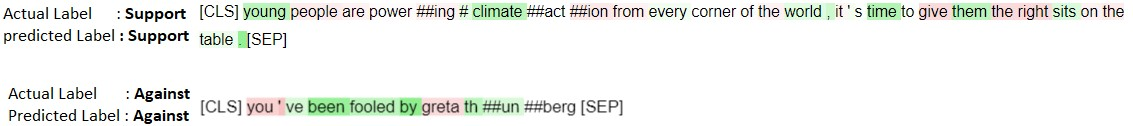
\includegraphics[width=1\linewidth]{images/TransformersInterpretTruePredictedLabel.jpg}}
    \vspace{-1cm}
	\caption{خروجی میزان توجه مدل به کلمات ورودی برای پیشبینی‌های درست}
	\label{error-analysis}
\end{figure}

\begin{figure}[H]
	\center{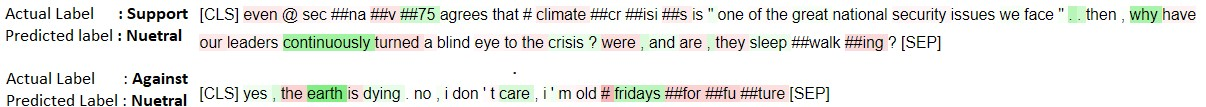
\includegraphics[width=1\linewidth]{images/TransformersInterpretFalsePredictedLabel.jpg}}
	\vspace{-1cm}
	\caption{خروجی میزان توجه مدل به کلمات ورودی برای پیشبینی‌های اشتباه}
	\label{error-analysis-wrong-answers}
\end{figure}


\subsection{مزایا و معایب روش پیشنهادی}
روش پیشنهادی حل مسئله شامل یک تکنیک گام به گام برای طراحی معماری پیشنهادی و بررسی اثربخشی آن است. با توجه به فضای جستجو بررسی شده، می‌توان گفت این روش توانست به نتایج بسیار قابل قبولی دست پیدا کند. همچنین تعریف فضای جستجو به صورت مناسب نیز از دیگر دلایل موفقیت روش پیشنهادی است (استفاده از 
\lr{CNN}
در رده‌بند). از سوی دیگر بررسی انواع پیش‌پردازش متن در اکثر پژوهش‌ها مورد غفلت واقع می‌شود. اما مزیت این پژوهش توجه به روش پیش‌پردازش و برررسی انواع آن است.

از جمله معایب روش ارائه شده نیاز به داده آموزشی کافی برای آموزش مدل می‌باشد. از طرف دیگر طبق بررسی‌های انجام شده، مدل آموزش دیده
\lr{Domain Specific}
می‌باشد و عملکرد مناسبی در سایر دامنه‌ها که در آن آموزش داده نشده، از خود نشان نداده است. وجود 
\lr{GPU}
با رم مناسب برای آموزش مدل‌ها ضروری است.



\subsection{نحوه پیاده‌سازی و اجرا آزمایش‌ها}
پیاده‌سازی پروژه در 
\href{https://github.com/ghazaleh-mahmoodi/Climate_Activism_Stance_Detection}{اینجا}
\LTRfootnote{\href{https://github.com/ghazaleh-mahmoodi/Climate_Activism_Stance_Detection}{https://github.com/ghazaleh-mahmoodi/Climate\_Activism\_Stance\_Detection}}
قابل مشاهده می‌باشد که با زبان پایتون و فریم‌ورک پارتورچ انجام شده است. برای اجرا آزمایش‌ها لازم است با دستور 
\lr{pip3 install -r requirements.txt}
پکیج‌های مورد نیاز برای اجرا کد را نصب کنید. با توجه به طولانی بودن زمان اجرا کل آزمایش‌ها بهتر است با دستور 
\lr{screen}
یک اسکرین جدید برای اجرا بسازید و به شکل معمول دستورات را اجرا کنید. در این صورت حتی با بستن ترمینال اجرا ادامه پیدا می‌کند. با
\lr{screen -r}
در صورت باز کردن مجدد ترمینال می‌توانید فرآیند و میزان پیشرفت اجرا را ببینید.
راه حل دیگر برای تداوم اجرا در صورت بستن ترمینال استفاده از دستور 
\lr{nohup}
است. کافیست
\lr{nohup bash stance\_run.bash}
را اجرا کنید. خروجی‌های اجرا در 
\lr{nohup.out}
قابل مشاهده می‌باشد.
\newline
در صورتی که یک
\lr{screen}
جدید برای خود ساختید، با دستور
\lr{bash stance\_run.bash}
کلیه آزمایش‌ها به صورت متوالی اجرا می‌شود. در نهایت نتایج به دست‌آمده در پوشه 
\lr{result}
ذخیره می‌شود. همچنین وزن‌های شبکه در پوشه
\lr{models}
قابل مشاهده می‌باشند.
\newline
برای اجرا از سخت‌افزار
\lr{GPU.1080Ti.xlarge}
با رم 
\lr{31.3GB}
استفاده شد. دستور 
\lr{nvidia-smi}
میزان استفاده از 
\lr{GPU}
را نمایش می‌دهد. خروجی این دستور در هنگام آموزش مدل به صورت شکل \ref{nvidia-smi} شد.
\begin{figure}[H]		  		    			  	 \center{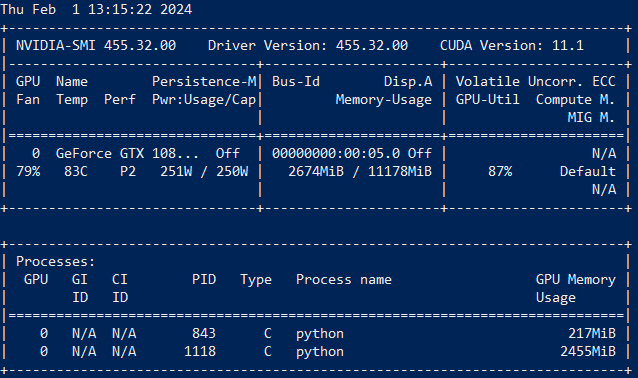
\includegraphics[width=0.8\linewidth]{images/nvidia-smi.jpg}}
	\caption{میزان مصرف \lr{GPU}در زمان آموزش مدل پیشنهادی}
	\label{nvidia-smi}
\end{figure}

\section{جمع‌بندی}
در این فصل به مسئله تشخیص موضع با نظارت پرداخته شد. ابتدا مجموعه داده‌های مورد استفاده معرفی شدند. در ادامه روش حل مسئله شامل تعریف اتولع حالات پیش‌پردازش داده، نحوه افزایش داده، روش جستجو برای معماری و ابرپارامترها و مثادیر فضای جستجو به صورت مفصل بیان شد. در انتها برای بررسی تاثیر نحوه پیش‌پردازش، افزایش داده، رده‌بند و تابع ضرر آزمایش‌های اصولی طراحی و انجام شد. در فصل بعد به مسئله تشخیص موضع بدون داده آموزشی پرداخته می‌شود.


% !TeX root=main.tex
\iffalse
% You can copy any following box you like to your code.
\newtcolorbox{boxA}{
	fontupper = \bf,
	boxrule = 1.5pt,
	colframe = black % frame color
}

\begin{boxA}
	\lr{The box area is made visible by the shadow instead of the border. The top line may be placed on the left (replace border-top with border-left).}
\end{boxA}

\newtcolorbox{boxM}{
	fontupper = \color{white},
	rounded corners,
	arc = 6pt,
	colback = main!80, 
	colframe = main, 
	boxrule = 0pt, 
	bottomrule = 4.5pt,
	enhanced,
	fuzzy shadow = {0pt}{-3pt}{-0.5pt}{0.5pt}{black!35}
}
\begin{boxM}
	\lr{I added a shadow to give it a more three-dimensional appearance. It's a little flashy, so it might be good to use it on the part you really want to stand out.}
\end{boxM}
\fi


\chapter{روش پیشنهادی برای تشخیص موضع بدون داده آموزشی}

\setlength\parindent{0pt}   % killing indentation for all the text
\setstretch{1.3}            % setting line spacing to 1.3
\setlength\columnsep{0.25in} % setting length of column separator
\pagestyle{empty}           % setting pagestyle to be empty


\definecolor{main}{HTML}{5989cf}    % setting main color to be used
\definecolor{sub}{HTML}{cde4ff}     % setting sub color to be used

\newtcolorbox{boxK}{
	sharpish corners, % better drop shadow
	boxrule = 0pt,
	toprule = 4.5pt, % top rule weight
	enhanced,
	fuzzy shadow = {0pt}{-2pt}{-0.5pt}{0.5pt}{black!35} % {xshift}{yshift}{offset}{step}{options} 
}

\definecolor{ao(english)}{rgb}{0.0, 0.5, 0.0}
\definecolor{vividauburn}{rgb}{0.58, 0.15, 0.14}
\thispagestyle{empty}


امروزه استفاده از مدل‌های زبانی بزرگ برای حل مسائل مختلف پردازش زبان طبیعی بسیار فراگیر شده است. با استفاده از این مدل‌ها می‌توان بدون داده آموزشی یا با داده آموزشی کم و با طراحی یک پرامپت مناسب
\LTRfootnote{Prompt Engineering}
 نتایج قابل قبولی به دست آورد. در این پژوهش، به منظور استفاده از مدل‌های زبانی بزرگ در مسئله تشخیص موضع، چهار پرامپت با رویکردهای متفاوت پیشنهاد شد. پرامپت‌ها به صورت سلسله مراتبی تعریف شدند. بدین معنا که هر پرامپت اطلاعات بیشتری نسبت به پرامپت قبلی به عنوان ورودی دریافت می‌کنند. در ادامه هر یک از رویکردهای پیشنهادی به تفصیل توضیح داده می‌شود.


\section{روش حل مسئله}
در این پژوهش 4 پرامپت در سطح‌های متفاوت تعریف شدند. در طراحی پرامپت از قواعد پیشنهاد شده توسط بزرگ‌ترین توسعه دهندگان مدل‌های زبانی بزرگ (همچون 
\lr{OpenAI}) استفاده کردیم
\LTRfootnote{\href{https://platform.openai.com/docs/guides/prompt-engineering/six-strategies-for-getting-better-results}{https://platform.openai.com/docs/guides/prompt-engineering/six-strategies-for-getting-better-results}}.
اصول استفاده شده در طراحی پرامپت عبارتند از:
\begin{enumerate}
	\item نوشتن درخواست به صورت ساده و واضح و دقیق: باید ورودی و خروجی و مسئله‌ای که مدل قصد حل کردن آن را دارد به صورت کاملا واضح و شفاف توضیح داده شود. هر چه قدر توضیحات دقیق‌تر و کامل‌تری در پرامپت  باشد، احتمال رسیدن به پاسخ صحیح بیشتر می‌شود. همچنین مشخص کردن دقیق خروجی درخواستی از مدل، باعث بهبود نتایج می‌شود. وجود چند مثال از حل مسئله (رویکرد
\lr{Few Shot}\cite{10.5555/3495724.3495883}) 
نیز می‌تواند ایده مناسبی برای بهره‌مندی بیشتر مدل از پرامپت ورودی باشد.

\item تقسیم کردن مسئله اصلی به چند زیر مسئله ساده‌تر: نرخ پاسخگویی اشتباه در مسائل پیچیده بسیار بالاست. بنابراین یک راه حل بهینه این است که مسئله اولیه، در قالب چند زیر مسئله ساده‌تر تعریف شود. در ادامه گام‌های حل هر مسئله به صورت شفاف توضیح داده‌ شود تا احتمال رسیدن به پاسخ مطلوب افزایش یابد (رویکرد
\lr{Chain of Thought}
از این قاعده استفاده می‌کند). در این صورت به مدل زمان لازم برای استنتاج داده می‌شود و پاسخ‌های قابل اعتمادتری تولید می‌شود.
\end{enumerate}

با توجه به اصول مطرح شده به عنوان راهنما برای طراحی پرامپت، چهار پرامپت در سطوح مختلف با رویکرد‌های متفاوت تعریف شدند. در ادامه به توضیح چهار پرامپت پیشنهادی این پژوهش پرداخته می‌شود.

\subsection{پرامپت
\lr{Zero Shot}
}
در این پرامپت ساده‌ترین روش در نظر گرفته شد. پرامپت متشکل از توضیح مسئله، وظیفه خواسته شده از مدل، ورودی‌های مسئله تشخیص موضع شامل موضوع
\LTRfootnote{Target}
و متن توییت و مشخص نمودن کلاس‌های خروجی می‌باشد. در نوشتن پرامپت توضیحات به صورت دقیق و ساده ارائه شدند. شکل
\ref{zeroshot-prompt}
قالب پیشنهادی را نشان می‌دهد. 

\begin{figure}[H]
	\small
	\begin{boxK}
		\raggedright
		\lr{{The following statements (tweet) are twitter posts about {target}    target. Each statement can support, oppose, or be neutral toward its associated {target} belief and Each statement has the reason for that stance.}}\\
		\lr{Now, classify the following statement as to whether support, oppose, and neutral toward the belief below being true, and give your explanation for the classification.}\\
		\lr{Target: \texttt{<target>}}\\
		\lr{Tweet: \texttt{<tweet?}}\\
		\lr{Stance : {{select 'Stance' ['support', 'oppose', 'neutral'] }}}\\
		\lr{Explanation: {{gen 'explanation'}}}
	\end{boxK}
	\caption{\label{zeroshot-prompt}الگو پرامپت \lr{Zero Shot}}
\end{figure}

\subsection{پرامپت
	\lr{Zero Shot + Chain of Thought}
}
این رویکرد، در ادامه پرامپت
\lr{Zero Shot}
پیشنهاد شده است. در این پرامپت توضیحات مربوط به نحوه حل مسئله گام به گام توضیح داده شده به طوری که مدل زمان لازم برای استدلال را داشته باشد. همچنین با تقسیم مسئله به زیر مسئله‌های ساده‌تر مدل برای دستیابی به پاسخ صحیح راهنمایی می‌شود. شکل
\ref{zeroshot-Cot-prompt}
قالب پیشنهادی را نشان می‌دهد. قسمت مربوط به 
\lr{Chain of Thought (CoT)}
با رنگ 
\textcolor{blue}{آبی}
 مشخص شده است.
\begin{figure}[H]
	\small
	\begin{boxK}
		\raggedright
		\lr{{The following statements (tweet) are twitter posts about {target}    target. Each statement can support, oppose, or be neutral toward its associated {target} belief and Each statement has the reason for that stance.}}\\
		\lr{Now, classify the following statement as to whether support, oppose, and neutral toward the belief below being true, and give your explanation for the classification.}\\
		\lr{\textcolor{blue}{let's think step by step.}}\\
		\lr{\textcolor{blue}{First, check if the author of the tweet has commented on climate change. Has he commented at all? Then check if the author supports that climate change is a concern and should be addressed. Or is the author's opinion that this matter does not require special attention?}}\\
		\lr{Target: $<target>$}\\
		\lr{Tweet: \texttt{$<tweet>$}}\\
		\lr{Stance : {{select 'Stance' ['support', 'oppose', 'neutral'] }}}\\
		\lr{Explanation: {{gen 'explanation'}}}
	\end{boxK}
	\caption{\label{zeroshot-Cot-prompt}الگو پرامپت \lr{Zero Shot + Chain of Thought}}
\end{figure}


\subsection{پرامپت
\lr{Zero Shot + Chain of Thought + Context Description}
}

این پرامپت، در ادامه پرامپت
\lr{Zero Shot + Chain of Thought}
پیشنهاد شد. نقطه ضعف پرامپت‌های قبلی عدم وجود توضیحاتی راجع به موضوع تغییرات اقلیمی است و تنها تعریف مسئله تشخیص موضع در متن پرامپت وجود دارد. در این پرامت سعی شده توضیحاتی راجع به موضوع مورد بحث نیز به عنوان ورودی در نظر گرفته شود. توضیحات برگرفته از صفحه ویکی‌پدیا مربوطه می‌باشد. شکل
\ref{zeroshot-Cot-Context Description-prompt}
قالب پیشنهادی را نشان می‌دهد. قسمت مربوط به 
\lr{Context}
با رنگ
\textcolor{ao(english)}{سبز}
 مشخص شده است.
\begin{figure}[H]
	\small
	\begin{boxK}
		
		\raggedright
		\lr{The following statements (tweet) are twitter posts about Climate Change.	\textcolor{ao(english)}{Climate change describes global warming—the ongoing increase in global average temperature—and its effects on Earth's climate system. Climate change in a broader sense also includes previous long-term changes to Earth's climate.  Fossil fuel use, deforestation, and some agricultural and industrial practices add to greenhouse gases, notably carbon dioxide and methane. Greenhouse gases absorb some of the heat that the Earth radiates after it warms from sunlight.}
		 Each statement can support, oppose, or be neutral toward its associated {target} belief and Each statement has the reason for that stance.}\\
		\lr{Now, classify the following statement as to whether support, oppose, and neutral toward the belief below being true, and give your explanation for the classification.}\\
		\lr{\textcolor{blue}{let's think step by step.}}\\
		\lr{\textcolor{blue}{First, check if the author of the tweet has commented on climate change. Has he commented at all? Then check if the author supports that climate change is a concern and should be addressed. Or is the author's opinion that this matter does not require special attention?}}\\
		\lr{Target: \texttt{$<target>$}}\\
		\lr{Tweet: \texttt{$<tweet>$}}\\
		\lr{Stance : {{select 'Stance' ['support', 'oppose', 'neutral'] }}}\\
		\lr{Explanation: {{gen 'explanation'}}}
	\end{boxK}
	\caption{\label{zeroshot-Cot-Context Description-prompt}الگو پرامپت \lr{Zero Shot + Chain of Thought + Context Description}}
	
\end{figure}
\subsection{پرامپت
	\lr{Few Shot + Chain of Thought + Context Description}
}
تا این مرحله اطلاعات مناسبی به متن پرامپت ورودی اضافه شد. پرامپت پیشنهاد شده در این مرحله از رویکرد
	\lr{Few Shot + Chain of Thought + Context Description}
	پیروی می‌کند. در این پرامپت علاوه بر ورودی‌های قبلی، چند مثال از متن توییت و موضع توییت آورده شده است. در این روش سعی شده با دیدن چند نمونه آموزشی، بهبودی در عملکرد مدل ایجاد کنیم. شکل
	\ref{fewshot-Cot-Context Description-prompt}
	قالب پیشنهادی را نشان می‌دهد. نمونه‌های آموزشی در این پرامپت به صورت تصادفی انتخاب شدند. قسمت مربوط به 
	\lr{Few Shot}
	با رنگ
 \textcolor{vividauburn}{قهوه‌ای}
	  مشخص شده است.


\begin{figure}[H]
	\scriptsize
	\begin{boxK}
		\raggedright
		\lr{The following statements (tweet) are twitter posts about Climate Change.	\textcolor{ao(english)}{Climate change describes global warming—the ongoing increase in global average temperature—and its effects on Earth's climate system. Climate change in a broader sense also includes previous long-term changes to Earth's climate.  Fossil fuel use, deforestation, and some agricultural and industrial practices add to greenhouse gases, notably carbon dioxide and methane. Greenhouse gases absorb some of the heat that the Earth radiates after it warms from sunlight.} Each statement can support, oppose, or be neutral toward its associated {target} belief and Each statement has the reason for that stance.}\\
		\lr{\textcolor{vividauburn}{Let's see some example.}}\\
		\lr{\textcolor{vividauburn}{the tweet \texttt{$<tweet>$} stance on Climate change is supportive.}}\\
		\lr{\textcolor{vividauburn}{the tweet \texttt{$<tweet>$} stance on Climate change is opposite.}}\\
		\lr{\textcolor{vividauburn}{the tweet \texttt{$<tweet>$} stance on Climate change is neutral.}}\\
		\lr{Now, classify the following statement as to whether support, oppose, and neutral toward the belief below being true, and give your explanation for the classification.}\\
		\lr{\textcolor{blue}{let's think step by step}}\\
		\lr{\textcolor{blue}{First, check if the author of the tweet has commented on climate change. Has he commented at all? Then check if the author supports that climate change is a concern and should be addressed. Or is the author's opinion that this matter does not require special attention?}}\\
		\lr{Target: \texttt{$<target>$}}\\
		\lr{Tweet: \texttt{$<tweet>$}}\\
		\lr{Stance : {{select 'Stance' ['support', 'oppose', 'neutral'] }}}\\
		\lr{Explanation: {{gen 'explanation'}}}
	\end{boxK}
	\caption{\label{fewshot-Cot-Context Description-prompt}الگو پرامپت \lr{Few Shot + Chain of Thought + Context Description}}
\end{figure}

\section{آزمایش‌ها و تحلیل نتایج}
برای انجام آزمایش‌ها از مجموعه داده
\lr{ClimaConvo}\cite{shiwakoti2024analyzing}
و
\lr{SemEval}\cite{mohammad-etal-2016-semeval}
و مدل
\lr{Orca}\cite{orca-mini-v3-7b}
استفاده شد. به دلیل عملکرد مناسب مدل 
\lr{Orca}
در مقایسه با سایر مدل‌هایی با تعداد پارامتر مشابه از این مدل برای اجرا آزمایش‌ها استفاده شد (با توجه به سخت‌افزار موجود امکان استفاده از مدل‌های زبانی با پارامترهای بیشتر میسر نیست). در اجرا آزمایش‌ها پارامتر دما
\LTRfootnote{Temperature}
برابر با صفر قرار گرفت تا همواره توکن با بیشترین احتمال را تولید کند. از آن‌جایی که نتایج مدل‌های
\lr{Zero Shot}
برای مجموعه داده 
\lr{SemEval}
موجود بود، ابتدا مقایسه‌ای از روش‌های موجود شامل تکنیک‌های یادگیری عمیق و پرامپت با روش معرفی شده انجام شد. در جدول
~\ref{prompt-result-semeval}
پرامپت‌های پیشنهادی با سایر روش‌های یادگیری عمیق با رویکرد یادگیری بدون داده آموزشی مورد مقایسه قرار گرفت. نتایج به دست آمده نشان می‌دهد، در موضوع "قانونی شدن سقط جنین (\lr{LA})" پرامپت
\lr{Zero Shot}
از سایر روش‌های قبلی به صورت معناداری بهتر است. با توجه به نوع متن ورودی پرامپت، تنها رویکرد
\lr{Zero Shot}
برای این موضوع قابل استفاده بود. در موضوع " تغییرات اقلیمی (\lr{CC})" پرامپت 
\lr{Zero Shot + CoT}
عملکرد بهتری از خود نشان داده است و نسبت به نتایج
\lr{Bicond}
و 
\lr{GPT3.5}
به صورت معنادار بهتر است اما نسبت به سایرین عملکرد ضعیف‌تری دارد. به طور کلی قسمت
\lr{CC}
در مجموعه داده
\lr{SemEval}
در مقایسه با 
\lr{LA}
در اکثر مدل‌ها نتایج ضعیفی از خود نشان داده است. این نتایج نشان دهنده پیچیده‌تر بودن داده‌های این موضوع از مجموعه داده
\lr{SemEval}
می‌باشد.

\begin{table}[H]
	\centering
	\small
	\caption[مقایسه نتایج پرامپت‌های معرفی شده با سایر مدل‌های 
	\lr{Zero-Shot}]{\label{prompt-result-semeval}مقایسه نتایج 
		بر اساس معیار
		\lr{F1-Score}
		برای پرامپت‌های معرفی شده با سایر مدل‌های 
		\lr{Zero-Shot}
		بر مجموعه داده
		\lr{ SemEval}.}
	\vspace{0.2cm}
	\begin{tabular}{c  |c   c}
		\hline
		رویکرد & $LA$ & $CC$\\
		\hline
		\lr{Bicond} \cite{augenstein-etal-2016-stance} & $34.4$ & $15.0$\\
		\lr{CrossNet} \cite{xu-etal-2018-cross} & $34.4$ & -\\
		\lr{SEKT} \cite{zhang-etal-2020-enhancing-cross} & $44.6$ & -\\
		\lr{TPDG}  \cite{10.1145/3442381.3449790} &$46.5$ & -\\
		\lr{Bert\_Spc} \cite{devlin-etal-2019-bert}& $44.8$ & $37.3$\\
		\lr{Bert-GCN}  \cite{lin-etal-2021-bertgcn}& $44.2$& $35.5$\\
		\lr{PT-HCL}  \cite{10.1145/3485447.3511994}& $50.9$ & $38.9$\\
		\lr{GPT-3.5} \cite{zhang2022would} & $52.0$ & $24.7$\\
		\lr{GPT-3.5+COT} & $55.3$ & $25.2$\\
		%		\lr{ChatGPT} & $59.3$ &- \\
		\hline
		%sem eval P1: accuracy 0.3136094674556213	precision  0.3819444444444444		recall  0.2468517931932566	f1  0.23650540492645758
		
		پرامپت
		\lr{Zero Shot}  & \underline{$57.33 \dagger$}&  $23.65$ 
		\\
		پرامپت	
		%accuracy 0.40828402366863903		precision  0.4077519379844961		recall  0.2694330060183719		f1  0.28803700456510567
		\lr{Zero Shot + CoT}   & - & \underline{$28.80 \dagger$ }
		\\ 
		پرامپت
		%accuracy 0.25443786982248523	precision  0.36816578483245155	recall  0.15775173336148948 f1  0.19301094670997235
		
		\lr{Zero Shot + CoT + Context} & - & $19.30$ 
		\\
		پرامپت
		\lr{Few Shot + Cot + Context} & - & $20.85$ \\
		\hline
		\hline
	\end{tabular}
\end{table}



 در ادامه عملکرد پرامپت‌های معرفی شده بر روی مجموعه داده
 \lr{ClimaConvo}
 مورد بررسی قرار گرفت. هنگام انجام آزمایش‌های این قسمت، هیچ‌گونه پیش‌پردازشی در داده‌های متنی صورت نگرفته است. گزارش‌ها نشان می‌دهد 
 (جدول~
 \ref{prompt-result})
 همه نتایج به دست آمده نسبت به روش قبلی خود در سلسله مراتب به صورت معنی‌دار بهبود داشتند. همان‌طور که از نتایج مشخص است، پرامپت با رویکرد
 \lr{Few Shot}
 توانسته نتایج بسیار قابل قبولی به دست بیاورد. اضافه کردن توضیحات راجع به تغییرات اقلیمی نیز بهبود قابل توجهی در خروجی ایجاد کرده است که با مقایسه سطر 2 و 3 جدول~
 \ref{prompt-result}
 می‌توان به آن پی برد.

\begin{table}[h!]
	\centering
	\small
	\caption[نتایج پرامپت‌های معرفی شده روی مجموعه داده
	\lr{ClimaConvo}.]{\label{prompt-result}نتایج به دست آمده  با استفاده از پرامپت‌های معرفی شده روی مجموعه داده
		\lr{ClimaConvo}.}
	\vspace{0.2cm}
	\begin{tabular}{c  |c }
		%sem eval P1: accuracy 0.3136094674556213	precision  0.3819444444444444		recall  0.2468517931932566	f1  0.23650540492645758
		\hline
		رویکرد & $F1-Score$\\
		\hline
		%Data prompt precirion Recall F1 accuract
		%Run3	Real Data	P2	0.6155	0.5786	0.5721	0.6255
پرامپت
		\lr{Zero Shot}  &  $57.21$ 
		%& $62.55$
		\\
		%Run9 Real Data P7 0.6129 0.5979 0.5879	0.6280
		پرامپت
		\lr{Zero Shot + CoT}  &  $58.75$ 
		%& $62.80$
		\\ 
		پرامپت
		%Run8 Real Data P6 0.6233 0.6122 0.6116	0.6197	
		\lr{Zero Shot + CoT + Context}&  $61.16$
		 %& $61.97$
		 \\
		پرامپت
		%Run15	Remove url+username	P9	0.6347	0.6586	0.6459	0.6184	
		\lr{Few Shot + CoT + Context}&  $64.59$ 
		%& $61.84$
		\\
		\hline
		\hline
	\end{tabular}
\end{table}

\begin{figure}[H]
	\center{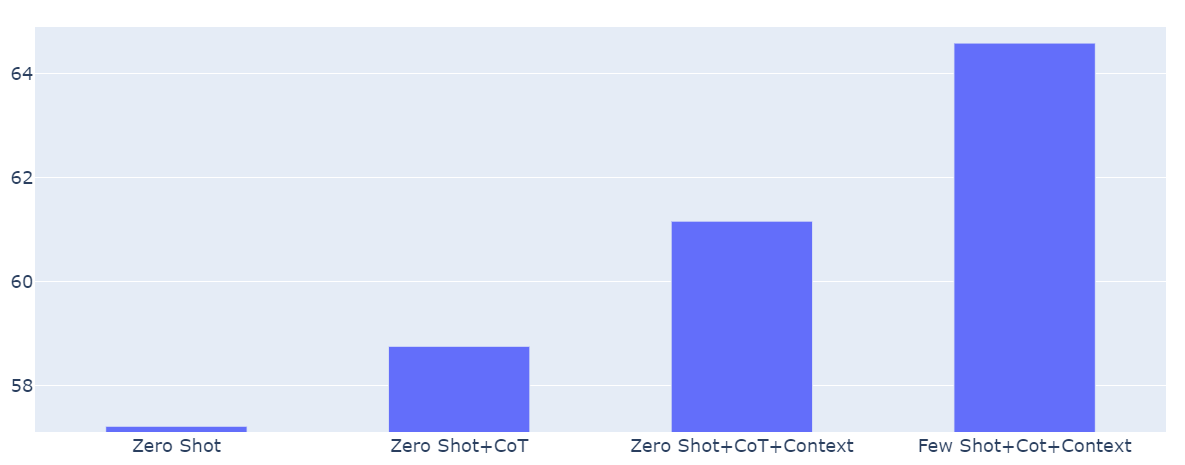
\includegraphics[width=0.9\linewidth]{images/prompt-result.png}}
	\caption{مقدار
		\lr{F1-Score}
		هر یک از تکنیک‌های پیش‌پردازش داده}
	\label{prompt-result-chart}
\end{figure}


 
در ادامه برای بررسی اثربخشی پیش‌پردازش متن ورودی بر خروجی مدل زبانی بزرگ، آزمایش‌ها برای پرامپت
\lr{Zero Shot + CoT + Context}
تکرار شد. در این آزمایش‌ها سه روش متفاوت برای پیش‌پردازش داده‌ها را که در فصل قبل عملکرد بهتری از خود نشان دادند مورد بررسی قرار گرفت. نتایج به دست آمده در جدول~
\ref{prompt-data-cleaning-impact}
گزارش شده است. در نمودار
\ref{prompt-data-cleaning-impact-chart}
نتایج به دست آمده به صورت شهودی قابل مقایسه است. همان‌طور که نتایج نشان می‌دهد، با تغییر روش پیش‌پردازش داده‌ها تغییر معنی‌داری در نتایج به دست آمده به وجود نمی‌آید. 
\begin{table}[h!]
	\centering
	\small
	\caption{\label{prompt-data-cleaning-impact}تاثیر پیش‌پردازش داده‌ها در نتایج به دست آمده}
	\vspace{0.2cm}
	\begin{tabular}{c  |c }
	\hline
	پیش‌پردازش & $F1-Score$\\
	\hline
	
	%Data prompt precirion Recall F1 accuract
	
	%Run8 Real Data P6 0.6233 0.6122 0.6116	0.6197	
	بدون پیش‌پردازش&  $61.16$
	%& $61.97$
	\\
	
	%Run12 Remove url P6 0.6268	0.6090	0.6157	0.6114
	حذف آدرس اینترنتی&  $61.57$\\
	%Run13 Remove username P6 0.6283 0.6216	0.6119	0.6236
حدف نام کاربری&  $61.19$\\
	%Run14	Remove url+username P6	0.6261	0.6102	0.6165	0.6069	
	حذف همزمان آدرس اینترنتی و نام کاربری&  $61.65$\\
	\hline
	\hline
\end{tabular}
\end{table}

\begin{figure}[H]
	\center{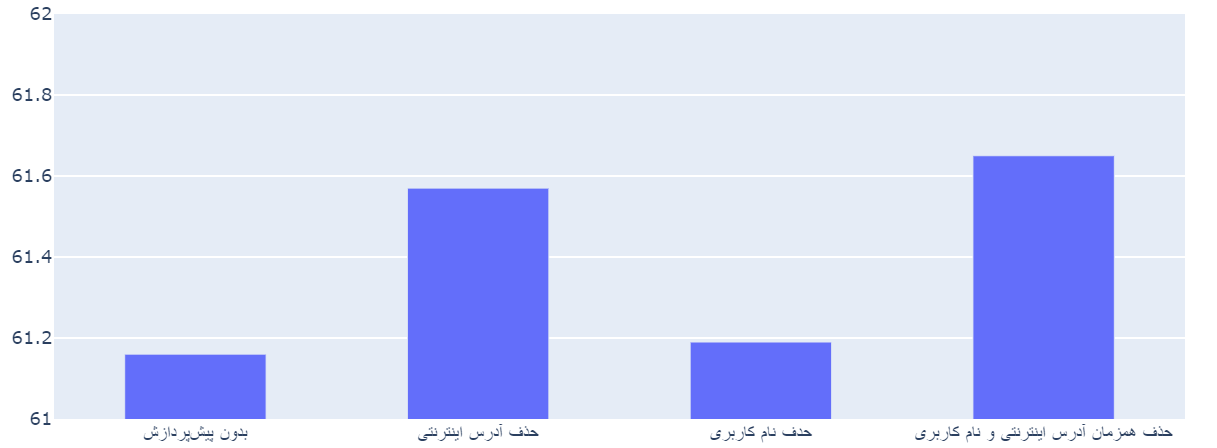
\includegraphics[width=0.9\linewidth]{images/prompt-data-cleaning-impact-chart.png}}
	\caption{مقدار
		\lr{F1-Score}
		هر یک از تکنیک‌های پیش‌پردازش داده}
	\label{prompt-data-cleaning-impact-chart}
\end{figure}


\subsection{مزایا و معایب روش پیشنهادی}
از جمله مزایای روش پیشنهادی، پیش‌بینی خروجی بدون نیاز به داده‌ آموزشی یا با وجود داده‌های آموزشی کم می‌باشد. بر خلاف روش فصل پنجم، استفاده از پرامپت 
\lr{Domain Specific}
نیست و بر دامنه‌های مختلف می‌توان نتایج قابل قبولی دریافت کرد.

از طرفی نیاز به منابع محاسباتی 
\lr{GPU}
با رم بالا از جمله معایب این روش می‌باشد. همچنین به دلیل اینکه پرامپت توسط نیروی انسانی طراحی می‌شود، ممکن است پرامپت کاملا بهینه‌ای طراحی نشده باشد. علاوه امکان 
\lr{fine-tuning}
پرامپت‌های پیشنهادی برای مدل با توجه به منابع محاسباتی محدود، مقدور نمی‌باشد.
\subsection{نحوه پیاده‌سازی و اجرا آزمایش‌ها}
پیاده‌سازی پروژه در 
\href{https://github.com/ghazaleh-mahmoodi/Climate_Activism_Stance_Detection}{اینجا}
\LTRfootnote{\href{https://github.com/ghazaleh-mahmoodi/Climate_Activism_Stance_Detection}{https://github.com/ghazaleh-mahmoodi/Climate\_Activism\_Stance\_Detection}}
قابل مشاهده می‌باشد که با زبان پایتون و فریم‌ورک پایتورچ انجام شده است. برای تعامل با مدل زبانی بزرگ از 
\lr{guidance}\LTRfootnote{\href{https://github.com/guidance-ai/guidance}{https://github.com/guidance-ai/guidance}}
استفاده شده است. هر بار پیشبینی برای کل داده‌های ارزیابی با توجه به نوع پرامپت حدود 40 الی 160 دقیقه زمان می‌برد. زمان تقریبی تولید خروجی برای یک ورودی حدود 4 الی 15 ثانیه می‌باشد.
\newline
برای اجرا از سخت‌افزار
\lr{GPU.1080Ti.xlarge}
با رم 
\lr{31.3GB}
استفاده شد. دستور 
\lr{nvidia-smi}
میزان استفاده از 
\lr{GPU}
را نمایش می‌دهد. خروجی این دستور در هنگام اجرا آزمایشات به صورت شکل 
\ref{nvidia-smi-prompt} شد.
\begin{figure}[H]		  		    			  	 \center{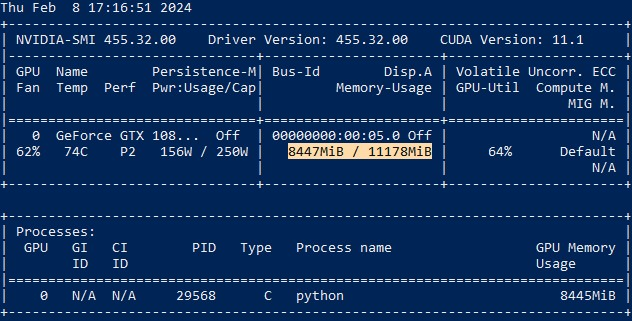
\includegraphics[width=0.8\linewidth]{images/nvidia-smi-prompt.jpg}}
	\caption{میزان مصرف \lr{GPU}در زمان اجرا آزمایش‌های مدل‌های زبانی بزرگ}
	\label{nvidia-smi-prompt}
\end{figure}

%\section{جمع‌بندی}


 
% !TeX root=main.tex
\chapter{نتیجه‌گیری و کارهای آینده}
\thispagestyle{empty}

\section{نتیجه‌گیری}
در این پژوهش روش‌های حل مسئله تشخیص موضع مورد بررسی قرار گرفت. در فصل پنجم، با الهام‌گیری از رویکرد جستجو معماری عصبی، برای طراحی مدل تشخیص موضع یک فضا جستجو تعریف شد. سپس یک جستجو قاعده‌مند صورت گرفت. همچنین اثربخشی روش پیش‌پردازش داده، افزایش داده، رده‌بند و تابع ضرر به صورت جداگانه مورد بررسی قرار گرفت. در نهایت کدگذار
\lr{BERTweet}
و رده‌بند
\lr{CNN}
به عنوان مدل پیشنهادی معرفی شد. افرایش داده و روش پیش‌پردازش با رویکرد حذف نام کاربری توانستند نتایج مدل را به صورت معناداری بهبود بدهند. رده‌یند
\lr{CNN}
به صورت معنا داری از 
\lr{FNN}
بهتر عمل می‌کند. روش جستجو ارائه شده عملکرد خوبی در طراحی یک معماری مناسب از خود نشان داد. 

در فصل ششم، چهار پرامپت با رویکردهای متفاوت و سلسله مراتبی برای حل مسئله تشخیص موضع بدون داده‌ آموزشی معرفی شد. در مجموعه داده
\lr{ClimaConvo}
پرامپت
\lr{Few Shot + Chain of Thought + Context}
بهترین نتیجه را در مقایسه با سایر رویکردها کسب کرد. در مجموعه داده 
\lr{SemEval}
پرامپت
\lr{Zero Shot}
پیشنهادی توانست در موضوع "قانونی شدن سقط جنین (\lr{LA})" مقدار
$ 2.03 $
 درصد در مقایسه یا روش‌های دیگر
\lr{Zero Shot}
بهبود داشته باشد. آزمایش‌ها نشان دادند، نحوه پیش‌پردازش داده در عملکرد مدل زبانی بزرگ تاثیر معناداری ایجاد نمی‌کند. از آن‌جا که جمع‌آوری داده به ازای همه موضوعات به راحتی میسر نمی‌باشد، با ادامه پژوهش در این زمینه (تشخیص موضع بدون داده‌ آموزشی) می‌توان گامی در جهت استفاده از تشخیص موضع در کابردهای زندگی روزمره برداشت.
 
\section{پیشنهادها و کار‌های آینده}

برای ادامه پژوهش در مسئله تشخیص موضع با نظارت موارد زیر پیشنهاد می‌شود.
\begin{enumerate}
	\item 
در این پژوهش تنها مدل‌های کدگذار (همچون
\lr{BRET})
مورد بررسی قرار گرفتند. در ادامه پیشنهاد می‌شود عملکرد مدل‌های کدگشا همانند
\lr{GPT-2}
و کدگذار-کدگشا همچون
\lr{BART, T5}
نیز مورد مقایسه قرار بگیرد.

\item
مدل‌های مبتنی بر درخت همچون
\lr{XGBoost}
اخیرا به نتایج خوبی در مسائل رده‌بندی دست یافتند. پیشنهاد می‌شود در ادامه تحقیقات عملکرد این مدل نیز مورد بررسی قرار بگیرد. از جمله مزایای مدل‌های مبتنی بر درخت تقسیرپذیر بودن می‌باشد.

\item
برای داده‌های نامتوازن از تابع‌ ضررهای متناسب استفاده می‌شود. در این پژوهش دو تابع ضرر معروف این حوزه مورد بررسی قرار گرفت. بررسی سایر تابع‌های ضرر از جمله
\lr{dice}
پیشنهاد می‌شود. همچنین ترکیب تابع ضررهای متفاوت می‌تواند نتایج خوبی به ارمغان بیاورد.

\item در بخش کدگذار می‌توان از چندین مدل از پیش‌آموزش دیده و 
\lr{Concat}
بازنمایی کلمات مربوط به آن‌ها استفاده کرد. 

\end{enumerate}


در رویکرد بدون داده‌ آموزشی برای ادامه تحقیقات پیشنهادات زیر ارائه می‌شود.
\begin{enumerate}
	\item
	در پژوهش فعلی در پرامپت
	\lr{Few Shot} 
	نمونه‌های آموزشی به صورت تصادفی انتخاب شدند. پیشنهاد می‌شود با استفاده بازنمایی کلمات، به جای انتخاب تصادفی نمونه‌های ورودی نمونه‌هایی که بیشترین مشابهت را با ورودی فعلی دارند به عنوان نمونه آموزشی انتخاب شوند. 
		\item
		با استفاده از روش‌های 
		\lr{Prefix-Tuning}
		می‌توان با ثابت نگه‌داشتن وزن‌های مدل و تنها آموزش 1 درصد وزن‌ها، نتایج بهتری با پرامپت تولیدی به دست آورد.
		
		
		\item تغییر پرامپت به صورتی که به ازای پیشبینی کلاس نهایی به صورت مستقیم، احتمال تعلق ورودی به هر کلاس را پیشبینی کند. در ادامه با ایده‌های سلسه مراتبی دیگر می‌توان کلاس نهایی را به دست آورد. به عنوان مثال می‌توان بین خروجی چند مدل زبانی بزرگ اجتماع گرفت.

\end{enumerate}





\pagestyle{empty}
{
\onehalfspacing
\bibliographystyle{acm-fa}%{plainnat-fa}%{chicago-fa}%{acm-fa}
\bibliography{Ref}
}

\pagestyle{fancy}

\onehalfspacing
\chapter*{واژه‌نامه فارسی به انگلیسی}\markboth{واژه‌نامه فارسی به انگلیسی}{واژه‌نامه فارسی به انگلیسی}
\addcontentsline{toc}{chapter}{واژه‌نامه فارسی به انگلیسی}
\thispagestyle{empty}

\englishgloss{Pre-tranin}{آموزش اولیه}
\englishgloss{Train}{آموزشی}
\englishgloss{Hyperparameter}{ابرپارامتر}
\englishgloss{Adaptive Selection}{انتخاب تطبیقی}
\englishgloss{Embedding}{بازنمایی کلمات}
\englishgloss{Paraphrase}{بازنویسی}
\englishgloss{Information Retrieval}{بازیابی اطلاعات}
\englishgloss{None/Neither/Neutral}{بدون نظر}
\englishgloss{Context vector}{بردار زمینه}
\englishgloss{Query vector}{بردار پرس‌وجو}
\englishgloss{Optimizer}{بهینه‌ساز}
\englishgloss{Prompt}{پرامپت}
\englishgloss{Attention}{توجه}
\englishgloss{Token}{توکن}
\englishgloss{Loss Function}{تابع ضرر}
\englishgloss{Humor Detection}{تشخیص طنز}
\englishgloss{Stance Detection}{تشخیص موضع}
\englishgloss{Hate Speach Detection}{تشخیص سخنان نفرت انگیز}
\englishgloss{Aspect-Oriented Sentiment Analysis}{تحلیل احساسات جنبه گرا}
\englishgloss{Self-attention}{توجه به خود}
\englishgloss{Early Stopping}{توقف زود هنگام}
\englishgloss{Grid Search}{جستجو شبکه‌ای}
\englishgloss{URL}{حذف آدرس‌ اینترنتی}
\englishgloss{Imbalance data}{داده‌های نامتوازن}
\englishgloss{Temperature}{دما}
\englishgloss{Epoch}{دوره}
\englishgloss{Classifier}{رده‌بند}
\englishgloss{Social Media}{شبکه‌های اجتماعی}
\englishgloss{Recurrent Neural Network (RNN)}{شبکه‌ عصبی بازگشتی}
\englishgloss{Fully Connected Neural Networks}{شبکه عصبی تماما متصل}
\englishgloss{Convolutional neural network}{شبکه عصبی پیچشی}
\englishgloss{Systematic}{قاعده‌مند}
\englishgloss{Legalization of Abortion}{قانونی شدن سقط جنین}
\englishgloss{encoder}{کدگذار}
\englishgloss{Decoder}{کدگشا‍}
\englishgloss{Encoder-Decoder}{کدگذار-کدگشا}
\englishgloss{Stop Words}{کلمه‌های توقف}
\englishgloss{Lower Casing}{کوچک کردن حروف}
\englishgloss{Classification Task}{مسائل رده‌بندی}
\englishgloss{Development Set}{مجموعه توسعه}
\englishgloss{Vanishing Gradient}{محو شدگی گرادیان}
\englishgloss{Against/Oppose}{مخالف}
\englishgloss{Large Language Models (LLMs)}{مدل‌های زبانی بزرگ}
\englishgloss{Significance}{معنادار}
\englishgloss{Support/Favor}{موافق}
\englishgloss{Prompt Engineering}{مهندسب پرامپت}
\englishgloss{Stance}{موضع‌گیری}
\englishgloss{Macro Average}{میانگین کلان}
\englishgloss{Username}{نام‌کاربری}
\englishgloss{Curse of Dimensionality}{نفرین ابعاد}
\englishgloss{Climate Change is Concern}{نگرانی از تغییرات آب و هوایی}
\englishgloss{Feature}{ویژگی}
\englishgloss{Target}{هدف}
\englishgloss{ّIn-context learning}{یادگیری درون متنی}
\englishgloss{Adversarial Learning}{یادگیری تقابلی}

\chapter*{واژه‌نامه  انگلیسی به  فارسی}\markboth{واژه‌نامه  انگلیسی به  فارسی}{واژه‌نامه  انگلیسی به  فارسی}
\addcontentsline{toc}{chapter}{واژه‌نامه  انگلیسی به  فارسی}
\thispagestyle{empty}

\englishgloss{Adaptive Selection}{انتخاب تطبیقی}
\englishgloss{Adversarial Learning}{یادگیری تقابلی}
\englishgloss{Against}{مخالف}
\englishgloss{Aspect-Oriented Sentiment Analysis}{تحلیل احساسات جنبه گرا}
\englishgloss{Attention}{توجه}
\englishgloss{Classification Task}{مسائل رده‌بندی}
\englishgloss{Classifier}{رده‌بند}
\englishgloss{Climate Change is Concern}{نگرانی از تغییرات آب و هوایی}
\englishgloss{Context vector}{بردار زمینه}
\englishgloss{Convolutional neural network}{شبکه عصبی پیچشی}
\englishgloss{Curse of Dimensionality}{نفرین ابعاد}
\englishgloss{Decoder}{کدگشا‍}
\englishgloss{Development Set}{مجموعه توسعه}
\englishgloss{Early Stopping}{توقف زود هنگام}
\englishgloss{Embedding}{بازنمایی کلمات}
\englishgloss{Encoder}{کدگذار}
\englishgloss{Encoder-Decoder}{کدگذار-کدگشا}
\englishgloss{Epoch}{دوره}
\englishgloss{Favor}{موافق}
\englishgloss{Feature}{ویژگی}
\englishgloss{Fully Connected Neural Networks}{شبکه عصبی تماما متصل}
\englishgloss{Grid Search}{جستجو شبکه‌ای}
\englishgloss{Hate Speach Detection}{تشخیص سخنان نفرت انگیز}
\englishgloss{Humor Detection}{تشخیص طنز}
\englishgloss{Hyperparameter}{ابرپارامتر}
\englishgloss{Imbalance data}{داده‌های نامتوازن}
\englishgloss{ّIn-context learning}{یادگیری درون متنی}
\englishgloss{Information Retrieval}{بازیابی اطلاعات}
\englishgloss{Large Language Models (LLMs)}{مدل‌های زبانی بزرگ}
\englishgloss{Legalization of Abortion}{قانونی شدن سقط جنین}
\englishgloss{Loss Function}{تابع ضرر}
\englishgloss{Lower Casing}{کوچک کردن حروف}
\englishgloss{Macro Average}{میانگین کلان}
\englishgloss{None/Neither/Neutral}{بدون نظر}
\englishgloss{Optimizer}{بهینه‌ساز}
\englishgloss{Oppose}{مخالف}
\englishgloss{Paraphrase}{بازنویسی}
\englishgloss{Pre-tranin}{آموزش اولیه}
\englishgloss{Prompt}{پرامپت}
\englishgloss{Prompt Engineering}{مهندسب پرامپت}
\englishgloss{Query vector}{بردار پرس‌وجو}
\englishgloss{Recurrent Neural Network (RNN)}{شبکه‌ عصبی بازگشتی}
\englishgloss{Self-attention}{توجه به خود}
\englishgloss{Significance}{معنادار}
\englishgloss{Social Media}{شبکه‌های اجتماعی}
\englishgloss{Stance}{موضع‌گیری}
\englishgloss{Stance Detection}{تشخیص موضع}
\englishgloss{Stop Words}{کلمه‌های توقف}
\englishgloss{Support}{موافق}
\englishgloss{Systematic}{قاعده‌مند}
\englishgloss{Target}{هدف}
\englishgloss{Temperature}{دما}
\englishgloss{Train}{آموزشی}
\englishgloss{Token}{توکن}
\englishgloss{URL}{حذف آدرس‌ اینترنتی}
\englishgloss{Username}{نام‌کاربری}
\englishgloss{Vanishing Gradient}{محو شدگی گرادیان}

\printindex

% !TeX root=main.tex
% در این فایل، عنوان پایان‌نامه، مشخصات خود و چکیده پایان‌نامه را به انگلیسی، وارد کنید.

%%%%%%%%%%%%%%%%%%%%%%%%%%%%%%%%%%%%
\baselineskip=.6cm
\begin{latin}
\latinuniversity{Iran University of Science and Technology}
\latinfaculty{Computer Engineering Department}
\latinsubject{Computer Engineering }
\latinfield{Artificial Intelligence}
\latintitle{Stance Detection for Textual Content in Social Media}
\firstlatinsupervisor{Dr. Sayyed Sauleh Eetemadi}

\latinname{Ghazaleh}
\latinsurname{Mahmoudi}
\latinthesisdate{February  2024}
\latinkeywords{Stance Detection for Textual Content in Social Media}
\en-abstract{
Nowadays, social media is a platform for freely expressing and sharing opinions and thoughts. This leads to the fact that by analyzing the data available on social media, a broad and comprehensive perspective on various users’ opinions and sides about different topics could be gained. These topics include political, economic, social, and cultural issues. In Natural Language Processing, stance detection is the process of automatically recognizing the side and stance of a given text about a
specific target. 
\newline
In natural language processing tasks, the way text data is preprocessed significantly affects the performance of the trained model. In this research, seven different levels of preprocessing are introduced and examined. Additionally, to find the architecture of the stance detection model, the idea of Neural Architecture Search (NAS) was inspired. In this method, the model architecture is divided into four main parts, a search space is defined for each part, and adaptive search algorithms are used to design the final architecture. The best proposed model ultimately utilizes BERTweet as the encoder and a CNN classifier. The proposed architecture achieved an F1-Score of 74.47\%, showing a 19.97\% improvement over the Baseline model. Furthermore, the proposed method ranked third among 19 participants in a climate change stance detection event. Additionally, due to the lack of training data for different topics, stance detection without training data was also investigated. This approach, which uses large language models and prompt engineering, introduces four approaches based on different prompt types. Then, the performance of the proposed prompts was compared with other methods for stance detection without training data. The introduced approach achieved an F1-Score of 57.33\%, showing a 2.03\% improvement over similar approaches.}
\latinfirstPage
\end{latin}

\label{LastPage}

\end{document}